
\documentclass[12pt,reqno]{amsart}
%%%%%%%%%%%%%%%%%%%%%%%%%%%%%%%%%%%%%%%%%%%%%%%%%%%%%%%%%%%%%%%%%%%%%%%%%%%%%%%%%%%%%%%%%%%%%%%%%%%%%%%%%%%%%%%%%%%%%%%%%%%%%%%%%%%%%%%%%%%%%%%%%%%%%%%%%%%%%%%%%%%%%%%%%%%%%%%%%%%%%%%%%%%%%%%%%%%%%%%%%%%%%%%%%%%%%%%%%%%%%%%%%%%%%%%%%%%%%%%%%%%%%%%%%%%%
\usepackage{mathtools}
\usepackage{amsfonts}
\usepackage[utf8]{inputenc}
\usepackage{amsmath,amssymb,amsthm}
\usepackage{float}
\usepackage{array}
\usepackage{graphicx}
\usepackage{setspace}
\usepackage{xcolor}
\usepackage{enumitem}
\usepackage[margin=17mm]{geometry}
\usepackage{tikz}
\usepackage{fancyvrb}
\usepackage{fancyhdr}
\usepackage{titlesec,titletoc}
\usepackage[colorlinks=true,linkcolor=blue,citecolor=green,urlcolor=magenta]{hyperref}
\usepackage{aliascnt}
\usepackage[nameinlink]{cleveref}
\usepackage{listings}
\usepackage{booktabs}

\setcounter{MaxMatrixCols}{10}
%TCIDATA{OutputFilter=LATEX.DLL}
%TCIDATA{Version=5.50.0.2960}
%TCIDATA{<META NAME="SaveForMode" CONTENT="1">}
%TCIDATA{BibliographyScheme=Manual}
%TCIDATA{LastRevised=Tuesday, November 24, 2026 17:46:43}
%TCIDATA{<META NAME="GraphicsSave" CONTENT="32">}

\setlength{\tabcolsep}{3pt}
\renewcommand{\arraystretch}{1.35}
\renewcommand{\tablename}{$\textsf{Tab}$}
\setlength{\tabcolsep}{3pt}
\renewcommand{\arraystretch}{1.2}
\newcommand{\N}{\mathbb N}
\newcommand{\Z}{\mathbb Z}
\newcommand{\Q}{\mathbb Q}
\newcommand{\R}{\mathbb R}
\newcommand{\C}{\mathbb C}
\newcommand{\Np}{\N_{\ge1}}
\newcommand{\fl}[1]{\left\lfloor #1\right\rfloor}
\providecommand{\TEXTsymbol}[1]{#1}
\makeatletter
\newcommand{\SplitTableCaption}{\def\@captype{table}\caption}
\makeatother
\restylefloat{figure}
\hypersetup{pageanchor=false}
\makeatletter
\@ifundefined{theorem}{}{\let\theorem\relax}
\@ifundefined{definition}{}{\let\definition\relax}
\@ifundefined{lemma}{}{\let\lemma\relax}
\@ifundefined{corollary}{}{\let\corollary\relax}
\@ifundefined{proposition}{}{\let\proposition\relax}
\@ifundefined{remark}{}{\let\remark\relax}
\@ifundefined{statement}{}{\let\statement\relax}
\makeatother
\DeclareUnicodeCharacter{03B9}{\ensuremath{\iota}}
\DeclareUnicodeCharacter{2200}{\ensuremath{\forall}}
\DeclareUnicodeCharacter{2203}{\ensuremath{\exists }}
\DeclareUnicodeCharacter{2208}{\ensuremath{\in}}
\DeclareUnicodeCharacter{2218}{\ensuremath{\circ}}
\DeclareUnicodeCharacter{2264}{\ensuremath{\leq}}
\DeclareUnicodeCharacter{2265}{\ensuremath{\geq}}
\DeclareUnicodeCharacter{2192}{\ensuremath{\to}}
\DeclareUnicodeCharacter{21A6}{\ensuremath{\mapsto}}
\DeclareUnicodeCharacter{2260}{\ensuremath{\neq}}
\DeclareUnicodeCharacter{00D7}{\ensuremath{\times}}
\DeclareUnicodeCharacter{2115}{\ensuremath{\mathbb{N}}}
\DeclareUnicodeCharacter{211D}{\ensuremath{\mathbb{R}}}
\DeclareUnicodeCharacter{27E8}{\ensuremath{\langle}}
\DeclareUnicodeCharacter{27E9}{\ensuremath{\rangle}}
\providecommand{\period}{\,\allowbreak}
\newcommand{\pagenumside}{C}
\newlength{\pageNumberOffset}
\setlength{\pageNumberOffset}{0pt}
\newcommand{\PagenumSideC}{C}
\newcommand{\applypagehead}[1]{\expandafter\fancyhead\expandafter[\pagenumside]{#1}\ifx\pagenumside\PagenumSideC\else\ifdim\pageNumberOffset=0pt\else\expandafter\fancyheadoffset\expandafter[\pagenumside]{\pageNumberOffset}\fi\fi}
\newcommand{\applypagefoot}[1]{\expandafter\fancyfoot\expandafter[\pagenumside]{#1}\ifx\pagenumside\PagenumSideC\else\ifdim\pageNumberOffset=0pt\else\expandafter\fancyfootoffset\expandafter[\pagenumside]{\pageNumberOffset}\fi\fi}
\pagestyle{fancy}
\fancyhf{}
\applypagehead{\thepage}
\renewcommand{\headrulewidth}{0pt}
\renewcommand{\footrulewidth}{0pt}
\fancypagestyle{plain}{\fancyhf{}\applypagehead{\thepage}\renewcommand{\headrulewidth}{0pt}}
\setlength{\arraycolsep}{1.5pt}
\setlength{\tabcolsep}{1.5pt}
\renewcommand{\arraystretch}{1.0}
\setlength{\arrayrulewidth}{0.4pt}
\setlength{\doublerulesep}{1pt}
\setlength{\extrarowheight}{0pt}
\newcolumntype{C}{>{\centering\arraybackslash\scriptsize}m{40pt}}
\newcolumntype{R}{>{\centering\arraybackslash\scriptsize}m{2.5cm}}
\newcolumntype{L}{>{\centering\arraybackslash\scriptsize}m{10.5cm}}
\fvset{frame=lines,framerule=0.7pt,rulecolor=\color{blue!60!black},framesep=2pt,fontsize=\scriptsize,xleftmargin=4pt,xrightmargin=4pt}
\RecustomVerbatimEnvironment{verbatim}{Verbatim}{}
\DefineVerbatimEnvironment{verbatimbox}{Verbatim}{frame=single,framerule=0.7pt,rulecolor=\color{blue!60!black},framesep=2pt,fontsize=\scriptsize,xleftmargin=4pt,xrightmargin=4pt}
\makeatletter
\def\@setsubjclass{\ifx\@subjclass\@empty\else\@subjclass\fi}
\makeatother
\subjclass{\textbf{2020 Mathematics Subject Classification.}\,Primary 28A12.}
\keywords{dominated convergence, monotone convergence, nonnegative integration, almost-everywhere convergence, typed proofs}
\renewcommand{\abstractname}{\fontsize{9}{11}\selectfont Abstract}
\newcommand{\abstractfont}{\normalfont\fontsize{8}{10}\selectfont}
\newcommand{\abstractheadingsep}{\vspace{0.5em}}
\makeatletter
\renewenvironment{abstract}{\ifx\maketitle\relax\ClassWarning{\@classname}{Abstract should precede\protect\maketitle\space in AMS document classes reported}\fi\global\setbox\abstractbox=\vtop \bgroup\abstractfont{\centering\abstractname\par}\abstractheadingsep\list{}{\labelwidth\z@\leftmargin3pc \rightmargin\leftmargin\listparindent\normalparindent \itemindent\z@\parsep\z@ \@plus\p@\let\fullwidthdisplay\relax}\item\relax}{\endlist\egroup\ifx\@setabstract\relax \@setabstracta \fi}
\makeatother
\setcounter{secnumdepth}{3}
\newcommand{\SecAbove}{1.0ex plus 0.3ex minus 0.1ex}
\newcommand{\SecBelow}{0pt}
\newcommand{\SubsecAbove}{0.8ex plus 0.2ex minus 0.1ex}
\newcommand{\SubsecBelow}{0pt}
\newcommand{\SubsubsecAbove}{0.6ex plus 0.2ex minus 0.1ex}
\newcommand{\SubsubsecBelow}{0pt}
\makeatletter
\titleformat{\section}{\normalfont\fontsize{16}{18}\selectfont\bfseries}{\thesection.}{0.5em}{}
\titleformat{\subsection}{\normalfont\fontsize{14}{16}\selectfont\bfseries}{\thesubsection.}{0.5em}{}
\titleformat{\subsubsection}{\normalfont\fontsize{12}{14}\selectfont\bfseries}{\thesubsubsection.}{0.5em}{}
\titlespacing*{\section}{\z@}{\SecAbove}{\SecBelow}
\titlespacing*{\subsection}{\z@}{\SubsecAbove}{\SubsecBelow}
\titlespacing*{\subsubsection}{\z@}{\SubsubsecAbove}{\SubsubsecBelow}
\makeatother
\newcounter{axctr}\newcounter{posctr}
\newcounter{lemctr}\newcounter{thmctr}\newcounter{asserctr}\newcounter{corctr}
\renewcommand{\theaxctr}{\arabic{axctr}}
\renewcommand{\theposctr}{\arabic{posctr}}
\renewcommand{\thelemctr}{\arabic{lemctr}}
\renewcommand{\thethmctr}{\arabic{thmctr}}
\renewcommand{\theasserctr}{\arabic{asserctr}}
\renewcommand{\thecorctr}{\arabic{corctr}}
\renewcommand{\theHaxctr}{\thesection.\arabic{axctr}}
\renewcommand{\theHposctr}{\thesection.\arabic{posctr}}
\renewcommand{\theHlemctr}{\thesection.\arabic{lemctr}}
\renewcommand{\theHthmctr}{\thesection.\arabic{thmctr}}
\renewcommand{\theHasserctr}{\thesection.\arabic{asserctr}}
\providecommand{\theHasser}{\theequation}
\renewcommand{\theHcorctr}{\thesection.\arabic{corctr}}
\newcommand{\swpax}[2]{\refstepcounter{axctr}\hypertarget{#1}{\mbox{\textbf{Ax\,\theaxctr}}}\label{#2}}
\newcommand{\swppos}[2]{\refstepcounter{posctr}\hypertarget{#1}{\mbox{\textbf{Pos\,\theposctr}}}\label{#2}}
\newcommand{\swplem}[2]{\refstepcounter{lemctr}\hyperlink{#1}{\mbox{\textbf{Lem\,\thelemctr}}}\label{#2}}
\newcommand{\swpthm}[2]{\refstepcounter{thmctr}\hyperlink{#1}{\mbox{\textbf{Thm\,\thethmctr}}}\label{#2}}
\newcommand{\swpcor}[2]{\refstepcounter{corctr}\hypertarget{#1}{\mbox{\textbf{Cor\,\thecorctr}}}\label{#2}}
\newcommand{\tagged}[2]{\hypertarget{#1}{\mbox{\textbf{#2}}}}
\newcommand{\autorefto}[2]{\hyperlink{#1}{#2}}
\newcommand{\mcite}[1]{\text{\cite{#1}}}
\newtheoremstyle{blueplain}{2pt plus 1pt minus 0.5pt}{1pt plus 0.5pt minus 0.3pt}{\itshape}{}{\bfseries\color{blue}}{.}{\newline}{\thmname{#1}\thmnumber{ #2}\thmnote{ {\bfseries\color{blue}(#3)}}}
\theoremstyle{blueplain}
\newtheorem{theorem}{Theorem}[section]
\newtheorem{lemma}{Lemma}[section]
\newtheorem{corollary}{Corollary}[section]
\newtheorem{proposition}{Proposition}[section]
\newtheorem{remark}{Remark}[section]
\newtheorem*{definition}{Definition}
\newtheorem{statement}{Statement}[section]
\definecolor{proofhead}{RGB}{11,83,148}
\definecolor{proofqed}{RGB}{204,0,0}
\renewcommand{\qedsymbol}{\textcolor{proofqed}{\ensuremath{\square}}}
\renewenvironment{proof}[1][Proof]{\par\noindent\textbf{\textcolor{proofhead}{#1.}}\par\nobreak}{\par\nobreak\hfill\qedsymbol}
\newenvironment{swpproof}[1][Proof]{\begin{proof}[#1]}{\end{proof}}
\renewcommand{\theHtheorem}{\thesection.\arabic{theorem}}
\renewcommand{\theHstatement}{\thesection.\arabic{statement}}
\providecommand{\axctrautorefname}{Axiom}
\providecommand{\posctrautorefname}{Postulate}
\providecommand{\lemctrautorefname}{Lemma}
\providecommand{\thmctrautorefname}{Theorem}
\providecommand{\asserctrautorefname}{Proposition}
\providecommand{\corctrautorefname}{Corollary}
\providecommand{\statementautorefname}{Statement}
\crefname{axctr}{axiom}{axioms}
\crefname{posctr}{postulate}{postulates}
\crefname{lemctr}{lemma}{lemmas}
\crefname{thmctr}{theorem}{theorems}
\crefname{asserctr}{proposition}{propositions}
\crefname{corctr}{corollary}{corollaries}
\Crefname{axctr}{Axiom}{Axioms}
\Crefname{posctr}{Postulate}{Postulates}
\Crefname{lemctr}{Lemma}{Lemmas}
\Crefname{thmctr}{Theorem}{Theorems}
\Crefname{asserctr}{Proposition}{Propositions}
\Crefname{corctr}{Corollary}{Corollaries}
\crefname{statement}{statement}{statements}
\Crefname{statement}{Statement}{Statements}
\crefname{section}{section}{sections}
\Crefname{section}{Section}{Sections}
\crefname{equation}{eq}{eqs}
\Crefname{equation}{Eq}{Eqs}
\crefformat{equation}{#2\textcolor{blue}{eq~#1}#3}
\Crefformat{equation}{#2\textcolor{blue}{Eq~#1}#3}
\newcounter{inq}
\renewcommand{\theinq}{\theequation}
\makeatletter
\renewcommand{\p@inq}{\p@equation}
\makeatother
\crefname{inq}{ineq}{inequalities}
\Crefname{inq}{Ineq}{Inequalities}
\crefformat{inq}{#2\textcolor{blue}{inequality~#1}#3}
\Crefformat{inq}{#2\textcolor{blue}{Inequality~#1}#3}
\crefmultiformat{inq}{#2\textcolor{blue}{inequalities~#1}#3}{\textcolor{blue}{ ,\,~#2#1#3}}{\textcolor{blue}{, #2#1#3}}{\textcolor{blue}{ ,\,~#2#1#3}}
\Crefmultiformat{inq}{#2\textcolor{blue}{Inequalities~#1}#3}{\textcolor{blue}{ ,\,~#2#1#3}}{\textcolor{blue}{, #2#1#3}}{\textcolor{blue}{ ,\,~#2#1#3}}
\makeatletter
\newenvironment{ineq}
{\begin{equation}\refstepcounter{inq}}
{\end{equation}}
\makeatother
\newcounter{type}
\renewcommand{\thetype}{\theequation}
\makeatletter
\renewcommand{\p@type}{\p@equation}
\makeatother
\crefname{type}{type}{types}
\Crefname{type}{Type}{Types}
\crefformat{type}{#2\textcolor{blue}{type~#1}#3}
\Crefformat{type}{#2\textcolor{blue}{Type~#1}#3}
\crefmultiformat{type}{#2\textcolor{blue}{types~#1}#3}{\textcolor{blue}{ ,\,~#2#1#3}}{\textcolor{blue}{, #2#1#3}}{\textcolor{blue}{ ,\,~#2#1#3}}
\Crefmultiformat{type}{#2\textcolor{blue}{Types~#1}#3}{\textcolor{blue}{ ,\,~#2#1#3}}{\textcolor{blue}{, #2#1#3}}{\textcolor{blue}{ ,\,~#2#1#3}}
\makeatletter
\newenvironment{type}
{\begin{equation}\refstepcounter{type}}
{\end{equation}}
\makeatother
\newcounter{asser}
\renewcommand{\theasser}{\theequation}
\makeatletter
\renewcommand{\p@asser}{\p@equation}
\makeatother
\crefname{asser}{Assertion}{assertions}
\Crefname{asser}{Assertion}{Assertions}
\crefformat{asser}{#2\textcolor{blue}{assertion~#1}#3}
\Crefformat{asser}{#2\textcolor{blue}{Assertion~#1}#3}
\crefmultiformat{asser}{#2\textcolor{blue}{assertions~#1}#3}{\textcolor{blue}{ ,\,~#2#1#3}}{\textcolor{blue}{, #2#1#3}}{\textcolor{blue}{ ,\,~#2#1#3}}
\Crefmultiformat{asser}{#2\textcolor{blue}{Assertions~#1}#3}{\textcolor{blue}{ ,\,~#2#1#3}}{\textcolor{blue}{, #2#1#3}}{\textcolor{blue}{ ,\,~#2#1#3}}
\makeatletter
\newenvironment{asser}
{\begin{equation}\refstepcounter{asser}}
{\end{equation}}
\makeatother
\newcommand{\thmref}[1]{\hyperref[#1]{Theorem~\ref*{#1}}}
\newcommand{\lemref}[1]{\hyperref[#1]{Lemma~\ref*{#1}}}
\newcommand{\corref}[1]{\hyperref[#1]{Corollary~\ref*{#1}}}
\newcommand{\propref}[1]{\hyperref[#1]{Proposition~\ref*{#1}}}
\makeatletter
\let\orig@maketitle\maketitle
\renewcommand{\maketitle}{\begingroup\let\MakeUppercase\@firstofone\let\uppercase\@firstofone\orig@maketitle\endgroup}
\newlength{\titleToAuthorSkip}
\newlength{\authorToAbstractSkip}
\setlength{\titleToAuthorSkip}{3pt plus 1pt minus 0.5pt}
\setlength{\authorToAbstractSkip}{4pt plus 1pt minus 0.5pt}
\renewcommand{\@maketitle}{\normalfont\normalsize\let\@makefnmark\relax\let\@thefnmark\relax\ifx\@empty\@subjclass\else\@footnotetext{\@setsubjclass}\fi\ifx\@empty\@keywords\else\@footnotetext{\@setkeywords}\fi\ifx\@empty\@thanks\else\@footnotetext{\@setthanks}\fi\@settitle\ifx\@empty\@authors\else\vspace{\titleToAuthorSkip}\@setauthors\fi\ifx\@empty\@date\else\vspace{3pt}\@setdate\fi\ifx\@empty\@abstract\else\vspace{\authorToAbstractSkip}\fi\@setabstract}
\makeatother
\makeatletter
\renewcommand{\encodingdefault}{OT1}
\makeatother
\renewcommand{\rmdefault}{cmr}
\renewcommand{\sfdefault}{cmss}
\renewcommand{\ttdefault}{cmtt}
\fontencoding{OT1}\fontfamily{cmr}\selectfont
\renewcommand{\contentsname}{\texorpdfstring{{\color{blue!60!black}\sffamily\Large\selectfont\bfseries Contents}}{Contents}}
\renewcommand{\seriesdefault}{\bfdefault}
\boldmath
\providecommand{\comma}{\allowbreak,\,}
\IfFileExists{tcilatex.tex}{\input{tcilatex}}{}
\makeatletter
\def\dudley@listtighten{  \setlength{\topsep}{0pt}  \setlength{\partopsep}{0pt}  \setlength{\itemsep}{1pt plus 0.5pt minus 0.3pt}  \setlength{\parsep}{0pt}  \setlength{\labelsep}{0.4em}}
\def\dudley@itemlabel{  \ifnum\@listdepth=\@ne \labelitemi
	\else\ifnum\@listdepth=\tw@ \labelitemii
	\else\ifnum\@listdepth=\thr@@ \labelitemiii
	\else \labelitemiv\fi\fi\fi}
\def\dudley@enumlabel{  \ifnum\@listdepth=\@ne \arabic{enumi}.
	\else\ifnum\@listdepth=\tw@ \alph{enumii}.
	\else\ifnum\@listdepth=\thr@@ \roman{enumiii}.
	\else \Alph{enumiv}.\fi\fi\fi}
\def\dudley@enumcounter{  \ifnum\@listdepth=\@ne \usecounter{enumi}  \else\ifnum\@listdepth=\tw@ \usecounter{enumii}  \else\ifnum\@listdepth=\thr@@ \usecounter{enumiii}  \else \usecounter{enumiv}\fi\fi\fi}
\makeatother
\setlength{\parindent}{0pt}
\setlength{\parskip}{0.25em plus 0.05em minus 0.05em}
\makeatletter
\renewenvironment{quotation}
{\list{}{\listparindent\z@
		\itemindent\z@
		\rightmargin\leftmargin
		\parsep\z@}	\item\relax}
{\endlist}
\makeatother
\numberwithin{equation}{section}
\newcolumntype{P}[1]{>{\centering\arraybackslash\scriptsize}m{#1}|}
\lstdefinestyle{python}{
	language=Python,
	basicstyle=\ttfamily\scriptsize,
	keywordstyle=\color{blue},
	commentstyle=\color{gray},
	stringstyle=\color{orange},
	numbers=left,
	numberstyle=\tiny,
	breaklines=true,
	frame=single,
	showstringspaces=false,
	xleftmargin=4pt,
	xrightmargin=4pt
}
\lstdefinestyle{lean}{
	language=ML,
	literate={θ}{{$\theta$}}1 {ε}{{$\varepsilon$}}1 {ℝ}{{$\mathbb R$}}1 {ℕ}{{$\mathbb N$}}1 {ℚ}{{$\mathbb Q$}}1 {·}{{$\cdot$}}1
	{∀}{{$\forall$}}1 {∃}{{$\exists$}}1 {∧}{{$\wedge$}}1
	{→}{{$\to$}}1 {←}{{$\leftarrow$}}1 {≤}{{$\le$}}1
	{⌊}{{$\lfloor$}}1 {⌋}{{$\rfloor$}}1 {₊}{{$_+$}}1
	{⟨}{{$\langle$}}1 {⟩}{{$\rangle$}}1,
	basicstyle=\ttfamily\scriptsize,
	keywordstyle=\color{blue},
	commentstyle=\color{gray},
	stringstyle=\color{orange},
	numbers=left,
	numberstyle=\tiny,
	breaklines=true,
	frame=single,
	showstringspaces=false,
	xleftmargin=4pt,
	xrightmargin=4pt
}
\setcounter{tocdepth}{1}
\contentsmargin{1em}
\titlecontents{part}[0pt]{\addvspace{14pt}\large\bfseries}{\makebox[2.0em][l]{\thecontentslabel.}}{}{\titlerule*[0.6pc]{.}\contentspage}[\addvspace{4pt}]
\titlecontents{section}[2.0em]{\addvspace{10pt}\small\bfseries}{\makebox[2.0em][l]{\thecontentslabel.}}{\hspace*{-2.0em}}{\titlerule*[0.6pc]{.}\contentspage}[\addvspace{2pt}]
\titlecontents{subsection}[4.5em]{\addvspace{4pt}\footnotesize}{\makebox[2.5em][l]{\thecontentslabel.}}{\hspace*{-2.5em}}{\titlerule*[0.6pc]{.}\contentspage}[\addvspace{1pt}]
\setlist[itemize]{topsep=0pt,partopsep=0pt,itemsep=1pt plus 0.5pt minus 0.3pt,parsep=0pt,leftmargin=1.5em,labelsep=0.4em,label=\textbullet}
\setlist[enumerate]{topsep=0pt,partopsep=0pt,itemsep=1pt plus 0.5pt minus 0.3pt,parsep=0pt,leftmargin=1.8em,labelsep=0.4em}
\newcommand{\defitem}[2]{\hypertarget{def:#1}{#2}}
\newcommand{\proofitem}[2]{\hypertarget{proof:#1}{#2}}
\DeclareRobustCommand{\proofref}[2]{\hyperlink{proof:#1}{\ensuremath{#2}}}
\pdfstringdefDisableCommands{  \def\proofref#1#2{#2}  \def\hyperlink#1#2{#2}}
\newcommand{\DeclareProofBlock}[2]{  \expandafter\def\csname ProofBlockName@#1\endcsname{#2}}
\newcommand{\stepitem}[3]{\hypertarget{proofstep:#1:#2}{#3}}
\DeclareRobustCommand{\stepref}[2]{  \hyperlink{proofstep:#1:#2}{\ensuremath{\csname ProofBlockName@#1\endcsname(#2)}}}
\DeclareRobustCommand{\steprangeref}[3]{  \hyperlink{proofstep:#1:#2}{\ensuremath{\csname ProofBlockName@#1\endcsname(#2\text{--}#3)}}}
\newlength{\DCTOneColumnBody}
\AtBeginDocument{\setlength{\DCTOneColumnBody}{0.9\textwidth}\addtolength{\DCTOneColumnBody}{6\tabcolsep}\addtolength{\DCTOneColumnBody}{3\arrayrulewidth}}

\begin{document}
\title{{\Large Dominated Convergence Theorem in Lean}\\
[4pt] {\normalsize A Typed Mathematical Presentation}}
\author{%
\bfseries{\large \hspace{1.2in} Brahimi Mahdi Tahar\newline\text{ \
			} \newline\text{ \  } \hspace{0.5in}\text{ \  } University of Mohamed
			Boudiaf of M'sila, Algeria\newline\text{ \  }
			\newline\href{mailto:mahditahar.brahimi@univ-msila.dz}{mahditahar.brahimi@univ-msila.dz}}
}
\maketitle

{\centering {\small \setlength{\abovedisplayskip}{3pt}\setlength{%
\belowdisplayskip}{3pt}\ 
\begin{equation*}
\begin{gathered} f:\textsf{PosNat}\to X\to\textsf{Real},\quad
\ell:X\to\textsf{Real},\quad g:X\to\textsf{NNReal},\\[2pt]
\hyperlink{dctdef:DCTHyp}{\ensuremath{\textsf{DCTHyp}}}(f,\ell,g)
\Rightarrow(\forall n,\
\hyperlink{dctdef:Signed}{\ensuremath{\textsf{L1}}}(f_n))\land\textsf{L1}(%
\ell),\\[2pt] \textsf{DCTHyp}(f,\ell,g)\Rightarrow
\textsf{Conv}((\textsf{NI}(f_n-\ell))_n,0),\\[2pt]
\textsf{DCTHyp}(f,\ell,g)\Rightarrow
\textsf{ConvR}((\textsf{RI}(f_n))_n,\textsf{RI}(\ell)). \end{gathered}
\end{equation*}
}}

\begin{center}
\smallskip {\footnotesize \noindent $\mathsf{TypedMathematicalExposition}%
\neq \mathsf{LeanKernelVerification}.$}
\end{center}

\smallskip\thispagestyle{empty}

% Template(3).tex figure architecture and styling; DCT-specific linked content.
\begin{figure}[ht]
\centering
\resizebox{0.86\textwidth}{!}{\begin{minipage}{\textwidth}
\centering
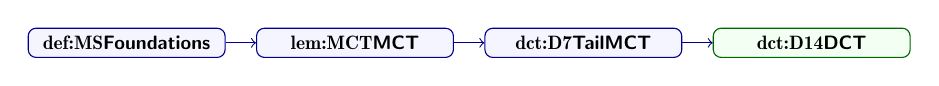
\begin{tikzpicture}
\tikzstyle{dep}=[draw=blue!55!black,fill=blue!4,rounded corners=1mm,
 text width=23mm,text centered,inner sep=1mm]
\tikzstyle{done}=[dep,draw=green!40!black,fill=green!5]
\tikzstyle{flow}=[->,blue!55!black]
\node[dep] (a) at (0.0,0) {\scriptsize \hyperlink{def:MS}{\textsf{Foundations}}};
\node[dep] (w) at (2.9,0) {\scriptsize \hyperlink{lem:MCT}{\textsf{MCT}}};
\node[dep] (p) at (5.8,0) {\scriptsize \hyperlink{dct:D7}{\textsf{TailMCT}}};
\node[done] (m) at (8.7,0) {\scriptsize \hyperlink{dct:D14}{\textsf{DCT}}};
\draw[flow] (a)--(w);
\draw[flow] (w)--(p);
\draw[flow] (p)--(m);
\end{tikzpicture}

\par\vspace{3mm}
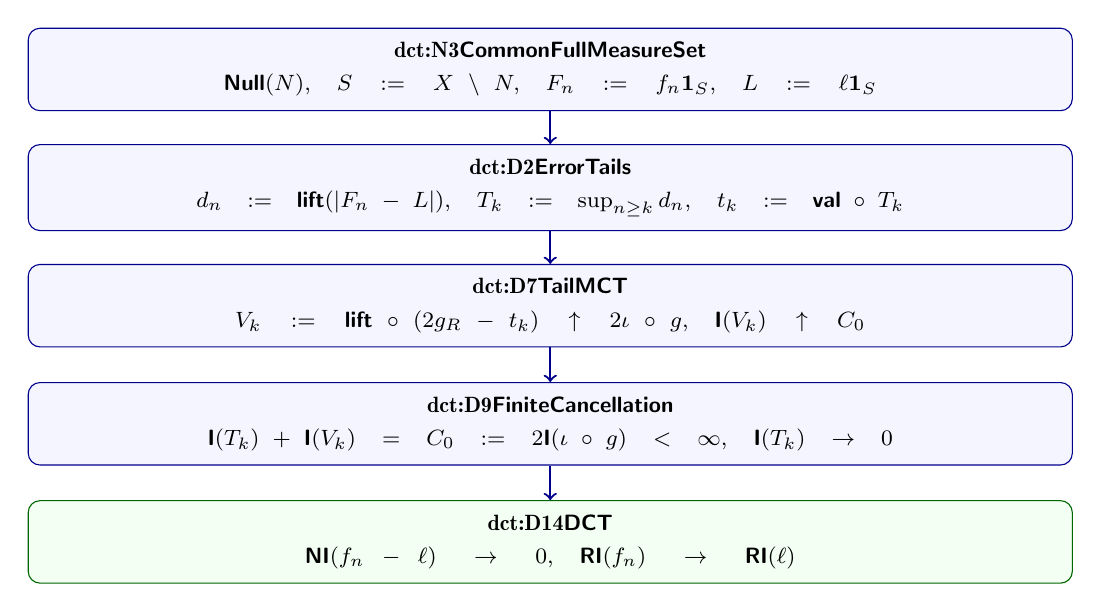
\begin{tikzpicture}
\tikzstyle{dep}=[draw=blue!55!black,fill=blue!4,rounded corners=1.5mm,
 text width=12.9cm,text centered,inner sep=1.8mm]
\tikzstyle{done}=[dep,draw=green!40!black,fill=green!5]
\tikzstyle{flow}=[->,thick,blue!55!black]
\node[dep] (ap) at (0,-0.0) {\footnotesize
\hyperlink{dct:N3}{\textsf{CommonFullMeasureSet}}\\
$\textsf{Null}(N),\quad S:=X\setminus N,\quad
F_n:=f_n\mathbf1_S,\quad L:=\ell\mathbf1_S$};
\node[dep] (win) at (0,-1.5) {\footnotesize
\hyperlink{dct:D2}{\textsf{ErrorTails}}\\
$d_n:=\textsf{lift}(|F_n-L|),\quad
T_k:=\sup_{n\ge k}d_n,\quad t_k:=\textsf{val}\circ T_k$};
\node[dep] (seq) at (0,-3.0) {\footnotesize
\hyperlink{dct:D7}{\textsf{TailMCT}}\\
$V_k:=\textsf{lift}\circ(2g_R-t_k)\uparrow2\iota\circ g,\quad
\textsf{I}(V_k)\uparrow C_0$};
\node[dep] (code) at (0,-4.5) {\footnotesize
\hyperlink{dct:D9}{\textsf{FiniteCancellation}}\\
$\textsf{I}(T_k)+\textsf{I}(V_k)=C_0:=2\textsf{I}(\iota\circ g)<\infty,
\quad\textsf{I}(T_k)\to0$};
\node[done] (result) at (0,-6.0) {\footnotesize
\hyperlink{dct:D14}{\textsf{DCT}}\\
$\textsf{NI}(f_n-\ell)\to0,\quad
\textsf{RI}(f_n)\to\textsf{RI}(\ell)$};
\draw[flow] (ap)--(win);
\draw[flow] (win)--(seq);
\draw[flow] (seq)--(code);
\draw[flow] (code)--(result);
\end{tikzpicture}
\par
\end{minipage}}
\end{figure}

\clearpage
\setstretch{1.2}\pagestyle{plain}\pagenumbering{arabic} %
\hypersetup{pageanchor=true}

\section*{Scope and contribution}

\begin{center}
{\small $\mathsf{MS}(A,\mu ),\quad f:\mathsf{PosNat}\rightarrow X\rightarrow 
\mathsf{Real},\quad \ell :X\rightarrow \mathsf{Real},\quad g:X\rightarrow 
\mathsf{NNReal}.$}

{\small $\mathsf{DCTHyp}(f,\ell ,g)\Rightarrow \mathsf{MR}(\ell )\wedge 
\mathsf{MG}(g)\wedge \mathsf{I}(\iota \circ g)<\infty .$}

{\small $\mathsf{MCT}\wedge \mathsf{IntegralAdd}\wedge \mathsf{%
AENormalization}\Rightarrow \mathsf{TailComplements}\Rightarrow \mathsf{DCT}.
$}

{\small $\mathsf{TypedMathematicalExposition}\neq \mathsf{ExecutableLean}.$}
\end{center}

{\scriptsize \setlength{\parskip}{0pt}\nointerlineskip
\noindent 
\begin{tabular}{|@{}>{\centering\arraybackslash}m{\DCTOneColumnBody}|}
\hline
\hypertarget{theorem:DCT}{$\displaystyle \mathsf{DCT}:\ \forall(X:\mathsf{%
Type})\ (A:\mathsf{Set}(\mathsf{Set}(X)))\ (\mu:\mathsf{Set}(X)\to\mathsf{E}%
),\ \allowbreak\forall(f:\mathsf{PosNat}\to X\to\mathsf{Real})\ (\ell:X\to%
\mathsf{Real})\ (g:X\to\mathsf{NNReal}),\ \allowbreak \mathsf{DCTHyp}%
(f,\ell,g)\ \Longrightarrow\ \allowbreak (\forall n,\ \mathsf{L1}(f_n))\land%
\mathsf{L1}(\ell)\ \land\allowbreak \mathsf{Conv}((\mathsf{NI}%
(f_n-\ell))_n,0)\ \land\allowbreak \mathsf{ConvR}((\mathsf{RI}(f_n))_n,%
\mathsf{RI}(\ell))$} \\ \hline
\end{tabular}%
}

\section{\protect\scriptsize Nonnegative integration}

{\scriptsize \setlength{\parskip}{0pt}\nointerlineskip
\noindent 
\begin{tabular}{|@{}>{\centering\arraybackslash}m{\DCTOneColumnBody}|}
\hline
$\displaystyle \mathsf{NonnegativeFoundations}$ \\ \hline
\end{tabular}%
}

{\scriptsize \setlength{\parskip}{0pt}\nointerlineskip
\noindent 
\begin{tabular}{|@{}>{\centering\arraybackslash}m{\DCTOneColumnBody}|}
\hline
$\displaystyle \mathsf{Context\_0}:=$\par$\displaystyle X:\mathsf{Type}%
,\quad A:\mathsf{Set}(\mathsf{Set}(X)),$\par$\displaystyle \mu:\mathsf{Set}%
(X)\to\mathsf{ENNReal},\quad\mathsf{MS}(A,\mu).$ \\ \hline
\end{tabular}%
}

\subsection{\protect\scriptsize Definitions}

{\scriptsize {\ }}

{\scriptsize \setlength{\parskip}{0pt}\nointerlineskip
\noindent 
\begin{tabular}{|@{}>{\centering\arraybackslash}m{\DCTOneColumnBody}|}
\hline
$\displaystyle \mathsf{Definitions}$ \\ \hline
\end{tabular}%
}

{\scriptsize \setlength{\parskip}{0pt}\nointerlineskip
\noindent 
\begin{tabular}{|@{}>{\centering\arraybackslash}m{0.19251\linewidth}|>{\centering\arraybackslash}m{0.16845\linewidth}|>{\centering\arraybackslash}m{0.53904\linewidth}|}
\hline
$\displaystyle \mathsf{Id}$ & $\displaystyle \mathsf{Kind}$ & $\displaystyle 
\mathsf{Formula}$ \\ \hline
\end{tabular}%
}

{\scriptsize \setlength{\parskip}{0pt}\nointerlineskip
\noindent 
\begin{tabular}{|@{}>{\centering\arraybackslash}m{0.19251\linewidth}|>{\centering\arraybackslash}m{0.16845\linewidth}|>{\centering\arraybackslash}m{0.53904\linewidth}|}
\hline
\hypertarget{def:Types}{$\displaystyle \mathsf{Types}$} & $\displaystyle 
\mathsf{def}$ & $\displaystyle \mathsf{E}:=\mathsf{ENNReal},\quad\mathsf{%
ENNReal}:=\mathsf{WithTop}(\mathsf{NNReal}),$\par$\displaystyle \mathsf{%
PosNat}:=\{n:\mathsf{Nat}\mid 0<n\},$\par$\displaystyle \mathsf{F}:=X\to%
\mathsf{E}.$\par$\displaystyle \mathsf{NNReal}\hookrightarrow\mathsf{E}.$ \\ 
\hline
\end{tabular}%
}

{\scriptsize \setlength{\parskip}{0pt}\nointerlineskip
\noindent 
\begin{tabular}{|@{}>{\centering\arraybackslash}m{0.19251\linewidth}|>{\centering\arraybackslash}m{0.16845\linewidth}|>{\centering\arraybackslash}m{0.53904\linewidth}|}
\hline
\hypertarget{def:MS}{$\displaystyle \mathsf{MS}$} & $\displaystyle \mathsf{%
def}$ & $\displaystyle \mathsf{MS}(A,\mu):\Longleftrightarrow$\par$%
\displaystyle \mathsf{SigmaAlgebra}(A)\land\mathsf{CountAdd}(A,\mu).$ \\ 
\hline
\end{tabular}%
}

{\scriptsize \setlength{\parskip}{0pt}\nointerlineskip
\noindent 
\begin{tabular}{|@{}>{\centering\arraybackslash}m{0.19251\linewidth}|>{\centering\arraybackslash}m{0.16845\linewidth}|>{\centering\arraybackslash}m{0.53904\linewidth}|}
\hline
\hypertarget{def:Meas}{$\displaystyle \mathsf{Meas}$} & $\displaystyle 
\mathsf{def}$ & $\displaystyle \forall h:\mathsf{F},$\par$\displaystyle 
\mathsf{Measurable}(h):\Longleftrightarrow$\par$\displaystyle \forall t:%
\mathsf{NNReal},\ \{x:X\mid h(x)>t\}\in A.$ \\ \hline
\end{tabular}%
}

{\scriptsize \setlength{\parskip}{0pt}\nointerlineskip
\noindent 
\begin{tabular}{|@{}>{\centering\arraybackslash}m{0.19251\linewidth}|>{\centering\arraybackslash}m{0.16845\linewidth}|>{\centering\arraybackslash}m{0.53904\linewidth}|}
\hline
\hypertarget{def:Part}{$\displaystyle \mathsf{Part}$} & $\displaystyle 
\mathsf{def}$ & $\displaystyle r:\mathsf{PosNat},\ P:\mathsf{Fin}(r)\to%
\mathsf{Set}(X),$\par$\displaystyle \mathsf{Part}(P):\Longleftrightarrow$\par%
$\displaystyle (\forall i:\mathsf{Fin}(r),\ P_i\in A)$\par$\displaystyle %
\land\ (\bigcup_{i<r}P_i=X)$\par$\displaystyle \land\ (\forall i,j:\mathsf{%
Fin}(r),$\par$\displaystyle i\ne j\Rightarrow P_i\cap P_j=\varnothing).$ \\ 
\hline
\end{tabular}%
}

{\scriptsize \setlength{\parskip}{0pt}\nointerlineskip
\noindent 
\begin{tabular}{|@{}>{\centering\arraybackslash}m{0.19251\linewidth}|>{\centering\arraybackslash}m{0.16845\linewidth}|>{\centering\arraybackslash}m{0.53904\linewidth}|}
\hline
\hypertarget{def:Rep}{$\displaystyle \mathsf{Rep}$} & $\displaystyle \mathsf{%
def}$ & $\displaystyle s:\mathsf{F},\quad r:\mathsf{PosNat},$\par$%
\displaystyle a:\mathsf{Fin}(r)\to\mathsf{NNReal},\quad P:\mathsf{Fin}(r)\to%
\mathsf{Set}(X),$\par$\displaystyle \mathsf{Rep}(s;r,a,P):\Longleftrightarrow
$\par$\displaystyle \mathsf{Part}(P)\land$\par$\displaystyle s=\lambda x:X,\
\sum_{i<r}a_i\mathbf{1}_{P_i}(x).$ \\ \hline
\end{tabular}%
}

{\scriptsize \setlength{\parskip}{0pt}\nointerlineskip
\noindent 
\begin{tabular}{|@{}>{\centering\arraybackslash}m{0.19251\linewidth}|>{\centering\arraybackslash}m{0.16845\linewidth}|>{\centering\arraybackslash}m{0.53904\linewidth}|}
\hline
\hypertarget{def:Simple}{$\displaystyle \mathsf{Simple}$} & $\displaystyle 
\mathsf{def}$ & $\displaystyle \mathsf{Simple}(s):\Longleftrightarrow$\par$%
\displaystyle \exists r:\mathsf{PosNat},\ \exists a:\mathsf{Fin}(r)\to%
\mathsf{NNReal},$\par$\displaystyle \exists P:\mathsf{Fin}(r)\to\mathsf{Set}%
(X),$\par$\displaystyle \mathsf{Rep}(s;r,a,P).$\par$\displaystyle \mathsf{S}%
_A:=\{s:\mathsf{F}\mid\mathsf{Simple}(s)\}.$ \\ \hline
\end{tabular}%
}

{\scriptsize \setlength{\parskip}{0pt}\nointerlineskip
\noindent 
\begin{tabular}{|@{}>{\centering\arraybackslash}m{0.19251\linewidth}|>{\centering\arraybackslash}m{0.16845\linewidth}|>{\centering\arraybackslash}m{0.53904\linewidth}|}
\hline
\hypertarget{def:J}{$\displaystyle \mathsf{J}$} & $\displaystyle \mathsf{def}
$ & $\displaystyle \mathsf{Rep}(s;r,a,P)\ \Longrightarrow$\par$\displaystyle 
\mathsf{J}(s):=\sum_{i<r}a_i\mu(P_i).$ \\ \hline
\end{tabular}%
}

{\scriptsize \setlength{\parskip}{0pt}\nointerlineskip
\noindent 
\begin{tabular}{|@{}>{\centering\arraybackslash}m{0.19251\linewidth}|>{\centering\arraybackslash}m{0.16845\linewidth}|>{\centering\arraybackslash}m{0.53904\linewidth}|}
\hline
\hypertarget{def:I}{$\displaystyle \mathsf{I}$} & $\displaystyle \mathsf{def}
$ & $\displaystyle \mathsf{I}(h):=\sup\{\mathsf{J}(s)\mid$\par$\displaystyle %
s:\mathsf{S}_A,\ s\le h\},$\par$\displaystyle \int_Xh\,d\mu:=\mathsf{I}(h),$%
\par$\displaystyle h\le v:\Longleftrightarrow\forall x:X,\ h(x)\le v(x).$ \\ 
\hline
\end{tabular}%
}

{\scriptsize \setlength{\parskip}{0pt}\nointerlineskip
\noindent 
\begin{tabular}{|@{}>{\centering\arraybackslash}m{0.19251\linewidth}|>{\centering\arraybackslash}m{0.16845\linewidth}|>{\centering\arraybackslash}m{0.53904\linewidth}|}
\hline
\hypertarget{def:Up}{$\displaystyle \mathsf{Up}$} & $\displaystyle \mathsf{%
def}$ & $\displaystyle Y:\mathsf{Type},\quad[\mathsf{CompleteLattice}(Y)],$%
\par$\displaystyle u:\mathsf{PosNat}\to Y,\quad v:Y,$\par$\displaystyle 
\mathsf{Mono}(u):\Longleftrightarrow$\par$\displaystyle \forall k:\mathsf{%
PosNat},\ u_k\le u_{k+1},$\par$\displaystyle u\uparrow v:\Longleftrightarrow%
\mathsf{Mono}(u)\land v=\sup_k u_k,$\par$\displaystyle E_k\uparrow
E:\Longleftrightarrow$\par$\displaystyle (\forall k:\mathsf{PosNat},\
E_k\subseteq E_{k+1})$\par$\displaystyle \land\ \bigcup_k E_k=E.$ \\ \hline
\end{tabular}%
}

{\scriptsize \setlength{\parskip}{0pt}\nointerlineskip
\noindent 
\begin{tabular}{|@{}>{\centering\arraybackslash}m{0.19251\linewidth}|>{\centering\arraybackslash}m{0.16845\linewidth}|>{\centering\arraybackslash}m{0.53904\linewidth}|}
\hline
\hypertarget{def:Limit}{$\displaystyle \mathsf{Limit}$} & $\displaystyle 
\mathsf{def}$ & $\displaystyle a:\mathsf{PosNat}\to\mathsf{E},\ L:\mathsf{E},
$\par$\displaystyle \mathsf{Conv}(a,L):\Longleftrightarrow$\par$%
\displaystyle \bigl(L<\infty\Rightarrow$\par$\displaystyle %
\forall\varepsilon:\mathsf{NNReal},\ \varepsilon>0\Rightarrow$\par$%
\displaystyle \exists K:\mathsf{PosNat},\ \forall k\ge K,$\par$\displaystyle %
a_k<L+\varepsilon\land L<a_k+\varepsilon\bigr)$\par$\displaystyle \land\ %
\bigl(L=\infty\Rightarrow$\par$\displaystyle \forall R:\mathsf{NNReal},\
\exists K:\mathsf{PosNat},$\par$\displaystyle \forall k\ge K,\ R<a_k\bigr).$
\\ \hline
\end{tabular}%
}

{\scriptsize \ }

\subsection{\protect\scriptsize Axioms}

{\scriptsize {\ }}

{\scriptsize \setlength{\parskip}{0pt}\nointerlineskip
\noindent 
\begin{tabular}{|@{}>{\centering\arraybackslash}m{\DCTOneColumnBody}|}
\hline
$\displaystyle \mathsf{Axioms}$ \\ \hline
\end{tabular}%
}

{\scriptsize \setlength{\parskip}{0pt}\nointerlineskip
\noindent 
\begin{tabular}{|@{}>{\centering\arraybackslash}m{0.19251\linewidth}|>{\centering\arraybackslash}m{0.16845\linewidth}|>{\centering\arraybackslash}m{0.53904\linewidth}|}
\hline
$\displaystyle \mathsf{Id}$ & $\displaystyle \mathsf{Kind}$ & $\displaystyle 
\mathsf{Formula}$ \\ \hline
\end{tabular}%
}

{\scriptsize \setlength{\parskip}{0pt}\nointerlineskip
\noindent 
\begin{tabular}{|@{}>{\centering\arraybackslash}m{0.19251\linewidth}|>{\centering\arraybackslash}m{0.16845\linewidth}|>{\centering\arraybackslash}m{0.53904\linewidth}|}
\hline
\hypertarget{ax:Sigma}{$\displaystyle \mathsf{Sigma}$} & $\displaystyle 
\mathsf{axiom}$ & $\displaystyle \mathsf{SigmaAlgebra}(A):\Longleftrightarrow
$\par$\displaystyle X\in A\ \land$\par$\displaystyle (\forall B:\mathsf{Set}%
(X),\ B\in A\Rightarrow X\setminus B\in A)$\par$\displaystyle \land\
(\forall B:\mathsf{PosNat}\to\mathsf{Set}(X),$\par$\displaystyle (\forall n:%
\mathsf{PosNat},\ B_n\in A)$\par$\displaystyle \Rightarrow\bigcup_n B_n\in
A).$ \\ \hline
\end{tabular}%
}

{\scriptsize \setlength{\parskip}{0pt}\nointerlineskip
\noindent 
\begin{tabular}{|@{}>{\centering\arraybackslash}m{0.19251\linewidth}|>{\centering\arraybackslash}m{0.16845\linewidth}|>{\centering\arraybackslash}m{0.53904\linewidth}|}
\hline
\hypertarget{ax:Measure}{$\displaystyle \mathsf{Measure}$} & $\displaystyle 
\mathsf{axiom}$ & $\displaystyle \mathsf{CountAdd}(A,\mu):\Longleftrightarrow
$\par$\displaystyle \mu(\varnothing)=0\ \land$\par$\displaystyle \forall B:%
\mathsf{PosNat}\to\mathsf{Set}(X),$\par$\displaystyle \bigl((\forall n:%
\mathsf{PosNat},\ B_n\in A)$\par$\displaystyle \land\ (\forall i,j:\mathsf{%
PosNat},$\par$\displaystyle i\ne j\Rightarrow B_i\cap B_j=\varnothing)\bigr)$%
\par$\displaystyle \Rightarrow\mu(\bigcup_n B_n)=\sum_{n\ge1}\mu(B_n).$ \\ 
\hline
\end{tabular}%
}

{\scriptsize \setlength{\parskip}{0pt}\nointerlineskip
\noindent 
\begin{tabular}{|@{}>{\centering\arraybackslash}m{0.19251\linewidth}|>{\centering\arraybackslash}m{0.16845\linewidth}|>{\centering\arraybackslash}m{0.53904\linewidth}|}
\hline
\hypertarget{ax:Order}{$\displaystyle \mathsf{Order}$} & $\displaystyle 
\mathsf{axiom}$ & $\displaystyle \mathsf{LinearOrderedField}(\mathsf{Real}),$%
\par$\displaystyle \mathsf{Archimedean}(\mathsf{Real}),$\par$\displaystyle 
\mathsf{ConditionallyCompleteLinearOrder}(\mathsf{Real}),$\par$\displaystyle 
\mathsf{NNReal}=\{x:\mathsf{Real}\mid0\le x\},$\par$\displaystyle \mathsf{E}=%
\mathsf{WithTop}(\mathsf{NNReal}),$\par$\displaystyle \mathsf{%
CompleteLinearOrder}(\mathsf{E}),$\par$\displaystyle 0\cdot\infty=0,\quad%
\infty+z=\infty,$\par$\displaystyle \sum_{n\ge1}z_n:=\sup_k\sum_{n=1}^kz_n,$%
\par$\displaystyle \forall\varepsilon:\mathsf{NNReal},\
\varepsilon>0\Rightarrow$\par$\displaystyle \exists j:\mathsf{PosNat},\
1/j<\varepsilon.$ \\ \hline
\end{tabular}%
}

{\scriptsize \ }

\subsection{\protect\scriptsize Logical rules}

{\scriptsize {\ }}

{\scriptsize \setlength{\parskip}{0pt}\nointerlineskip
\noindent 
\begin{tabular}{|@{}>{\centering\arraybackslash}m{\DCTOneColumnBody}|}
\hline
$\displaystyle \mathsf{Logic}$ \\ \hline
\end{tabular}%
}

{\scriptsize \setlength{\parskip}{0pt}\nointerlineskip
\noindent 
\begin{tabular}{|@{}>{\centering\arraybackslash}m{0.19251\linewidth}|>{\centering\arraybackslash}m{0.16845\linewidth}|>{\centering\arraybackslash}m{0.53904\linewidth}|}
\hline
$\displaystyle \mathsf{Id}$ & $\displaystyle \mathsf{Symbol}$ & $%
\displaystyle \mathsf{Formula}$ \\ \hline
\end{tabular}%
}

{\scriptsize \setlength{\parskip}{0pt}\nointerlineskip
\noindent 
\begin{tabular}{|@{}>{\centering\arraybackslash}m{0.19251\linewidth}|>{\centering\arraybackslash}m{0.16845\linewidth}|>{\centering\arraybackslash}m{0.53904\linewidth}|}
\hline
\hypertarget{rule:AllI}{$\displaystyle \mathsf{AllI}$} & $\displaystyle %
\forall I$ & \rule[-3.3ex]{0pt}{7.8ex}$\displaystyle \dfrac{\Gamma\vdash
P(x)\quad x\notin\mathsf{FV}(\Gamma)}{\Gamma\vdash\forall x\,P(x)}$ \\ \hline
\end{tabular}%
}

{\scriptsize \setlength{\parskip}{0pt}\nointerlineskip
\noindent 
\begin{tabular}{|@{}>{\centering\arraybackslash}m{0.19251\linewidth}|>{\centering\arraybackslash}m{0.16845\linewidth}|>{\centering\arraybackslash}m{0.53904\linewidth}|}
\hline
\hypertarget{rule:AllE}{$\displaystyle \mathsf{AllE}$} & $\displaystyle %
\forall E$ & \rule[-3.3ex]{0pt}{7.8ex}$\displaystyle \dfrac{%
\Gamma\vdash\forall x\,P(x)}{\Gamma\vdash P(a)}$ \\ \hline
\end{tabular}%
}

{\scriptsize \setlength{\parskip}{0pt}\nointerlineskip
\noindent 
\begin{tabular}{|@{}>{\centering\arraybackslash}m{0.19251\linewidth}|>{\centering\arraybackslash}m{0.16845\linewidth}|>{\centering\arraybackslash}m{0.53904\linewidth}|}
\hline
\hypertarget{rule:AndI}{$\displaystyle \mathsf{AndI}$} & $\displaystyle %
\wedge I$ & \rule[-3.3ex]{0pt}{7.8ex}$\displaystyle \dfrac{\Gamma\vdash
P\quad\Gamma\vdash Q}{\Gamma\vdash P\land Q}$ \\ \hline
\end{tabular}%
}

{\scriptsize \setlength{\parskip}{0pt}\nointerlineskip
\noindent 
\begin{tabular}{|@{}>{\centering\arraybackslash}m{0.19251\linewidth}|>{\centering\arraybackslash}m{0.16845\linewidth}|>{\centering\arraybackslash}m{0.53904\linewidth}|}
\hline
\hypertarget{rule:AndE}{$\displaystyle \mathsf{AndE}$} & $\displaystyle %
\wedge E$ & \rule[-3.3ex]{0pt}{7.8ex}$\displaystyle \dfrac{\Gamma\vdash
P\land Q}{\Gamma\vdash P}\quad\dfrac{\Gamma\vdash P\land Q}{\Gamma\vdash Q}$
\\ \hline
\end{tabular}%
}

{\scriptsize \setlength{\parskip}{0pt}\nointerlineskip
\noindent 
\begin{tabular}{|@{}>{\centering\arraybackslash}m{0.19251\linewidth}|>{\centering\arraybackslash}m{0.16845\linewidth}|>{\centering\arraybackslash}m{0.53904\linewidth}|}
\hline
\hypertarget{rule:ImpI}{$\displaystyle \mathsf{ImpI}$} & $\displaystyle \to I
$ & \rule[-3.3ex]{0pt}{7.8ex}$\displaystyle \dfrac{\Gamma,P\vdash Q}{%
\Gamma\vdash P\to Q}$ \\ \hline
\end{tabular}%
}

{\scriptsize \setlength{\parskip}{0pt}\nointerlineskip
\noindent 
\begin{tabular}{|@{}>{\centering\arraybackslash}m{0.19251\linewidth}|>{\centering\arraybackslash}m{0.16845\linewidth}|>{\centering\arraybackslash}m{0.53904\linewidth}|}
\hline
\hypertarget{rule:MP}{$\displaystyle \mathsf{MP}$} & $\displaystyle \to E$ & 
\rule[-3.3ex]{0pt}{7.8ex}$\displaystyle \dfrac{\Gamma\vdash
P\quad\Gamma\vdash P\to Q}{\Gamma\vdash Q}$ \\ \hline
\end{tabular}%
}

{\scriptsize \setlength{\parskip}{0pt}\nointerlineskip
\noindent 
\begin{tabular}{|@{}>{\centering\arraybackslash}m{0.19251\linewidth}|>{\centering\arraybackslash}m{0.16845\linewidth}|>{\centering\arraybackslash}m{0.53904\linewidth}|}
\hline
\hypertarget{rule:ExistsI}{$\displaystyle \mathsf{ExistsI}$} & $%
\displaystyle \exists I$ & \rule[-3.3ex]{0pt}{7.8ex}$\displaystyle \dfrac{%
\Gamma\vdash P(a)}{\Gamma\vdash\exists x\,P(x)}$ \\ \hline
\end{tabular}%
}

{\scriptsize \setlength{\parskip}{0pt}\nointerlineskip
\noindent 
\begin{tabular}{|@{}>{\centering\arraybackslash}m{0.19251\linewidth}|>{\centering\arraybackslash}m{0.16845\linewidth}|>{\centering\arraybackslash}m{0.53904\linewidth}|}
\hline
\hypertarget{rule:ExistsE}{$\displaystyle \mathsf{ExistsE}$} & $%
\displaystyle \exists E$ & \rule[-3.3ex]{0pt}{7.8ex}$\displaystyle \dfrac{%
\Gamma\vdash\exists xP(x)\quad\Gamma,P(y)\vdash Q}{\Gamma\vdash Q}$\par$%
\displaystyle y\notin\mathsf{FV}(\Gamma,Q).$ \\ \hline
\end{tabular}%
}

{\scriptsize \setlength{\parskip}{0pt}\nointerlineskip
\noindent 
\begin{tabular}{|@{}>{\centering\arraybackslash}m{0.19251\linewidth}|>{\centering\arraybackslash}m{0.16845\linewidth}|>{\centering\arraybackslash}m{0.53904\linewidth}|}
\hline
\hypertarget{rule:Eq}{$\displaystyle \mathsf{Eq}$} & $\displaystyle =E$ & 
\rule[-3.3ex]{0pt}{7.8ex}$\displaystyle \dfrac{\Gamma\vdash
a=b\quad\Gamma\vdash P(a)}{\Gamma\vdash P(b)}$ \\ \hline
\end{tabular}%
}

{\scriptsize \setlength{\parskip}{0pt}\nointerlineskip
\noindent 
\begin{tabular}{|@{}>{\centering\arraybackslash}m{0.19251\linewidth}|>{\centering\arraybackslash}m{0.16845\linewidth}|>{\centering\arraybackslash}m{0.53904\linewidth}|}
\hline
\hypertarget{rule:Cases}{$\displaystyle \mathsf{Cases}$} & $\displaystyle %
\vee E$ & \rule[-3.3ex]{0pt}{7.8ex}$\displaystyle \dfrac{\Gamma\vdash P\lor
Q\quad\Gamma,P\vdash R\quad\Gamma,Q\vdash R}{\Gamma\vdash R}$ \\ \hline
\end{tabular}%
}

{\scriptsize \ }

\subsection{\protect\scriptsize Lemmas}

{\scriptsize {\ }}

{\scriptsize \setlength{\parskip}{0pt}\nointerlineskip
\noindent 
\begin{tabular}{|@{}>{\centering\arraybackslash}m{\DCTOneColumnBody}|}
\hline
$\displaystyle \mathsf{Lemmas}$ \\ \hline
\end{tabular}%
}

{\scriptsize \setlength{\parskip}{0pt}\nointerlineskip
\noindent 
\begin{tabular}{|@{}>{\centering\arraybackslash}m{0.19251\linewidth}|>{\centering\arraybackslash}m{0.16845\linewidth}|>{\centering\arraybackslash}m{0.53904\linewidth}|}
\hline
$\displaystyle \mathsf{Id}$ & $\displaystyle \mathsf{Proof}$ & $%
\displaystyle \mathsf{Formula}$ \\ \hline
\end{tabular}%
}

{\scriptsize \setlength{\parskip}{0pt}\nointerlineskip
\noindent 
\begin{tabular}{|@{}>{\centering\arraybackslash}m{0.19251\linewidth}|>{\centering\arraybackslash}m{0.16845\linewidth}|>{\centering\arraybackslash}m{0.53904\linewidth}|}
\hline
\hypertarget{lem:Order}{$\displaystyle \mathsf{Order}$} & \hyperlink{proof:O4}%
{$\displaystyle \mathsf{O4}$} & $\displaystyle \forall a:\mathsf{PosNat}\to%
\mathsf{E},$\par$\displaystyle \mathsf{Mono}(a)\Rightarrow\mathsf{Conv}%
(a,\sup_k a_k).$ \\ \hline
\end{tabular}%
}

{\scriptsize \setlength{\parskip}{0pt}\nointerlineskip
\noindent 
\begin{tabular}{|@{}>{\centering\arraybackslash}m{0.19251\linewidth}|>{\centering\arraybackslash}m{0.16845\linewidth}|>{\centering\arraybackslash}m{0.53904\linewidth}|}
\hline
\hypertarget{lem:Continuity}{$\displaystyle \mathsf{Continuity}$} & 
\hyperlink{proof:C6}{$\displaystyle \mathsf{C6}$} & $\displaystyle E_k\in
A,\ E_k\uparrow E$\par$\displaystyle \Rightarrow\mu(E)=\sup_k\mu(E_k)$\par$%
\displaystyle \land\mathsf{Conv}((\mu(E_k))_k,\mu(E)).$ \\ \hline
\end{tabular}%
}

{\scriptsize \setlength{\parskip}{0pt}\nointerlineskip
\noindent 
\begin{tabular}{|@{}>{\centering\arraybackslash}m{0.19251\linewidth}|>{\centering\arraybackslash}m{0.16845\linewidth}|>{\centering\arraybackslash}m{0.53904\linewidth}|}
\hline
\hypertarget{lem:Simple}{$\displaystyle \mathsf{Simple}$} & \hyperlink{proof:J5}%
{$\displaystyle \mathsf{J5}$} & $\displaystyle \mathsf{Rep}(s;r,a,P)\land%
\mathsf{Rep}(s;q,b,Q)$\par$\displaystyle \Rightarrow\sum_i
a_i\mu(P_i)=\sum_j b_j\mu(Q_j),$\par$\displaystyle s,t:\mathsf{S}_A,\ s\le
t\Rightarrow\mathsf{J}(s)\le\mathsf{J}(t),$\par$\displaystyle c:\mathsf{%
NNReal}\Rightarrow\mathsf{J}(cs)=c\mathsf{J}(s).$ \\ \hline
\end{tabular}%
}

{\scriptsize \setlength{\parskip}{0pt}\nointerlineskip
\noindent 
\begin{tabular}{|@{}>{\centering\arraybackslash}m{0.19251\linewidth}|>{\centering\arraybackslash}m{0.16845\linewidth}|>{\centering\arraybackslash}m{0.53904\linewidth}|}
\hline
\hypertarget{lem:Finite}{$\displaystyle \mathsf{Finite}$} & \hyperlink{proof:D4}%
{$\displaystyle \mathsf{D4}$} & $\displaystyle z_{ik}\uparrow z_i\ (i:%
\mathsf{Fin}(r))$\par$\displaystyle \Rightarrow\sup_k\sum_{i<r}z_{ik}=%
\sum_{i<r}z_i.$ \\ \hline
\end{tabular}%
}

{\scriptsize \setlength{\parskip}{0pt}\nointerlineskip
\noindent 
\begin{tabular}{|@{}>{\centering\arraybackslash}m{0.19251\linewidth}|>{\centering\arraybackslash}m{0.16845\linewidth}|>{\centering\arraybackslash}m{0.53904\linewidth}|}
\hline
\hypertarget{lem:Integral}{$\displaystyle \mathsf{Integral}$} & \hyperlink{proof:I3}%
{$\displaystyle \mathsf{I3}$} & $\displaystyle h\le v\Rightarrow\mathsf{I}%
(h)\le\mathsf{I}(v),$\par$\displaystyle s:\mathsf{S}_A\Rightarrow\mathsf{I}%
(s)=\mathsf{J}(s).$ \\ \hline
\end{tabular}%
}

{\scriptsize \setlength{\parskip}{0pt}\nointerlineskip
\noindent 
\begin{tabular}{|@{}>{\centering\arraybackslash}m{0.19251\linewidth}|>{\centering\arraybackslash}m{0.16845\linewidth}|>{\centering\arraybackslash}m{0.53904\linewidth}|}
\hline
\hypertarget{lem:Meas}{$\displaystyle \mathsf{Meas}$} & \hyperlink{proof:P4}{%
$\displaystyle \mathsf{P4}$} & $\displaystyle (\forall n:\mathsf{PosNat},\ 
\mathsf{Measurable}(h_n))$\par$\displaystyle \Rightarrow\mathsf{Measurable}%
(\inf_n h_n)$\par$\displaystyle \land\mathsf{Measurable}(\sup_n h_n).$ \\ 
\hline
\end{tabular}%
}

{\scriptsize \setlength{\parskip}{0pt}\nointerlineskip
\noindent 
\begin{tabular}{|@{}>{\centering\arraybackslash}m{0.19251\linewidth}|>{\centering\arraybackslash}m{0.16845\linewidth}|>{\centering\arraybackslash}m{0.53904\linewidth}|}
\hline
\hypertarget{lem:Restriction}{$\displaystyle \mathsf{Restriction}$} & 
\hyperlink{proof:T2}{$\displaystyle \mathsf{T2}$} & $\displaystyle E_k\in
A,\ E_k\uparrow X,\ s:\mathsf{S}_A$\par$\displaystyle \Rightarrow\sup_k%
\mathsf{J}(s\mathbf{1}_{E_k})=\mathsf{J}(s).$ \\ \hline
\end{tabular}%
}

{\scriptsize \setlength{\parskip}{0pt}\nointerlineskip
\noindent 
\begin{tabular}{|@{}>{\centering\arraybackslash}m{0.19251\linewidth}|>{\centering\arraybackslash}m{0.16845\linewidth}|>{\centering\arraybackslash}m{0.53904\linewidth}|}
\hline
\hypertarget{lem:MonoIntegralConv}{$\displaystyle \mathsf{MonoIntegralConv}$}
& \hyperlink{proof:L3}{$\displaystyle \mathsf{L3}$} & $\displaystyle \mathsf{%
Mono}(u)\land(\forall k,\ \mathsf{Measurable}(u_k))$\par$\displaystyle %
\Rightarrow\mathsf{Conv}((\mathsf{I}(u_k))_k,\sup_k\mathsf{I}(u_k)).$ \\ 
\hline
\end{tabular}%
}

{\scriptsize \setlength{\parskip}{0pt}\nointerlineskip
\noindent 
\begin{tabular}{|@{}>{\centering\arraybackslash}m{0.19251\linewidth}|>{\centering\arraybackslash}m{0.16845\linewidth}|>{\centering\arraybackslash}m{0.53904\linewidth}|}
\hline
\hypertarget{lem:MCT}{$\displaystyle \mathsf{MCT}$} & \hyperlink{proof:M13}{$%
\displaystyle \mathsf{M13}$} & $\displaystyle u_k\uparrow v\land(\forall k,\ 
\mathsf{Measurable}(u_k))$\par$\displaystyle \Rightarrow\mathsf{I}(v)=\sup_k%
\mathsf{I}(u_k)$\par$\displaystyle \land\mathsf{Conv}((\mathsf{I}(u_k))_k,%
\mathsf{I}(v)).$ \\ \hline
\end{tabular}%
}

{\scriptsize \ }

\subsection{\protect\scriptsize Supporting proofs}

{\scriptsize {\ }}

{\scriptsize \setlength{\parskip}{0pt}\nointerlineskip
\noindent 
\begin{tabular}{|@{}>{\centering\arraybackslash}m{\DCTOneColumnBody}|}
\hline
$\displaystyle \mathsf{Proofs}$ \\ \hline
\end{tabular}%
}

{\scriptsize \setlength{\parskip}{0pt}\nointerlineskip
\noindent 
\begin{tabular}{|@{}>{\centering\arraybackslash}m{0.10658\linewidth}|>{\centering\arraybackslash}m{0.03553\linewidth}|>{\centering\arraybackslash}m{0.52105\linewidth}|>{\centering\arraybackslash}m{0.23684\linewidth}|}
\hline
$\displaystyle \mathsf{Block}$ & $\displaystyle \mathsf{Step}$ & $%
\displaystyle \mathsf{Formula}$ & $\displaystyle \mathsf{Dependencies}$ \\ 
\hline
\end{tabular}%
}

\subsubsection{\protect\scriptsize Extended-real order}

{\scriptsize \setlength{\parskip}{0pt}\nointerlineskip
\noindent 
\begin{tabular}{|@{}>{\centering\arraybackslash}m{\DCTOneColumnBody}|}
\hline
$\displaystyle \mathsf{Context\_O}:=$\par$\displaystyle a:\mathsf{PosNat}\to%
\mathsf{E},\quad\mathsf{Mono}(a).$ \\ \hline
\end{tabular}%
}

{\scriptsize \setlength{\parskip}{0pt}\nointerlineskip
\noindent 
\begin{tabular}{|@{}>{\centering\arraybackslash}m{0.10658\linewidth}|>{\centering\arraybackslash}m{0.03553\linewidth}|>{\centering\arraybackslash}m{0.52105\linewidth}|>{\centering\arraybackslash}m{0.23684\linewidth}|}
\hline
\hypertarget{proof:O1}{$\displaystyle \mathsf{O}$} & $\displaystyle 1$ & $%
\displaystyle L:=\sup_{k\ge1}a_k\in\mathsf{E},$\par$\displaystyle \forall k:%
\mathsf{PosNat},\ a_k\le L.$\par$\displaystyle \mathsf{Rule}:\ \sup$ & 
\hyperlink{ax:Order}{$\displaystyle \mathsf{Order}$} \\ \hline
\end{tabular}%
}

{\scriptsize \setlength{\parskip}{0pt}\nointerlineskip
\noindent 
\begin{tabular}{|@{}>{\centering\arraybackslash}m{0.10658\linewidth}|>{\centering\arraybackslash}m{0.03553\linewidth}|>{\centering\arraybackslash}m{0.52105\linewidth}|>{\centering\arraybackslash}m{0.23684\linewidth}|}
\hline
\hypertarget{proof:O2}{$\displaystyle \mathsf{O}$} & $\displaystyle 2$ & $%
\displaystyle L<\infty,\quad0<\varepsilon:\mathsf{NNReal},$\par$%
\displaystyle L<\varepsilon\Rightarrow L<a_1+\varepsilon,$\par$\displaystyle %
\varepsilon\le L\Rightarrow L-\varepsilon<L$\par$\displaystyle %
\Rightarrow\exists K:\mathsf{PosNat},\ L-\varepsilon<a_K,$\par$\displaystyle %
\Rightarrow\exists K:\mathsf{PosNat},\ \forall k\ge K,$\par$\displaystyle %
a_k<L+\varepsilon\land L<a_k+\varepsilon.$\par$\displaystyle \mathsf{Rule}:\
\sup$ & \hyperlink{proof:O1}{$\displaystyle \mathsf{O1}$}, \hyperlink{ax:Order}%
{$\displaystyle \mathsf{Order}$} \\ \hline
\end{tabular}%
}

{\scriptsize \setlength{\parskip}{0pt}\nointerlineskip
\noindent 
\begin{tabular}{|@{}>{\centering\arraybackslash}m{0.10658\linewidth}|>{\centering\arraybackslash}m{0.03553\linewidth}|>{\centering\arraybackslash}m{0.52105\linewidth}|>{\centering\arraybackslash}m{0.23684\linewidth}|}
\hline
\hypertarget{proof:O3}{$\displaystyle \mathsf{O}$} & $\displaystyle 3$ & $%
\displaystyle L=\infty\Rightarrow\forall R:\mathsf{NNReal},$\par$%
\displaystyle \exists K:\mathsf{PosNat},\ R<a_K$\par$\displaystyle %
\Rightarrow\forall k\ge K,\ R<a_k.$\par$\displaystyle \mathsf{Rule}:\ \sup$
& \hyperlink{proof:O1}{$\displaystyle \mathsf{O1}$}, \hyperlink{ax:Order}{$%
\displaystyle \mathsf{Order}$} \\ \hline
\end{tabular}%
}

{\scriptsize \setlength{\parskip}{0pt}\nointerlineskip
\noindent 
\begin{tabular}{|@{}>{\centering\arraybackslash}m{0.10658\linewidth}|>{\centering\arraybackslash}m{0.03553\linewidth}|>{\centering\arraybackslash}m{0.52105\linewidth}|>{\centering\arraybackslash}m{0.23684\linewidth}|}
\hline
\hypertarget{proof:O4}{$\displaystyle \mathsf{O}$} & $\displaystyle 4$ & $%
\displaystyle \mathsf{Conv}(a,\sup_k a_k).$\par$\displaystyle \mathsf{Rule}%
:\ \lor E$ & \hyperlink{proof:O2}{$\displaystyle \mathsf{O2}$}, \hyperlink{proof:O3}%
{$\displaystyle \mathsf{O3}$}, \hyperlink{def:Limit}{$\displaystyle \mathsf{%
Limit}$} \\ \hline
\end{tabular}%
}

\subsubsection{\protect\scriptsize Continuity from below}

{\scriptsize \setlength{\parskip}{0pt}\nointerlineskip
\noindent 
\begin{tabular}{|@{}>{\centering\arraybackslash}m{\DCTOneColumnBody}|}
\hline
$\displaystyle \mathsf{Context\_C}:=$\par$\displaystyle E:\mathsf{PosNat}\to%
\mathsf{Set}(X),$\par$\displaystyle (\forall k:\mathsf{PosNat},\ E_k\in A)$%
\par$\displaystyle \land(\forall k:\mathsf{PosNat},\ E_k\subseteq E_{k+1}).$
\\ \hline
\end{tabular}%
}

{\scriptsize \setlength{\parskip}{0pt}\nointerlineskip
\noindent 
\begin{tabular}{|@{}>{\centering\arraybackslash}m{0.10658\linewidth}|>{\centering\arraybackslash}m{0.03553\linewidth}|>{\centering\arraybackslash}m{0.52105\linewidth}|>{\centering\arraybackslash}m{0.23684\linewidth}|}
\hline
\hypertarget{proof:C1}{$\displaystyle \mathsf{C}$} & $\displaystyle 1$ & $%
\displaystyle B:\mathsf{Fin}(r)\to\mathsf{Set}(X),$\par$\displaystyle %
(\forall i<r,\ B_i\in A)\land$\par$\displaystyle (\forall i\ne j,\ B_i\cap
B_j=\varnothing)$\par$\displaystyle \Rightarrow\mu(\bigcup_{i<r}B_i)=%
\sum_{i<r}\mu(B_i),$\par$\displaystyle B_n^\prime:=\mathsf{if}\ n\le r\ 
\mathsf{then}\ B_{n-1}$\par$\displaystyle \mathsf{else}\
\varnothing,\quad\mu(\varnothing)=0.$\par$\displaystyle \mathsf{Rule}:\ \sum$
& \hyperlink{ax:Measure}{$\displaystyle \mathsf{Measure}$} \\ \hline
\end{tabular}%
}

{\scriptsize \setlength{\parskip}{0pt}\nointerlineskip
\noindent 
\begin{tabular}{|@{}>{\centering\arraybackslash}m{0.10658\linewidth}|>{\centering\arraybackslash}m{0.03553\linewidth}|>{\centering\arraybackslash}m{0.52105\linewidth}|>{\centering\arraybackslash}m{0.23684\linewidth}|}
\hline
\hypertarget{proof:C2}{$\displaystyle \mathsf{C}$} & $\displaystyle 2$ & $%
\displaystyle U,V:\mathsf{Set}(X),\ U,V\in A,\ U\subseteq V,$\par$%
\displaystyle V=U\mathbin{\dot\cup}(V\setminus U),$\par$\displaystyle %
\mu(V)=\mu(U)+\mu(V\setminus U)\ge\mu(U).$\par$\displaystyle \mathsf{Rule}:\
\le$ & \hyperlink{proof:C1}{$\displaystyle \mathsf{C1}$}, \hyperlink{ax:Sigma}%
{$\displaystyle \mathsf{Sigma}$} \\ \hline
\end{tabular}%
}

{\scriptsize \setlength{\parskip}{0pt}\nointerlineskip
\noindent 
\begin{tabular}{|@{}>{\centering\arraybackslash}m{0.10658\linewidth}|>{\centering\arraybackslash}m{0.03553\linewidth}|>{\centering\arraybackslash}m{0.52105\linewidth}|>{\centering\arraybackslash}m{0.23684\linewidth}|}
\hline
\hypertarget{proof:C3}{$\displaystyle \mathsf{C}$} & $\displaystyle 3$ & $%
\displaystyle B_1:=E_1,\quad B_{j+1}:=E_{j+1}\setminus E_j,$\par$%
\displaystyle \forall j:\mathsf{PosNat},\ B_j\in A,$\par$\displaystyle %
\forall i,j:\mathsf{PosNat},$\par$\displaystyle i\ne j\Rightarrow B_i\cap
B_j=\varnothing.$\par$\displaystyle \mathsf{Rule}:\ \setminus$ & \hyperlink{ax:Sigma}%
{$\displaystyle \mathsf{Sigma}$} \\ \hline
\end{tabular}%
}

{\scriptsize \setlength{\parskip}{0pt}\nointerlineskip
\noindent 
\begin{tabular}{|@{}>{\centering\arraybackslash}m{0.10658\linewidth}|>{\centering\arraybackslash}m{0.03553\linewidth}|>{\centering\arraybackslash}m{0.52105\linewidth}|>{\centering\arraybackslash}m{0.23684\linewidth}|}
\hline
\hypertarget{proof:C4}{$\displaystyle \mathsf{C}$} & $\displaystyle 4$ & $%
\displaystyle E_k=\mathop{\dot\bigcup}_{j=1}^kB_j,$\par$\displaystyle %
\mu(E_k)=\sum_{j=1}^k\mu(B_j).$\par$\displaystyle \mathsf{Rule}:\ \sum$ & 
\hyperlink{proof:C1}{$\displaystyle \mathsf{C1}$}, \hyperlink{proof:C3}{$%
\displaystyle \mathsf{C3}$} \\ \hline
\end{tabular}%
}

{\scriptsize \setlength{\parskip}{0pt}\nointerlineskip
\noindent 
\begin{tabular}{|@{}>{\centering\arraybackslash}m{0.10658\linewidth}|>{\centering\arraybackslash}m{0.03553\linewidth}|>{\centering\arraybackslash}m{0.52105\linewidth}|>{\centering\arraybackslash}m{0.23684\linewidth}|}
\hline
\hypertarget{proof:C5}{$\displaystyle \mathsf{C}$} & $\displaystyle 5$ & $%
\displaystyle \bigcup_kE_k=\mathop{\dot\bigcup}_{j\ge1}B_j,$\par$%
\displaystyle \mu(\bigcup_kE_k)=\sum_{j\ge1}\mu(B_j)$\par$\displaystyle %
{}=\sup_k\mu(E_k).$\par$\displaystyle \mathsf{Rule}:\ \sup$ & \hyperlink{proof:C3}%
{$\displaystyle \mathsf{C3}$}, \hyperlink{proof:C4}{$\displaystyle \mathsf{C4%
}$}, \hyperlink{ax:Measure}{$\displaystyle \mathsf{Measure}$}, \hyperlink{ax:Order}%
{$\displaystyle \mathsf{Order}$} \\ \hline
\end{tabular}%
}

{\scriptsize \setlength{\parskip}{0pt}\nointerlineskip
\noindent 
\begin{tabular}{|@{}>{\centering\arraybackslash}m{0.10658\linewidth}|>{\centering\arraybackslash}m{0.03553\linewidth}|>{\centering\arraybackslash}m{0.52105\linewidth}|>{\centering\arraybackslash}m{0.23684\linewidth}|}
\hline
\hypertarget{proof:C6}{$\displaystyle \mathsf{C}$} & $\displaystyle 6$ & $%
\displaystyle \mu(E_k)\uparrow\mu(\bigcup_kE_k),$\par$\displaystyle \mathsf{%
Conv}((\mu(E_k))_k,\mu(\bigcup_kE_k)).$\par$\displaystyle \mathsf{Rule}:\
\land I$ & \hyperlink{proof:C2}{$\displaystyle \mathsf{C2}$}, \hyperlink{proof:C5}%
{$\displaystyle \mathsf{C5}$}, \hyperlink{lem:Order}{$\displaystyle \mathsf{%
Order}$} \\ \hline
\end{tabular}%
}

\subsubsection{\protect\scriptsize Simple integration}

{\scriptsize \setlength{\parskip}{0pt}\nointerlineskip
\noindent 
\begin{tabular}{|@{}>{\centering\arraybackslash}m{\DCTOneColumnBody}|}
\hline
$\displaystyle \mathsf{Context\_J}:=$\par$\displaystyle s,t:\mathsf{S}_A,$%
\par$\displaystyle \mathsf{Rep}(s;r,a,P),\quad\mathsf{Rep}(t;q,b,Q).$ \\ 
\hline
\end{tabular}%
}

{\scriptsize \setlength{\parskip}{0pt}\nointerlineskip
\noindent 
\begin{tabular}{|@{}>{\centering\arraybackslash}m{0.10658\linewidth}|>{\centering\arraybackslash}m{0.03553\linewidth}|>{\centering\arraybackslash}m{0.52105\linewidth}|>{\centering\arraybackslash}m{0.23684\linewidth}|}
\hline
\hypertarget{proof:J1}{$\displaystyle \mathsf{J}$} & $\displaystyle 1$ & $%
\displaystyle C_{ij}:=P_i\cap Q_j\in A,$\par$\displaystyle %
\sum_{i<r}a_i\mu(P_i)=\sum_{i<r}\sum_{j<q}a_i\mu(C_{ij}),$\par$\displaystyle %
\sum_{j<q}b_j\mu(Q_j)=\sum_{i<r}\sum_{j<q}b_j\mu(C_{ij}).$\par$\displaystyle 
\mathsf{Rule}:\ \sum$ & \hyperlink{def:Simple}{$\displaystyle \mathsf{Simple}
$}, \hyperlink{def:J}{$\displaystyle \mathsf{J}$}, \hyperlink{proof:C1}{$%
\displaystyle \mathsf{C1}$}, \hyperlink{ax:Sigma}{$\displaystyle \mathsf{%
Sigma}$} \\ \hline
\end{tabular}%
}

{\scriptsize \setlength{\parskip}{0pt}\nointerlineskip
\noindent 
\begin{tabular}{|@{}>{\centering\arraybackslash}m{0.10658\linewidth}|>{\centering\arraybackslash}m{0.03553\linewidth}|>{\centering\arraybackslash}m{0.52105\linewidth}|>{\centering\arraybackslash}m{0.23684\linewidth}|}
\hline
\hypertarget{proof:J2}{$\displaystyle \mathsf{J}$} & $\displaystyle 2$ & $%
\displaystyle s=t\Rightarrow\forall i,j,$\par$\displaystyle %
C_{ij}\ne\varnothing\Rightarrow a_i=b_j,$\par$\displaystyle %
C_{ij}=\varnothing\Rightarrow$\par$\displaystyle a_i\mu(C_{ij})=0=b_j%
\mu(C_{ij}),$\par$\displaystyle \Rightarrow\sum_i a_i\mu(P_i)=\sum_j
b_j\mu(Q_j).$\par$\displaystyle \mathsf{Rule}:\ =E$ & \hyperlink{proof:J1}{$%
\displaystyle \mathsf{J1}$}, \hyperlink{ax:Order}{$\displaystyle \mathsf{%
Order}$} \\ \hline
\end{tabular}%
}

{\scriptsize \setlength{\parskip}{0pt}\nointerlineskip
\noindent 
\begin{tabular}{|@{}>{\centering\arraybackslash}m{0.10658\linewidth}|>{\centering\arraybackslash}m{0.03553\linewidth}|>{\centering\arraybackslash}m{0.52105\linewidth}|>{\centering\arraybackslash}m{0.23684\linewidth}|}
\hline
\hypertarget{proof:J3}{$\displaystyle \mathsf{J}$} & $\displaystyle 3$ & $%
\displaystyle s\le t\Rightarrow\forall i,j,$\par$\displaystyle %
C_{ij}\ne\varnothing\Rightarrow a_i\le b_j,$\par$\displaystyle \Rightarrow
a_i\mu(C_{ij})\le b_j\mu(C_{ij}),$\par$\displaystyle \Rightarrow\mathsf{J}%
(s)\le\mathsf{J}(t).$\par$\displaystyle \mathsf{Rule}:\ \le$ & \hyperlink{proof:J1}%
{$\displaystyle \mathsf{J1}$}, \hyperlink{proof:J2}{$\displaystyle \mathsf{J2%
}$}, \hyperlink{ax:Measure}{$\displaystyle \mathsf{Measure}$}, \hyperlink{ax:Order}%
{$\displaystyle \mathsf{Order}$} \\ \hline
\end{tabular}%
}

{\scriptsize \setlength{\parskip}{0pt}\nointerlineskip
\noindent 
\begin{tabular}{|@{}>{\centering\arraybackslash}m{0.10658\linewidth}|>{\centering\arraybackslash}m{0.03553\linewidth}|>{\centering\arraybackslash}m{0.52105\linewidth}|>{\centering\arraybackslash}m{0.23684\linewidth}|}
\hline
\hypertarget{proof:J4}{$\displaystyle \mathsf{J}$} & $\displaystyle 4$ & $%
\displaystyle c:\mathsf{NNReal},\quad\{s>c\}=\bigcup_{i:\ a_i>c}P_i\in A,$%
\par$\displaystyle \Rightarrow\mathsf{Measurable}(s),\quad\forall x:X,\
s(x)<\infty,$\par$\displaystyle U\in A\Rightarrow s\mathbf{1}_U\in\mathsf{S}%
_A,$\par$\displaystyle P_i=(P_i\cap U)\mathbin{\dot\cup}(P_i\setminus U).$%
\par$\displaystyle \mathsf{Rule}:\ \cup$ & \hyperlink{def:Simple}{$%
\displaystyle \mathsf{Simple}$}, \hyperlink{def:Meas}{$\displaystyle \mathsf{%
Meas}$}, \hyperlink{ax:Sigma}{$\displaystyle \mathsf{Sigma}$} \\ \hline
\end{tabular}%
}

{\scriptsize \setlength{\parskip}{0pt}\nointerlineskip
\noindent 
\begin{tabular}{|@{}>{\centering\arraybackslash}m{0.10658\linewidth}|>{\centering\arraybackslash}m{0.03553\linewidth}|>{\centering\arraybackslash}m{0.52105\linewidth}|>{\centering\arraybackslash}m{0.23684\linewidth}|}
\hline
\hypertarget{proof:J5}{$\displaystyle \mathsf{J}$} & $\displaystyle 5$ & $%
\displaystyle c:\mathsf{NNReal},$\par$\displaystyle \mathsf{J}%
(cs)=\sum_i(ca_i)\mu(P_i)$\par$\displaystyle {}=c\sum_i a_i\mu(P_i)=c\mathsf{%
J}(s),$\par$\displaystyle c=0\Rightarrow\mathsf{J}(cs)=0,$\par$\displaystyle %
\forall s,t:\mathsf{S}_A,\ s\le t\Rightarrow\mathsf{J}(s)\le\mathsf{J}(t),$%
\par$\displaystyle \forall s:\mathsf{S}_A,\ \mathsf{Measurable}(s).$\par$%
\displaystyle \mathsf{Rule}:\ \sum$ & \hyperlink{proof:J2}{$\displaystyle 
\mathsf{J2}$}, \hyperlink{proof:J3}{$\displaystyle \mathsf{J3}$}, \hyperlink{proof:J4}%
{$\displaystyle \mathsf{J4}$}, \hyperlink{def:J}{$\displaystyle \mathsf{J}$}%
, \hyperlink{ax:Order}{$\displaystyle \mathsf{Order}$} \\ \hline
\end{tabular}%
}

\subsubsection{\protect\scriptsize Finite sums}

{\scriptsize \setlength{\parskip}{0pt}\nointerlineskip
\noindent 
\begin{tabular}{|@{}>{\centering\arraybackslash}m{\DCTOneColumnBody}|}
\hline
$\displaystyle \mathsf{Context\_D}:=$\par$\displaystyle r:\mathsf{PosNat}%
,\quad z:\mathsf{Fin}(r)\to\mathsf{PosNat}\to\mathsf{E},$\par$\displaystyle %
\forall i:\mathsf{Fin}(r),\ z_{ik}\uparrow z_i.$ \\ \hline
\end{tabular}%
}

{\scriptsize \setlength{\parskip}{0pt}\nointerlineskip
\noindent 
\begin{tabular}{|@{}>{\centering\arraybackslash}m{0.10658\linewidth}|>{\centering\arraybackslash}m{0.03553\linewidth}|>{\centering\arraybackslash}m{0.52105\linewidth}|>{\centering\arraybackslash}m{0.23684\linewidth}|}
\hline
\hypertarget{proof:D1}{$\displaystyle \mathsf{D}$} & $\displaystyle 1$ & $%
\displaystyle \sup_k\sum_{i<r}z_{ik}\le\sum_{i<r}z_i.$\par$\displaystyle 
\mathsf{Rule}:\ \le$ & \hyperlink{ax:Order}{$\displaystyle \mathsf{Order}$}
\\ \hline
\end{tabular}%
}

{\scriptsize \setlength{\parskip}{0pt}\nointerlineskip
\noindent 
\begin{tabular}{|@{}>{\centering\arraybackslash}m{0.10658\linewidth}|>{\centering\arraybackslash}m{0.03553\linewidth}|>{\centering\arraybackslash}m{0.52105\linewidth}|>{\centering\arraybackslash}m{0.23684\linewidth}|}
\hline
\hypertarget{proof:D2}{$\displaystyle \mathsf{D}$} & $\displaystyle 2$ & $%
\displaystyle (\forall i<r,\ z_i<\infty),\quad0<\varepsilon:\mathsf{NNReal},$%
\par$\displaystyle \forall i<r,\ \exists K_i:\mathsf{PosNat},$\par$%
\displaystyle z_i<z_{iK_i}+\varepsilon/r,$\par$\displaystyle %
K:=\max_{i<r}K_i,$\par$\displaystyle \sum_{i<r}z_i<\sum_{i<r}z_{iK}+%
\varepsilon,$\par$\displaystyle \Rightarrow\sum_{i<r}z_i\le\sup_k%
\sum_{i<r}z_{ik}.$\par$\displaystyle \mathsf{Rule}:\ \varepsilon$ & 
\hyperlink{proof:D1}{$\displaystyle \mathsf{D1}$}, \hyperlink{lem:Order}{$%
\displaystyle \mathsf{Order}$}, \hyperlink{ax:Order}{$\displaystyle \mathsf{%
Order}$} \\ \hline
\end{tabular}%
}

{\scriptsize \setlength{\parskip}{0pt}\nointerlineskip
\noindent 
\begin{tabular}{|@{}>{\centering\arraybackslash}m{0.10658\linewidth}|>{\centering\arraybackslash}m{0.03553\linewidth}|>{\centering\arraybackslash}m{0.52105\linewidth}|>{\centering\arraybackslash}m{0.23684\linewidth}|}
\hline
\hypertarget{proof:D3}{$\displaystyle \mathsf{D}$} & $\displaystyle 3$ & $%
\displaystyle i:\mathsf{Fin}(r),\ z_i=\infty\ \vdash$\par$\displaystyle %
\sup_k\sum_{j<r}z_{jk}\ge\sup_kz_{ik}=\infty,$\par$\displaystyle (\exists i:%
\mathsf{Fin}(r),\ z_i=\infty)\Rightarrow$\par$\displaystyle %
\sup_k\sum_{i<r}z_{ik}=\infty=\sum_{i<r}z_i.$\par$\displaystyle \mathsf{Rule}%
:\ \infty$ & \hyperlink{proof:D1}{$\displaystyle \mathsf{D1}$}, \hyperlink{lem:Order}%
{$\displaystyle \mathsf{Order}$}, \hyperlink{ax:Order}{$\displaystyle 
\mathsf{Order}$} \\ \hline
\end{tabular}%
}

{\scriptsize \setlength{\parskip}{0pt}\nointerlineskip
\noindent 
\begin{tabular}{|@{}>{\centering\arraybackslash}m{0.10658\linewidth}|>{\centering\arraybackslash}m{0.03553\linewidth}|>{\centering\arraybackslash}m{0.52105\linewidth}|>{\centering\arraybackslash}m{0.23684\linewidth}|}
\hline
\hypertarget{proof:D4}{$\displaystyle \mathsf{D}$} & $\displaystyle 4$ & $%
\displaystyle \sup_k\sum_{i<r}z_{ik}=\sum_{i<r}z_i,$\par$\displaystyle c:%
\mathsf{NNReal},\ b_k\uparrow b,\ V:=\sup_k cb_k,$\par$\displaystyle %
c=0\Rightarrow V=0=cb,$\par$\displaystyle c>0\Rightarrow V\le cb,$\par$%
\displaystyle V=\infty\Rightarrow cb\le V,$\par$\displaystyle c>0\land
V<\infty\Rightarrow$\par$\displaystyle (\forall k,\ b_k\le V/c)\Rightarrow
b\le V/c\Rightarrow cb\le V,$\par$\displaystyle \Rightarrow V=cb\land
cb_k\uparrow cb.$\par$\displaystyle \mathsf{Rule}:\ \lor E$ & \hyperlink{proof:D2}%
{$\displaystyle \mathsf{D2}$}, \hyperlink{proof:D3}{$\displaystyle \mathsf{D3%
}$}, \hyperlink{ax:Order}{$\displaystyle \mathsf{Order}$} \\ \hline
\end{tabular}%
}

\subsubsection{\protect\scriptsize Nonnegative integration}

{\scriptsize \setlength{\parskip}{0pt}\nointerlineskip
\noindent 
\begin{tabular}{|@{}>{\centering\arraybackslash}m{\DCTOneColumnBody}|}
\hline
$\displaystyle \mathsf{Context\_I}:=$\par$\displaystyle h,v:\mathsf{F}.$ \\ 
\hline
\end{tabular}%
}

{\scriptsize \setlength{\parskip}{0pt}\nointerlineskip
\noindent 
\begin{tabular}{|@{}>{\centering\arraybackslash}m{0.10658\linewidth}|>{\centering\arraybackslash}m{0.03553\linewidth}|>{\centering\arraybackslash}m{0.52105\linewidth}|>{\centering\arraybackslash}m{0.23684\linewidth}|}
\hline
\hypertarget{proof:I1}{$\displaystyle \mathsf{I}$} & $\displaystyle 1$ & $%
\displaystyle h\le v\Rightarrow$\par$\displaystyle \{s:\mathsf{S}_A\mid s\le
h\}\subseteq\{s:\mathsf{S}_A\mid s\le v\}$\par$\displaystyle \Rightarrow%
\mathsf{I}(h)\le\mathsf{I}(v).$\par$\displaystyle \mathsf{Rule}:\ \sup$ & 
\hyperlink{def:I}{$\displaystyle \mathsf{I}$}, \hyperlink{ax:Order}{$%
\displaystyle \mathsf{Order}$} \\ \hline
\end{tabular}%
}

{\scriptsize \setlength{\parskip}{0pt}\nointerlineskip
\noindent 
\begin{tabular}{|@{}>{\centering\arraybackslash}m{0.10658\linewidth}|>{\centering\arraybackslash}m{0.03553\linewidth}|>{\centering\arraybackslash}m{0.52105\linewidth}|>{\centering\arraybackslash}m{0.23684\linewidth}|}
\hline
\hypertarget{proof:I2}{$\displaystyle \mathsf{I}$} & $\displaystyle 2$ & $%
\displaystyle s:\mathsf{S}_A,\quad s\le s,$\par$\displaystyle \mathsf{J}%
(s)\le\mathsf{I}(s),$\par$\displaystyle \forall t:\mathsf{S}_A,\ t\le
s\Rightarrow\mathsf{J}(t)\le\mathsf{J}(s),$\par$\displaystyle \Rightarrow%
\mathsf{I}(s)\le\mathsf{J}(s),$\par$\displaystyle \Rightarrow\mathsf{I}(s)=%
\mathsf{J}(s).$\par$\displaystyle \mathsf{Rule}:\ \le$ & \hyperlink{def:I}{$%
\displaystyle \mathsf{I}$}, \hyperlink{lem:Simple}{$\displaystyle \mathsf{%
Simple}$}, \hyperlink{ax:Order}{$\displaystyle \mathsf{Order}$} \\ \hline
\end{tabular}%
}

{\scriptsize \setlength{\parskip}{0pt}\nointerlineskip
\noindent 
\begin{tabular}{|@{}>{\centering\arraybackslash}m{0.10658\linewidth}|>{\centering\arraybackslash}m{0.03553\linewidth}|>{\centering\arraybackslash}m{0.52105\linewidth}|>{\centering\arraybackslash}m{0.23684\linewidth}|}
\hline
\hypertarget{proof:I3}{$\displaystyle \mathsf{I}$} & $\displaystyle 3$ & $%
\displaystyle (h\le v\Rightarrow\mathsf{I}(h)\le\mathsf{I}(v))$\par$%
\displaystyle \land\ (\forall s:\mathsf{S}_A,\ \mathsf{I}(s)=\mathsf{J}(s)).$%
\par$\displaystyle \mathsf{Rule}:\ \land I$ & \hyperlink{proof:I1}{$%
\displaystyle \mathsf{I1}$}, \hyperlink{proof:I2}{$\displaystyle \mathsf{I2}$%
} \\ \hline
\end{tabular}%
}

\subsubsection{\protect\scriptsize Measurability}

{\scriptsize \setlength{\parskip}{0pt}\nointerlineskip
\noindent 
\begin{tabular}{|@{}>{\centering\arraybackslash}m{\DCTOneColumnBody}|}
\hline
$\displaystyle \mathsf{Context\_P}:=$\par$\displaystyle h:\mathsf{PosNat}\to%
\mathsf{F},$\par$\displaystyle \forall n:\mathsf{PosNat},\ \mathsf{Measurable%
}(h_n).$ \\ \hline
\end{tabular}%
}

{\scriptsize \setlength{\parskip}{0pt}\nointerlineskip
\noindent 
\begin{tabular}{|@{}>{\centering\arraybackslash}m{0.10658\linewidth}|>{\centering\arraybackslash}m{0.03553\linewidth}|>{\centering\arraybackslash}m{0.52105\linewidth}|>{\centering\arraybackslash}m{0.23684\linewidth}|}
\hline
\hypertarget{proof:P1}{$\displaystyle \mathsf{P}$} & $\displaystyle 1$ & $%
\displaystyle \mathsf{Measurable}(v),\quad t:\mathsf{NNReal},$\par$%
\displaystyle t=0\Rightarrow\{v\ge t\}=X\in A,$\par$\displaystyle %
t>0\Rightarrow\{v\ge t\}=$\par$\displaystyle \bigcap_{j\ge1}\{v>t-t/(j+1)\}%
\in A.$\par$\displaystyle \mathsf{Rule}:\ \bigcap$ & \hyperlink{def:Meas}{$%
\displaystyle \mathsf{Meas}$}, \hyperlink{ax:Sigma}{$\displaystyle \mathsf{%
Sigma}$}, \hyperlink{ax:Order}{$\displaystyle \mathsf{Order}$} \\ \hline
\end{tabular}%
}

{\scriptsize \setlength{\parskip}{0pt}\nointerlineskip
\noindent 
\begin{tabular}{|@{}>{\centering\arraybackslash}m{0.10658\linewidth}|>{\centering\arraybackslash}m{0.03553\linewidth}|>{\centering\arraybackslash}m{0.52105\linewidth}|>{\centering\arraybackslash}m{0.23684\linewidth}|}
\hline
\hypertarget{proof:P2}{$\displaystyle \mathsf{P}$} & $\displaystyle 2$ & $%
\displaystyle v:=\inf_n h_n,\quad t:\mathsf{NNReal},$\par$\displaystyle %
\{v>t\}=\bigcup_{j\ge1}\bigcap_{n\ge1}\{h_n>t+1/j\},$\par$\displaystyle %
t<v<\infty\Rightarrow\exists j,\ 1/j<v-t,$\par$\displaystyle %
v=\infty\Rightarrow\forall n,\ h_n>t+1,$\par$\displaystyle (\forall n,\
h_n>t+1/j)\Rightarrow v\ge t+1/j>t,$\par$\displaystyle \Rightarrow\mathsf{%
Measurable}(v).$\par$\displaystyle \mathsf{Rule}:\ \bigcup\bigcap$ & 
\hyperlink{def:Meas}{$\displaystyle \mathsf{Meas}$}, \hyperlink{ax:Sigma}{$%
\displaystyle \mathsf{Sigma}$}, \hyperlink{ax:Order}{$\displaystyle \mathsf{%
Order}$} \\ \hline
\end{tabular}%
}

{\scriptsize \setlength{\parskip}{0pt}\nointerlineskip
\noindent 
\begin{tabular}{|@{}>{\centering\arraybackslash}m{0.10658\linewidth}|>{\centering\arraybackslash}m{0.03553\linewidth}|>{\centering\arraybackslash}m{0.52105\linewidth}|>{\centering\arraybackslash}m{0.23684\linewidth}|}
\hline
\hypertarget{proof:P3}{$\displaystyle \mathsf{P}$} & $\displaystyle 3$ & $%
\displaystyle w:=\sup_nh_n,\quad t:\mathsf{NNReal},$\par$\displaystyle %
\{w>t\}=\bigcup_n\{h_n>t\}\in A,$\par$\displaystyle \Rightarrow\mathsf{%
Measurable}(w).$\par$\displaystyle \mathsf{Rule}:\ \bigcup$ & \hyperlink{def:Meas}%
{$\displaystyle \mathsf{Meas}$}, \hyperlink{ax:Sigma}{$\displaystyle \mathsf{%
Sigma}$}, \hyperlink{ax:Order}{$\displaystyle \mathsf{Order}$} \\ \hline
\end{tabular}%
}

{\scriptsize \setlength{\parskip}{0pt}\nointerlineskip
\noindent 
\begin{tabular}{|@{}>{\centering\arraybackslash}m{0.10658\linewidth}|>{\centering\arraybackslash}m{0.03553\linewidth}|>{\centering\arraybackslash}m{0.52105\linewidth}|>{\centering\arraybackslash}m{0.23684\linewidth}|}
\hline
\hypertarget{proof:P4}{$\displaystyle \mathsf{P}$} & $\displaystyle 4$ & $%
\displaystyle \mathsf{Measurable}(\inf_nh_n)$\par$\displaystyle \land\mathsf{%
Measurable}(\sup_nh_n),$\par$\displaystyle \forall k:\mathsf{PosNat},$\par$%
\displaystyle \inf_{n\ge k}h_n=\inf_{j\ge1}h_{k+j-1}.$\par$\displaystyle 
\mathsf{Rule}:\ \land I$ & \hyperlink{proof:P1}{$\displaystyle \mathsf{P1}$}%
, \hyperlink{proof:P2}{$\displaystyle \mathsf{P2}$}, \hyperlink{proof:P3}{$%
\displaystyle \mathsf{P3}$} \\ \hline
\end{tabular}%
}

\subsubsection{\protect\scriptsize Restricted simple functions}

{\scriptsize \setlength{\parskip}{0pt}\nointerlineskip
\noindent 
\begin{tabular}{|@{}>{\centering\arraybackslash}m{\DCTOneColumnBody}|}
\hline
$\displaystyle \mathsf{Context\_T}:=$\par$\displaystyle s:\mathsf{S}_A,\quad%
\mathsf{Rep}(s;r,a,P),$\par$\displaystyle (\forall k,\ E_k\in A)\land
E_k\uparrow X.$ \\ \hline
\end{tabular}%
}

{\scriptsize \setlength{\parskip}{0pt}\nointerlineskip
\noindent 
\begin{tabular}{|@{}>{\centering\arraybackslash}m{0.10658\linewidth}|>{\centering\arraybackslash}m{0.03553\linewidth}|>{\centering\arraybackslash}m{0.52105\linewidth}|>{\centering\arraybackslash}m{0.23684\linewidth}|}
\hline
\hypertarget{proof:T1}{$\displaystyle \mathsf{T}$} & $\displaystyle 1$ & $%
\displaystyle \mathsf{J}(s\mathbf{1}_{E_k})=\sum_{i<r}a_i\mu(P_i\cap E_k),$%
\par$\displaystyle P_i\cap E_k\uparrow P_i,$\par$\displaystyle \mu(P_i\cap
E_k)\uparrow\mu(P_i).$\par$\displaystyle \mathsf{Rule}:\ \cap$ & \hyperlink{lem:Simple}%
{$\displaystyle \mathsf{Simple}$}, \hyperlink{lem:Continuity}{$\displaystyle 
\mathsf{Continuity}$}, \hyperlink{def:J}{$\displaystyle \mathsf{J}$} \\ 
\hline
\end{tabular}%
}

{\scriptsize \setlength{\parskip}{0pt}\nointerlineskip
\noindent 
\begin{tabular}{|@{}>{\centering\arraybackslash}m{0.10658\linewidth}|>{\centering\arraybackslash}m{0.03553\linewidth}|>{\centering\arraybackslash}m{0.52105\linewidth}|>{\centering\arraybackslash}m{0.23684\linewidth}|}
\hline
\hypertarget{proof:T2}{$\displaystyle \mathsf{T}$} & $\displaystyle 2$ & $%
\displaystyle \sup_k\mathsf{J}(s\mathbf{1}_{E_k})$\par$\displaystyle %
{}=\sum_{i<r}a_i\mu(P_i)=\mathsf{J}(s).$\par$\displaystyle \mathsf{Rule}:\
\sum$ & \hyperlink{proof:T1}{$\displaystyle \mathsf{T1}$}, \hyperlink{lem:Finite}%
{$\displaystyle \mathsf{Finite}$}, \hyperlink{ax:Order}{$\displaystyle 
\mathsf{Order}$} \\ \hline
\end{tabular}%
}

\subsubsection{\protect\scriptsize Monotone scalar convergence}

{\scriptsize \setlength{\parskip}{0pt}\nointerlineskip
\noindent 
\begin{tabular}{|@{}>{\centering\arraybackslash}m{\DCTOneColumnBody}|}
\hline
$\displaystyle \mathsf{Context\_L}:=$\par$\displaystyle u:\mathsf{PosNat}\to%
\mathsf{F},\quad\mathsf{Mono}(u),$\par$\displaystyle \forall k:\mathsf{PosNat%
},\ \mathsf{Measurable}(u_k).$ \\ \hline
\end{tabular}%
}

{\scriptsize \setlength{\parskip}{0pt}\nointerlineskip
\noindent 
\begin{tabular}{|@{}>{\centering\arraybackslash}m{0.10658\linewidth}|>{\centering\arraybackslash}m{0.03553\linewidth}|>{\centering\arraybackslash}m{0.52105\linewidth}|>{\centering\arraybackslash}m{0.23684\linewidth}|}
\hline
\hypertarget{proof:L1}{$\displaystyle \mathsf{L}$} & $\displaystyle 1$ & $%
\displaystyle a:=\lambda k:\mathsf{PosNat},\ \mathsf{I}(u_k).$\par$%
\displaystyle \mathsf{Rule}:\ :=$ & \hyperlink{def:I}{$\displaystyle \mathsf{%
I}$} \\ \hline
\end{tabular}%
}

{\scriptsize \setlength{\parskip}{0pt}\nointerlineskip
\noindent 
\begin{tabular}{|@{}>{\centering\arraybackslash}m{0.10658\linewidth}|>{\centering\arraybackslash}m{0.03553\linewidth}|>{\centering\arraybackslash}m{0.52105\linewidth}|>{\centering\arraybackslash}m{0.23684\linewidth}|}
\hline
\hypertarget{proof:L2}{$\displaystyle \mathsf{L}$} & $\displaystyle 2$ & $%
\displaystyle a_k=\mathsf{I}(u_k)\le\mathsf{I}(u_{k+1})=a_{k+1}.$\par$%
\displaystyle \mathsf{Rule}:\ \le$ & \hyperlink{proof:L1}{$\displaystyle 
\mathsf{L1}$}, \hyperlink{lem:Integral}{$\displaystyle \mathsf{Integral}$}
\\ \hline
\end{tabular}%
}

{\scriptsize \setlength{\parskip}{0pt}\nointerlineskip
\noindent 
\begin{tabular}{|@{}>{\centering\arraybackslash}m{0.10658\linewidth}|>{\centering\arraybackslash}m{0.03553\linewidth}|>{\centering\arraybackslash}m{0.52105\linewidth}|>{\centering\arraybackslash}m{0.23684\linewidth}|}
\hline
\hypertarget{proof:L3}{$\displaystyle \mathsf{L}$} & $\displaystyle 3$ & $%
\displaystyle \mathsf{Conv}((\mathsf{I}(u_k))_k,\sup_k\mathsf{I}(u_k)).$\par$%
\displaystyle \mathsf{Rule}:\ \vdash$ & \hyperlink{proof:L2}{$\displaystyle 
\mathsf{L2}$}, \hyperlink{lem:Order}{$\displaystyle \mathsf{Order}$} \\ 
\hline
\end{tabular}%
}

{\scriptsize \ }

\subsection{\protect\scriptsize Monotone convergence}

{\scriptsize {\ }}

{\scriptsize \setlength{\parskip}{0pt}\nointerlineskip
\noindent 
\begin{tabular}{|@{}>{\centering\arraybackslash}m{\DCTOneColumnBody}|}
\hline
$\displaystyle \mathsf{MCTProof}$ \\ \hline
\end{tabular}%
}

{\scriptsize \setlength{\parskip}{0pt}\nointerlineskip
\noindent 
\begin{tabular}{|@{}>{\centering\arraybackslash}m{0.10658\linewidth}|>{\centering\arraybackslash}m{0.03553\linewidth}|>{\centering\arraybackslash}m{0.52105\linewidth}|>{\centering\arraybackslash}m{0.23684\linewidth}|}
\hline
$\displaystyle \mathsf{Block}$ & $\displaystyle \mathsf{Step}$ & $%
\displaystyle \mathsf{Formula}$ & $\displaystyle \mathsf{Dependencies}$ \\ 
\hline
\end{tabular}%
}

{\scriptsize \setlength{\parskip}{0pt}\nointerlineskip
\noindent 
\begin{tabular}{|@{}>{\centering\arraybackslash}m{\DCTOneColumnBody}|}
\hline
$\displaystyle \mathsf{Context\_M}:=$\par$\displaystyle u:\mathsf{PosNat}\to%
\mathsf{F},\ v:\mathsf{F},$\par$\displaystyle u_k\uparrow v,\quad\forall k:%
\mathsf{PosNat},\ \mathsf{Measurable}(u_k).$ \\ \hline
\end{tabular}%
}

{\scriptsize \setlength{\parskip}{0pt}\nointerlineskip
\noindent 
\begin{tabular}{|@{}>{\centering\arraybackslash}m{0.10658\linewidth}|>{\centering\arraybackslash}m{0.03553\linewidth}|>{\centering\arraybackslash}m{0.52105\linewidth}|>{\centering\arraybackslash}m{0.23684\linewidth}|}
\hline
\hypertarget{proof:M1}{$\displaystyle \mathsf{M}$} & $\displaystyle 1$ & $%
\displaystyle v=\sup_k u_k,\quad\mathsf{Measurable}(v),$\par$\displaystyle %
L:=\sup_k\mathsf{I}(u_k).$\par$\displaystyle \mathsf{Rule}:\ :=$ & 
\hyperlink{def:Up}{$\displaystyle \mathsf{Up}$}, \hyperlink{def:I}{$%
\displaystyle \mathsf{I}$}, \hyperlink{lem:Meas}{$\displaystyle \mathsf{Meas}
$} \\ \hline
\end{tabular}%
}

{\scriptsize \setlength{\parskip}{0pt}\nointerlineskip
\noindent 
\begin{tabular}{|@{}>{\centering\arraybackslash}m{0.10658\linewidth}|>{\centering\arraybackslash}m{0.03553\linewidth}|>{\centering\arraybackslash}m{0.52105\linewidth}|>{\centering\arraybackslash}m{0.23684\linewidth}|}
\hline
\hypertarget{proof:M2}{$\displaystyle \mathsf{M}$} & $\displaystyle 2$ & $%
\displaystyle \forall k:\mathsf{PosNat},\ \mathsf{I}(u_k)\le\mathsf{I}(v),$%
\par$\displaystyle L\le\mathsf{I}(v).$\par$\displaystyle \mathsf{Rule}:\ \le$
& \hyperlink{proof:M1}{$\displaystyle \mathsf{M1}$}, \hyperlink{lem:Integral}%
{$\displaystyle \mathsf{Integral}$}, \hyperlink{ax:Order}{$\displaystyle 
\mathsf{Order}$} \\ \hline
\end{tabular}%
}

{\scriptsize \setlength{\parskip}{0pt}\nointerlineskip
\noindent 
\begin{tabular}{|@{}>{\centering\arraybackslash}m{0.10658\linewidth}|>{\centering\arraybackslash}m{0.03553\linewidth}|>{\centering\arraybackslash}m{0.52105\linewidth}|>{\centering\arraybackslash}m{0.23684\linewidth}|}
\hline
\hypertarget{proof:M3}{$\displaystyle \mathsf{M}$} & $\displaystyle 3$ & $%
\displaystyle s:\mathsf{S}_A,\quad s\le v,\quad0<t<1,\quad t:\mathsf{NNReal},
$\par$\displaystyle \mathsf{Rep}(s;r,a,P),$\par$\displaystyle E_k:=\{x:X\mid
u_k(x)\ge ts(x)\}.$\par$\displaystyle \mathsf{Rule}:\ :=$ & \hyperlink{proof:M1}%
{$\displaystyle \mathsf{M1}$}, \hyperlink{def:Simple}{$\displaystyle \mathsf{%
Simple}$}, \hyperlink{def:I}{$\displaystyle \mathsf{I}$} \\ \hline
\end{tabular}%
}

{\scriptsize \setlength{\parskip}{0pt}\nointerlineskip
\noindent 
\begin{tabular}{|@{}>{\centering\arraybackslash}m{0.10658\linewidth}|>{\centering\arraybackslash}m{0.03553\linewidth}|>{\centering\arraybackslash}m{0.52105\linewidth}|>{\centering\arraybackslash}m{0.23684\linewidth}|}
\hline
\hypertarget{proof:M4}{$\displaystyle \mathsf{M}$} & $\displaystyle 4$ & $%
\displaystyle E_k=\bigcup_{i<r}(P_i\cap\{u_k\ge ta_i\})\in A.$\par$%
\displaystyle \mathsf{Rule}:\ \bigcup$ & \hyperlink{proof:M3}{$\displaystyle 
\mathsf{M3}$}, \hyperlink{lem:Meas}{$\displaystyle \mathsf{Meas}$}, 
\hyperlink{ax:Sigma}{$\displaystyle \mathsf{Sigma}$} \\ \hline
\end{tabular}%
}

{\scriptsize \setlength{\parskip}{0pt}\nointerlineskip
\noindent 
\begin{tabular}{|@{}>{\centering\arraybackslash}m{0.10658\linewidth}|>{\centering\arraybackslash}m{0.03553\linewidth}|>{\centering\arraybackslash}m{0.52105\linewidth}|>{\centering\arraybackslash}m{0.23684\linewidth}|}
\hline
\hypertarget{proof:M5}{$\displaystyle \mathsf{M}$} & $\displaystyle 5$ & $%
\displaystyle E_k\subseteq E_{k+1},\quad x:X,$\par$\displaystyle %
s(x)=0\Rightarrow\forall k,\ x\in E_k,$\par$\displaystyle s(x)>0\Rightarrow
ts(x)<s(x)\le v(x)$\par$\displaystyle {}=\sup_k u_k(x)\Rightarrow\exists k,\
x\in E_k,$\par$\displaystyle \Rightarrow E_k\uparrow X.$\par$\displaystyle 
\mathsf{Rule}:\ \sup$ & \hyperlink{proof:M1}{$\displaystyle \mathsf{M1}$}, 
\hyperlink{proof:M3}{$\displaystyle \mathsf{M3}$}, \hyperlink{ax:Order}{$%
\displaystyle \mathsf{Order}$} \\ \hline
\end{tabular}%
}

{\scriptsize \setlength{\parskip}{0pt}\nointerlineskip
\noindent 
\begin{tabular}{|@{}>{\centering\arraybackslash}m{0.10658\linewidth}|>{\centering\arraybackslash}m{0.03553\linewidth}|>{\centering\arraybackslash}m{0.52105\linewidth}|>{\centering\arraybackslash}m{0.23684\linewidth}|}
\hline
\hypertarget{proof:M6}{$\displaystyle \mathsf{M}$} & $\displaystyle 6$ & $%
\displaystyle ts\mathbf{1}_{E_k}\in\mathsf{S}_A,$\par$\displaystyle x\in
E_k\Rightarrow ts(x)\le u_k(x),$\par$\displaystyle x\notin E_k\Rightarrow
ts(x)\mathbf{1}_{E_k}(x)=0\le u_k(x),$\par$\displaystyle \Rightarrow ts%
\mathbf{1}_{E_k}\le u_k.$\par$\displaystyle \mathsf{Rule}:\ \le$ & 
\hyperlink{proof:M3}{$\displaystyle \mathsf{M3}$}, \hyperlink{proof:M4}{$%
\displaystyle \mathsf{M4}$}, \hyperlink{lem:Simple}{$\displaystyle \mathsf{%
Simple}$} \\ \hline
\end{tabular}%
}

{\scriptsize \setlength{\parskip}{0pt}\nointerlineskip
\noindent 
\begin{tabular}{|@{}>{\centering\arraybackslash}m{0.10658\linewidth}|>{\centering\arraybackslash}m{0.03553\linewidth}|>{\centering\arraybackslash}m{0.52105\linewidth}|>{\centering\arraybackslash}m{0.23684\linewidth}|}
\hline
\hypertarget{proof:M7}{$\displaystyle \mathsf{M}$} & $\displaystyle 7$ & $%
\displaystyle t\mathsf{J}(s\mathbf{1}_{E_k})=\mathsf{I}(ts\mathbf{1}_{E_k})$%
\par$\displaystyle {}\le\mathsf{I}(u_k)\le L.$\par$\displaystyle \mathsf{Rule%
}:\ \le$ & \hyperlink{proof:M1}{$\displaystyle \mathsf{M1}$}, \hyperlink{proof:M6}%
{$\displaystyle \mathsf{M6}$}, \hyperlink{lem:Integral}{$\displaystyle 
\mathsf{Integral}$}, \hyperlink{lem:Simple}{$\displaystyle \mathsf{Simple}$}
\\ \hline
\end{tabular}%
}

{\scriptsize \setlength{\parskip}{0pt}\nointerlineskip
\noindent 
\begin{tabular}{|@{}>{\centering\arraybackslash}m{0.10658\linewidth}|>{\centering\arraybackslash}m{0.03553\linewidth}|>{\centering\arraybackslash}m{0.52105\linewidth}|>{\centering\arraybackslash}m{0.23684\linewidth}|}
\hline
\hypertarget{proof:M8}{$\displaystyle \mathsf{M}$} & $\displaystyle 8$ & $%
\displaystyle \sup_k\mathsf{J}(s\mathbf{1}_{E_k})=\mathsf{J}(s).$\par$%
\displaystyle \mathsf{Rule}:\ \sup$ & \hyperlink{proof:M4}{$\displaystyle 
\mathsf{M4}$}, \hyperlink{proof:M5}{$\displaystyle \mathsf{M5}$}, \hyperlink{lem:Restriction}%
{$\displaystyle \mathsf{Restriction}$} \\ \hline
\end{tabular}%
}

{\scriptsize \setlength{\parskip}{0pt}\nointerlineskip
\noindent 
\begin{tabular}{|@{}>{\centering\arraybackslash}m{0.10658\linewidth}|>{\centering\arraybackslash}m{0.03553\linewidth}|>{\centering\arraybackslash}m{0.52105\linewidth}|>{\centering\arraybackslash}m{0.23684\linewidth}|}
\hline
\hypertarget{proof:M9}{$\displaystyle \mathsf{M}$} & $\displaystyle 9$ & $%
\displaystyle t\mathsf{J}(s)=\sup_k t\mathsf{J}(s\mathbf{1}_{E_k})\le L.$\par%
$\displaystyle \mathsf{Rule}:\ \sup$ & \hyperlink{proof:M7}{$\displaystyle 
\mathsf{M7}$}, \hyperlink{proof:M8}{$\displaystyle \mathsf{M8}$}, \hyperlink{lem:Finite}%
{$\displaystyle \mathsf{Finite}$} \\ \hline
\end{tabular}%
}

{\scriptsize \setlength{\parskip}{0pt}\nointerlineskip
\noindent 
\begin{tabular}{|@{}>{\centering\arraybackslash}m{0.10658\linewidth}|>{\centering\arraybackslash}m{0.03553\linewidth}|>{\centering\arraybackslash}m{0.52105\linewidth}|>{\centering\arraybackslash}m{0.23684\linewidth}|}
\hline
\hypertarget{proof:M10}{$\displaystyle \mathsf{M}$} & $\displaystyle 10$ & $%
\displaystyle c:\mathsf{E},\quad\forall t:\mathsf{NNReal},$\par$%
\displaystyle 0<t<1\Rightarrow tc\le c,$\par$\displaystyle %
c=0\Rightarrow\sup_{0<t<1}tc=0,$\par$\displaystyle 0<c<\infty\Rightarrow%
\forall\varepsilon:\mathsf{NNReal},\ \varepsilon>0\Rightarrow$\par$%
\displaystyle \exists t:\mathsf{NNReal},\ 0<t<1\land1-\varepsilon/c<t$\par$%
\displaystyle \Rightarrow c<tc+\varepsilon,$\par$\displaystyle %
c=\infty\Rightarrow\tfrac12c=\infty,$\par$\displaystyle \Rightarrow%
\sup_{0<t<1}tc=c,$\par$\displaystyle \Rightarrow\mathsf{J}(s)\le L.$\par$%
\displaystyle \mathsf{Rule}:\ \sup$ & \hyperlink{proof:M9}{$\displaystyle 
\mathsf{M9}$}, \hyperlink{ax:Order}{$\displaystyle \mathsf{Order}$} \\ \hline
\end{tabular}%
}

{\scriptsize \setlength{\parskip}{0pt}\nointerlineskip
\noindent 
\begin{tabular}{|@{}>{\centering\arraybackslash}m{0.10658\linewidth}|>{\centering\arraybackslash}m{0.03553\linewidth}|>{\centering\arraybackslash}m{0.52105\linewidth}|>{\centering\arraybackslash}m{0.23684\linewidth}|}
\hline
\hypertarget{proof:M11}{$\displaystyle \mathsf{M}$} & $\displaystyle 11$ & $%
\displaystyle \forall s:\mathsf{S}_A,\ s\le v\Rightarrow\mathsf{J}(s)\le L.$%
\par$\displaystyle \mathsf{Rule}:\ \forall I$ & \hyperlink{proof:M3}{$%
\displaystyle \mathsf{M3}$}, \hyperlink{proof:M10}{$\displaystyle \mathsf{M10%
}$} \\ \hline
\end{tabular}%
}

{\scriptsize \setlength{\parskip}{0pt}\nointerlineskip
\noindent 
\begin{tabular}{|@{}>{\centering\arraybackslash}m{0.10658\linewidth}|>{\centering\arraybackslash}m{0.03553\linewidth}|>{\centering\arraybackslash}m{0.52105\linewidth}|>{\centering\arraybackslash}m{0.23684\linewidth}|}
\hline
\hypertarget{proof:M12}{$\displaystyle \mathsf{M}$} & $\displaystyle 12$ & $%
\displaystyle \mathsf{I}(v)=\sup_{s:\mathsf{S}_A,\ s\le v}\mathsf{J}(s)\le L.
$\par$\displaystyle \mathsf{Rule}:\ \sup$ & \hyperlink{proof:M11}{$%
\displaystyle \mathsf{M11}$}, \hyperlink{def:I}{$\displaystyle \mathsf{I}$}, 
\hyperlink{ax:Order}{$\displaystyle \mathsf{Order}$} \\ \hline
\end{tabular}%
}

{\scriptsize \setlength{\parskip}{0pt}\nointerlineskip
\noindent 
\begin{tabular}{|@{}>{\centering\arraybackslash}m{0.10658\linewidth}|>{\centering\arraybackslash}m{0.03553\linewidth}|>{\centering\arraybackslash}m{0.52105\linewidth}|>{\centering\arraybackslash}m{0.23684\linewidth}|}
\hline
\hypertarget{proof:M13}{$\displaystyle \mathsf{M}$} & $\displaystyle 13$ & $%
\displaystyle \mathsf{I}(v)=L=\sup_k\mathsf{I}(u_k),$\par$\displaystyle 
\mathsf{Conv}((\mathsf{I}(u_k))_k,\mathsf{I}(v)).$\par$\displaystyle \mathsf{%
Rule}:\ \land I$ & \hyperlink{proof:M1}{$\displaystyle \mathsf{M1}$}, 
\hyperlink{proof:M2}{$\displaystyle \mathsf{M2}$}, \hyperlink{proof:M12}{$%
\displaystyle \mathsf{M12}$}, \hyperlink{lem:MonoIntegralConv}{$%
\displaystyle \mathsf{MonoIntegralConv}$} \\ \hline
\end{tabular}%
}

{\scriptsize \ }

\section{\protect\scriptsize Real-valued integration}

\subsection{\protect\scriptsize Definitions}

{\scriptsize {\ }}

{\scriptsize \setlength{\parskip}{0pt}\nointerlineskip
\noindent 
\begin{tabular}{|@{}>{\centering\arraybackslash}m{\DCTOneColumnBody}|}
\hline
$\displaystyle \mathsf{DCTDefinitions}$ \\ \hline
\end{tabular}%
}

{\scriptsize \setlength{\parskip}{0pt}\nointerlineskip
\noindent 
\begin{tabular}{|@{}>{\centering\arraybackslash}m{0.19251\linewidth}|>{\centering\arraybackslash}m{0.16845\linewidth}|>{\centering\arraybackslash}m{0.53904\linewidth}|}
\hline
$\displaystyle \mathsf{Id}$ & $\displaystyle \mathsf{Kind}$ & $\displaystyle 
\mathsf{Formula}$ \\ \hline
\end{tabular}%
}

{\scriptsize \setlength{\parskip}{0pt}\nointerlineskip
\noindent 
\begin{tabular}{|@{}>{\centering\arraybackslash}m{0.19251\linewidth}|>{\centering\arraybackslash}m{0.16845\linewidth}|>{\centering\arraybackslash}m{0.53904\linewidth}|}
\hline
\hypertarget{dctdef:RealTypes}{$\displaystyle \mathsf{RealTypes}$} & $%
\displaystyle \mathsf{def}$ & $\displaystyle \mathsf{RF}:=X\to\mathsf{Real},$%
\par$\displaystyle \mathsf{G}:=X\to\mathsf{NNReal},$\par$\displaystyle \iota:%
\mathsf{NNReal}\hookrightarrow\mathsf{E},$\par$\displaystyle \mathsf{lift}%
(r):=\mathsf{ENNReal.ofReal}(r),$\par$\displaystyle \mathsf{val}(a):=\mathsf{%
ENNReal.toReal}(a).$ \\ \hline
\end{tabular}%
}

{\scriptsize \setlength{\parskip}{0pt}\nointerlineskip
\noindent 
\begin{tabular}{|@{}>{\centering\arraybackslash}m{0.19251\linewidth}|>{\centering\arraybackslash}m{0.16845\linewidth}|>{\centering\arraybackslash}m{0.53904\linewidth}|}
\hline
\hypertarget{dctdef:MeasR}{$\displaystyle \mathsf{MeasR}$} & $\displaystyle 
\mathsf{def}$ & $\displaystyle \mathsf{MR}(u):\Longleftrightarrow$\par$%
\displaystyle \forall t:\mathsf{Real},\ \{x:X\mid u(x)>t\}\in A,$\par$%
\displaystyle \mathsf{MG}(g):\Longleftrightarrow\mathsf{Measurable}%
(\iota\circ g).$ \\ \hline
\end{tabular}%
}

{\scriptsize \setlength{\parskip}{0pt}\nointerlineskip
\noindent 
\begin{tabular}{|@{}>{\centering\arraybackslash}m{0.19251\linewidth}|>{\centering\arraybackslash}m{0.16845\linewidth}|>{\centering\arraybackslash}m{0.53904\linewidth}|}
\hline
\hypertarget{dctdef:ConvR}{$\displaystyle \mathsf{ConvR}$} & $\displaystyle 
\mathsf{def}$ & $\displaystyle \mathsf{ConvR}(a,b):\Longleftrightarrow$\par$%
\displaystyle \forall\varepsilon:\mathsf{NNReal},\ \varepsilon>0\Rightarrow$%
\par$\displaystyle \exists N:\mathsf{PosNat},\ \forall n\ge N,\
|a_n-b|<\varepsilon.$ \\ \hline
\end{tabular}%
}

{\scriptsize \setlength{\parskip}{0pt}\nointerlineskip
\noindent 
\begin{tabular}{|@{}>{\centering\arraybackslash}m{0.19251\linewidth}|>{\centering\arraybackslash}m{0.16845\linewidth}|>{\centering\arraybackslash}m{0.53904\linewidth}|}
\hline
\hypertarget{dctdef:AE}{$\displaystyle \mathsf{AE}$} & $\displaystyle 
\mathsf{def}$ & $\displaystyle \mathsf{Null}(N):\Longleftrightarrow N\in
A\land\mu(N)=0,$\par$\displaystyle \mathsf{AE}(P):\Longleftrightarrow$\par$%
\displaystyle \exists N:\mathsf{Set}(X),\ \mathsf{Null}(N)$\par$%
\displaystyle \land\forall x\notin N,\ P(x).$ \\ \hline
\end{tabular}%
}

{\scriptsize \setlength{\parskip}{0pt}\nointerlineskip
\noindent 
\begin{tabular}{|@{}>{\centering\arraybackslash}m{0.19251\linewidth}|>{\centering\arraybackslash}m{0.16845\linewidth}|>{\centering\arraybackslash}m{0.53904\linewidth}|}
\hline
\hypertarget{dctdef:Parts}{$\displaystyle \mathsf{Parts}$} & $\displaystyle 
\mathsf{def}$ & $\displaystyle u^+:=\lambda x,\ \mathsf{lift}(\max(u(x),0)),$%
\par$\displaystyle u^-:=\lambda x,\ \mathsf{lift}(\max(-u(x),0)),$\par$%
\displaystyle \mathsf{absE}(u):=\lambda x,\ \mathsf{lift}(|u(x)|),$\par$%
\displaystyle \mathsf{NI}(u):=\mathsf{I}(\mathsf{absE}(u)).$ \\ \hline
\end{tabular}%
}

{\scriptsize \setlength{\parskip}{0pt}\nointerlineskip
\noindent 
\begin{tabular}{|@{}>{\centering\arraybackslash}m{0.19251\linewidth}|>{\centering\arraybackslash}m{0.16845\linewidth}|>{\centering\arraybackslash}m{0.53904\linewidth}|}
\hline
\hypertarget{dctdef:Signed}{$\displaystyle \mathsf{Signed}$} & $%
\displaystyle \mathsf{def}$ & $\displaystyle \mathsf{L1}(u):%
\Longleftrightarrow\mathsf{MR}(u)\land\mathsf{NI}(u)<\infty,$\par$%
\displaystyle \mathsf{RI}(u):=\mathsf{if}\ \mathsf{L1}(u)\ \mathsf{then}$\par%
$\displaystyle \mathsf{val}(\mathsf{I}(u^+))-\mathsf{val}(\mathsf{I}(u^-))$%
\par$\displaystyle \mathsf{else}\ 0,$\par$\displaystyle \int_Xu\,d\mu:=%
\mathsf{RI}(u)\quad(u:\mathsf{RF}).$ \\ \hline
\end{tabular}%
}

{\scriptsize \setlength{\parskip}{0pt}\nointerlineskip
\noindent 
\begin{tabular}{|@{}>{\centering\arraybackslash}m{0.19251\linewidth}|>{\centering\arraybackslash}m{0.16845\linewidth}|>{\centering\arraybackslash}m{0.53904\linewidth}|}
\hline
\hypertarget{dctdef:DCTHyp}{$\displaystyle \mathsf{DCTHyp}$} & $%
\displaystyle \mathsf{def}$ & $\displaystyle \mathsf{DCTHyp}%
(f,\ell,g):\Longleftrightarrow$\par$\displaystyle \mathsf{MS}%
(A,\mu)\land(\forall n,\ \mathsf{MR}(f_n))$\par$\displaystyle \land\mathsf{MR%
}(\ell)\land\mathsf{MG}(g)$\par$\displaystyle \land\mathsf{I}(\iota\circ
g)<\infty$\par$\displaystyle \land(\forall n,\ \mathsf{AE}(\lambda x,\
|f_n(x)|\le g(x)))$\par$\displaystyle \land\mathsf{AE}(\lambda x,\ \mathsf{%
ConvR}((f_n(x))_n,\ell(x))).$ \\ \hline
\end{tabular}%
}

{\scriptsize \setlength{\parskip}{0pt}\nointerlineskip
\noindent 
\begin{tabular}{|@{}>{\centering\arraybackslash}m{0.19251\linewidth}|>{\centering\arraybackslash}m{0.16845\linewidth}|>{\centering\arraybackslash}m{0.53904\linewidth}|}
\hline
\hypertarget{dctdef:Approx}{$\displaystyle \mathsf{Approx}$} & $%
\displaystyle \mathsf{def}$ & $\displaystyle m:\mathsf{PosNat},\quad
q_m:=2^m,\quad r_m:=mq_m+1,$\par$\displaystyle P_{m,i}(h):=\mathsf{if}\
i<mq_m\ \mathsf{then}$\par$\displaystyle \{x\mid i/q_m\le h(x)<(i+1)/q_m\}$%
\par$\displaystyle \mathsf{else}\ \{x\mid h(x)\ge m\},$\par$\displaystyle %
\sigma_m(h):=\sum_{i<r_m}(i/q_m)\mathbf{1}_{P_{m,i}(h)}.$ \\ \hline
\end{tabular}%
}

{\scriptsize \ }

\subsection{\protect\scriptsize Lemmas and theorems}

{\scriptsize {\ }}

{\scriptsize \setlength{\parskip}{0pt}\nointerlineskip
\noindent 
\begin{tabular}{|@{}>{\centering\arraybackslash}m{\DCTOneColumnBody}|}
\hline
$\displaystyle \mathsf{DCTLemmas}$ \\ \hline
\end{tabular}%
}

{\scriptsize \setlength{\parskip}{0pt}\nointerlineskip
\noindent 
\begin{tabular}{|@{}>{\centering\arraybackslash}m{0.19251\linewidth}|>{\centering\arraybackslash}m{0.16845\linewidth}|>{\centering\arraybackslash}m{0.53904\linewidth}|}
\hline
$\displaystyle \mathsf{Id}$ & $\displaystyle \mathsf{Proof}$ & $%
\displaystyle \mathsf{Formula}$ \\ \hline
\end{tabular}%
}

{\scriptsize \setlength{\parskip}{0pt}\nointerlineskip
\noindent 
\begin{tabular}{|@{}>{\centering\arraybackslash}m{0.19251\linewidth}|>{\centering\arraybackslash}m{0.16845\linewidth}|>{\centering\arraybackslash}m{0.53904\linewidth}|}
\hline
\hypertarget{dctlem:RealClosure}{$\displaystyle \mathsf{RealClosure}$} & 
\hyperlink{dct:R7}{$\displaystyle \mathsf{R7}$} & $\displaystyle \mathsf{MR}%
(u)\land\mathsf{MR}(v)\land S\in A$\par$\displaystyle \Rightarrow\mathsf{MR}%
(u+v)\land\mathsf{MR}(-u)$\par$\displaystyle \land\mathsf{MR}(|u|)\land%
\mathsf{MR}(u\mathbf{1}_S).$ \\ \hline
\end{tabular}%
}

{\scriptsize \setlength{\parskip}{0pt}\nointerlineskip
\noindent 
\begin{tabular}{|@{}>{\centering\arraybackslash}m{0.19251\linewidth}|>{\centering\arraybackslash}m{0.16845\linewidth}|>{\centering\arraybackslash}m{0.53904\linewidth}|}
\hline
\hypertarget{dctlem:IntegralAdd}{$\displaystyle \mathsf{IntegralAdd}$} & 
\hyperlink{dct:A9}{$\displaystyle \mathsf{A9}$} & $\displaystyle \mathsf{%
Measurable}(h)\land\mathsf{Measurable}(v)$\par$\displaystyle \Rightarrow%
\mathsf{I}(h+v)=\mathsf{I}(h)+\mathsf{I}(v),$\par$\displaystyle c:\mathsf{%
NNReal}\Rightarrow\mathsf{I}(ch)=c\mathsf{I}(h).$ \\ \hline
\end{tabular}%
}

{\scriptsize \setlength{\parskip}{0pt}\nointerlineskip
\noindent 
\begin{tabular}{|@{}>{\centering\arraybackslash}m{0.19251\linewidth}|>{\centering\arraybackslash}m{0.16845\linewidth}|>{\centering\arraybackslash}m{0.53904\linewidth}|}
\hline
\hypertarget{dctlem:NullAE}{$\displaystyle \mathsf{NullAE}$} & \hyperlink{dct:B3}%
{$\displaystyle \mathsf{B3}$} & $\displaystyle \forall N:\mathsf{PosNat}\to%
\mathsf{Set}(X),$\par$\displaystyle (\forall n,\ \mathsf{Null}%
(N_n))\Rightarrow\mathsf{Null}(\bigcup_n N_n).$ \\ \hline
\end{tabular}%
}

{\scriptsize \setlength{\parskip}{0pt}\nointerlineskip
\noindent 
\begin{tabular}{|@{}>{\centering\arraybackslash}m{0.19251\linewidth}|>{\centering\arraybackslash}m{0.16845\linewidth}|>{\centering\arraybackslash}m{0.53904\linewidth}|}
\hline
\hypertarget{dctlem:AEIntegral}{$\displaystyle \mathsf{AEIntegral}$} & 
\hyperlink{dct:V3}{$\displaystyle \mathsf{V3}$} & $\displaystyle \mathsf{Null%
}(N)\land(\forall x\notin N,\ h(x)=v(x))$\par$\displaystyle \Rightarrow%
\mathsf{I}(h)=\mathsf{I}(v).$ \\ \hline
\end{tabular}%
}

{\scriptsize \setlength{\parskip}{0pt}\nointerlineskip
\noindent 
\begin{tabular}{|@{}>{\centering\arraybackslash}m{0.19251\linewidth}|>{\centering\arraybackslash}m{0.16845\linewidth}|>{\centering\arraybackslash}m{0.53904\linewidth}|}
\hline
\hypertarget{dctlem:SignedCalc}{$\displaystyle \mathsf{SignedCalc}$} & 
\hyperlink{dct:S5}{$\displaystyle \mathsf{S5}$} & $\displaystyle \mathsf{L1}%
(u)\land\mathsf{L1}(v)\Rightarrow$\par$\displaystyle \mathsf{RI}(u-v)=%
\mathsf{RI}(u)-\mathsf{RI}(v)$\par$\displaystyle \land\ |\mathsf{RI}(u)-%
\mathsf{RI}(v)|$\par$\displaystyle {}\le\mathsf{val}(\mathsf{NI}(u-v)).$ \\ 
\hline
\end{tabular}%
}

{\scriptsize \ }

\subsection{\protect\scriptsize Real measurability}

{\scriptsize {\ }}

{\scriptsize \setlength{\parskip}{0pt}\nointerlineskip
\noindent 
\begin{tabular}{|@{}>{\centering\arraybackslash}m{\DCTOneColumnBody}|}
\hline
$\displaystyle \mathsf{RealMeasurability}$ \\ \hline
\end{tabular}%
}

{\scriptsize \setlength{\parskip}{0pt}\nointerlineskip
\noindent 
\begin{tabular}{|@{}>{\centering\arraybackslash}m{0.10658\linewidth}|>{\centering\arraybackslash}m{0.03553\linewidth}|>{\centering\arraybackslash}m{0.52105\linewidth}|>{\centering\arraybackslash}m{0.23684\linewidth}|}
\hline
$\displaystyle \mathsf{Block}$ & $\displaystyle \mathsf{Step}$ & $%
\displaystyle \mathsf{Formula}$ & $\displaystyle \mathsf{Dependencies}$ \\ 
\hline
\end{tabular}%
}

{\scriptsize \setlength{\parskip}{0pt}\nointerlineskip
\noindent 
\begin{tabular}{|@{}>{\centering\arraybackslash}m{\DCTOneColumnBody}|}
\hline
$\displaystyle \mathsf{Context\_R}:=$\par$\displaystyle u,v:\mathsf{RF},\quad%
\mathsf{MR}(u)\land\mathsf{MR}(v),$\par$\displaystyle t:\mathsf{Real},\quad
S\in A.$ \\ \hline
\end{tabular}%
}

{\scriptsize \setlength{\parskip}{0pt}\nointerlineskip
\noindent 
\begin{tabular}{|@{}>{\centering\arraybackslash}m{0.10658\linewidth}|>{\centering\arraybackslash}m{0.03553\linewidth}|>{\centering\arraybackslash}m{0.52105\linewidth}|>{\centering\arraybackslash}m{0.23684\linewidth}|}
\hline
\hypertarget{dct:RCount}{$\displaystyle \mathsf{RCount}$} & $\displaystyle %
\ast$ & $\displaystyle d(2k):=k,\quad d(2k+1):=-k-1\quad(k:\mathsf{Nat}),$%
\par$\displaystyle z:\mathsf{Int},\ z\ge0\Rightarrow d(2z)=z,$\par$%
\displaystyle z<0\Rightarrow d(-2z-1)=z,$\par$\displaystyle \forall B:%
\mathsf{Int}\to\mathsf{Set}(X),$\par$\displaystyle (\forall j,\ B_j\in
A)\Rightarrow$\par$\displaystyle \bigcup_{j:\mathsf{Int}}B_j=\bigcup_{n%
\ge1}B_{d(n-1)}\in A.$\par$\displaystyle \mathsf{Rule}:\ \bigcup$ & 
\hyperlink{ax:Order}{$\displaystyle \mathsf{Order}$}, \hyperlink{ax:Sigma}{$%
\displaystyle \mathsf{Sigma}$} \\ \hline
\end{tabular}%
}

{\scriptsize \setlength{\parskip}{0pt}\nointerlineskip
\noindent 
\begin{tabular}{|@{}>{\centering\arraybackslash}m{0.10658\linewidth}|>{\centering\arraybackslash}m{0.03553\linewidth}|>{\centering\arraybackslash}m{0.52105\linewidth}|>{\centering\arraybackslash}m{0.23684\linewidth}|}
\hline
\hypertarget{dct:RConstant}{$\displaystyle \mathsf{RConstant}$} & $%
\displaystyle \ast$ & $\displaystyle c,t:\mathsf{Real},$\par$\displaystyle %
\{x:X\mid c>t\}=\mathsf{if}\ c>t\ \mathsf{then}\ X\ \mathsf{else}\
\varnothing,$\par$\displaystyle \Rightarrow\mathsf{MR}(\lambda x:X,\ c).$\par%
$\displaystyle \mathsf{Rule}:\ \lor E$ & \hyperlink{dctdef:MeasR}{$%
\displaystyle \mathsf{MeasR}$}, \hyperlink{ax:Sigma}{$\displaystyle \mathsf{%
Sigma}$} \\ \hline
\end{tabular}%
}

{\scriptsize \setlength{\parskip}{0pt}\nointerlineskip
\noindent 
\begin{tabular}{|@{}>{\centering\arraybackslash}m{0.10658\linewidth}|>{\centering\arraybackslash}m{0.03553\linewidth}|>{\centering\arraybackslash}m{0.52105\linewidth}|>{\centering\arraybackslash}m{0.23684\linewidth}|}
\hline
\hypertarget{dct:R0}{$\displaystyle \mathsf{R}$} & $\displaystyle 0$ & $%
\displaystyle a,b:\mathsf{E},\quad a,b<\infty,$\par$\displaystyle \exists
r,s:\mathsf{NNReal},\ a=\iota(r),\ b=\iota(s),$\par$\displaystyle \mathsf{val%
}(a+b)=r+s,\quad\mathsf{lift}(\mathsf{val}(a))=a,$\par$\displaystyle \iota(%
\mathsf{ENNReal.toNNReal}(a))=a,$\par$\displaystyle a\le
b\Longleftrightarrow r\le s,$\par$\displaystyle r:\mathsf{Real}\Rightarrow%
\mathsf{lift}(r)<\infty,$\par$\displaystyle \mathsf{val}(\mathsf{lift}%
(r))=\max(r,0),$\par$\displaystyle r,s\ge0\Rightarrow\mathsf{lift}(r+s)=%
\mathsf{lift}(r)+\mathsf{lift}(s).$\par$\displaystyle \mathsf{Rule}:\ =$ & 
\hyperlink{ax:Order}{$\displaystyle \mathsf{Order}$}, \hyperlink{dctdef:RealTypes}%
{$\displaystyle \mathsf{RealTypes}$} \\ \hline
\end{tabular}%
}

{\scriptsize \setlength{\parskip}{0pt}\nointerlineskip
\noindent 
\begin{tabular}{|@{}>{\centering\arraybackslash}m{0.10658\linewidth}|>{\centering\arraybackslash}m{0.03553\linewidth}|>{\centering\arraybackslash}m{0.52105\linewidth}|>{\centering\arraybackslash}m{0.23684\linewidth}|}
\hline
\hypertarget{dct:R1}{$\displaystyle \mathsf{R}$} & $\displaystyle 1$ & $%
\displaystyle \{u\ge t\}=\bigcap_{j\ge1}\{u>t-1/j\}\in A,$\par$\displaystyle %
\{u<t\}=X\setminus\{u\ge t\}\in A,$\par$\displaystyle \{-u>t\}=\{u<-t\}\in A,
$\par$\displaystyle \Rightarrow\mathsf{MR}(-u).$\par$\displaystyle \mathsf{%
Rule}:\ \bigcap$ & \hyperlink{dctdef:MeasR}{$\displaystyle \mathsf{MeasR}$}, 
\hyperlink{ax:Sigma}{$\displaystyle \mathsf{Sigma}$}, \hyperlink{ax:Order}{$%
\displaystyle \mathsf{Order}$} \\ \hline
\end{tabular}%
}

{\scriptsize \setlength{\parskip}{0pt}\nointerlineskip
\noindent 
\begin{tabular}{|@{}>{\centering\arraybackslash}m{0.10658\linewidth}|>{\centering\arraybackslash}m{0.03553\linewidth}|>{\centering\arraybackslash}m{0.52105\linewidth}|>{\centering\arraybackslash}m{0.23684\linewidth}|}
\hline
\hypertarget{dct:R2}{$\displaystyle \mathsf{R}$} & $\displaystyle 2$ & $%
\displaystyle \{u+v>t\}=\bigcup_{m\ge1}\bigcup_{j:\mathsf{Int}}$\par$%
\displaystyle (\{u>j/2^m\}\cap\{v>t-j/2^m\}),$\par$\displaystyle %
u(x)+v(x)>t\Rightarrow$\par$\displaystyle \exists m,\ 2^{-m}<u(x)+v(x)-t,$%
\par$\displaystyle j:=\lfloor2^m(t-v(x))\rfloor+1,$\par$\displaystyle %
t-v(x)<j/2^m<u(x),$\par$\displaystyle \Rightarrow\mathsf{MR}(u+v).$\par$%
\displaystyle \mathsf{Rule}:\ \bigcup$ & \hyperlink{dctdef:MeasR}{$%
\displaystyle \mathsf{MeasR}$}, \hyperlink{dct:RCount}{$\displaystyle 
\mathsf{RCount}$}, \hyperlink{ax:Sigma}{$\displaystyle \mathsf{Sigma}$}, 
\hyperlink{ax:Order}{$\displaystyle \mathsf{Order}$} \\ \hline
\end{tabular}%
}

{\scriptsize \setlength{\parskip}{0pt}\nointerlineskip
\noindent 
\begin{tabular}{|@{}>{\centering\arraybackslash}m{0.10658\linewidth}|>{\centering\arraybackslash}m{0.03553\linewidth}|>{\centering\arraybackslash}m{0.52105\linewidth}|>{\centering\arraybackslash}m{0.23684\linewidth}|}
\hline
\hypertarget{dct:R3}{$\displaystyle \mathsf{R}$} & $\displaystyle 3$ & $%
\displaystyle \{\max(u,v)>t\}=\{u>t\}\cup\{v>t\},$\par$\displaystyle \mathsf{%
MR}(u-v)\land\mathsf{MR}(\max(u,v)),$\par$\displaystyle |u|=\max(u,-u),\quad%
\mathsf{MR}(|u|),$\par$\displaystyle \mathsf{MR}(\max(u,0))\land\mathsf{MR}%
(\max(-u,0)).$\par$\displaystyle \mathsf{Rule}:\ \cup$ & \hyperlink{dct:R1}{$%
\displaystyle \mathsf{R1}$}, \hyperlink{dct:R2}{$\displaystyle \mathsf{R2}$}%
, \hyperlink{dct:RConstant}{$\displaystyle \mathsf{RConstant}$}, \hyperlink{ax:Sigma}%
{$\displaystyle \mathsf{Sigma}$} \\ \hline
\end{tabular}%
}

{\scriptsize \setlength{\parskip}{0pt}\nointerlineskip
\noindent 
\begin{tabular}{|@{}>{\centering\arraybackslash}m{0.10658\linewidth}|>{\centering\arraybackslash}m{0.03553\linewidth}|>{\centering\arraybackslash}m{0.52105\linewidth}|>{\centering\arraybackslash}m{0.23684\linewidth}|}
\hline
\hypertarget{dct:R4}{$\displaystyle \mathsf{R}$} & $\displaystyle 4$ & $%
\displaystyle \{u\mathbf{1}_S>t\}=(S\cap\{u>t\})$\par$\displaystyle %
{}\cup(S^c\cap\{x:X\mid0>t\})\in A,$\par$\displaystyle \Rightarrow\mathsf{MR}%
(u\mathbf{1}_S).$\par$\displaystyle \mathsf{Rule}:\ \cap$ & \hyperlink{dctdef:MeasR}%
{$\displaystyle \mathsf{MeasR}$}, \hyperlink{ax:Sigma}{$\displaystyle 
\mathsf{Sigma}$} \\ \hline
\end{tabular}%
}

{\scriptsize \setlength{\parskip}{0pt}\nointerlineskip
\noindent 
\begin{tabular}{|@{}>{\centering\arraybackslash}m{0.10658\linewidth}|>{\centering\arraybackslash}m{0.03553\linewidth}|>{\centering\arraybackslash}m{0.52105\linewidth}|>{\centering\arraybackslash}m{0.23684\linewidth}|}
\hline
\hypertarget{dct:R5}{$\displaystyle \mathsf{R}$} & $\displaystyle 5$ & $%
\displaystyle c:\mathsf{Real},\quad c=0\Rightarrow cu=0,$\par$\displaystyle %
c>0\Rightarrow\{cu>t\}=\{u>t/c\},$\par$\displaystyle c<0\Rightarrow
cu=(-c)(-u),$\par$\displaystyle \Rightarrow\mathsf{MR}(cu).$\par$%
\displaystyle \mathsf{Rule}:\ \lor E$ & \hyperlink{dct:R1}{$\displaystyle 
\mathsf{R1}$}, \hyperlink{dct:RConstant}{$\displaystyle \mathsf{RConstant}$}%
, \hyperlink{dctdef:MeasR}{$\displaystyle \mathsf{MeasR}$}, \hyperlink{ax:Order}%
{$\displaystyle \mathsf{Order}$} \\ \hline
\end{tabular}%
}

{\scriptsize \setlength{\parskip}{0pt}\nointerlineskip
\noindent 
\begin{tabular}{|@{}>{\centering\arraybackslash}m{0.10658\linewidth}|>{\centering\arraybackslash}m{0.03553\linewidth}|>{\centering\arraybackslash}m{0.52105\linewidth}|>{\centering\arraybackslash}m{0.23684\linewidth}|}
\hline
\hypertarget{dct:R6}{$\displaystyle \mathsf{R}$} & $\displaystyle 6$ & $%
\displaystyle \mathsf{MG}(g),\quad g_R:=\lambda x,\ (g(x):\mathsf{Real}),$%
\par$\displaystyle t<0\Rightarrow\{g_R>t\}=X,$\par$\displaystyle %
t\ge0\Rightarrow\{g_R>t\}=\{\iota\circ g>t\},$\par$\displaystyle \Rightarrow%
\mathsf{MR}(g_R),$\par$\displaystyle \mathsf{MR}(w)\land w\ge0\Rightarrow%
\mathsf{Measurable}(\mathsf{lift}\circ w).$\par$\displaystyle \mathsf{Rule}%
:\ \vdash$ & \hyperlink{dctdef:MeasR}{$\displaystyle \mathsf{MeasR}$}, 
\hyperlink{def:Meas}{$\displaystyle \mathsf{Meas}$}, \hyperlink{ax:Sigma}{$%
\displaystyle \mathsf{Sigma}$} \\ \hline
\end{tabular}%
}

{\scriptsize \setlength{\parskip}{0pt}\nointerlineskip
\noindent 
\begin{tabular}{|@{}>{\centering\arraybackslash}m{0.10658\linewidth}|>{\centering\arraybackslash}m{0.03553\linewidth}|>{\centering\arraybackslash}m{0.52105\linewidth}|>{\centering\arraybackslash}m{0.23684\linewidth}|}
\hline
\hypertarget{dct:R7}{$\displaystyle \mathsf{R}$} & $\displaystyle 7$ & $%
\displaystyle \mathsf{MR}(u+v)\land\mathsf{MR}(-u)\land\mathsf{MR}(|u|)$\par$%
\displaystyle \land\mathsf{MR}(u\mathbf{1}_S),$\par$\displaystyle \mathsf{%
Measurable}(u^+)\land\mathsf{Measurable}(u^-)$\par$\displaystyle \land%
\mathsf{Measurable}(\mathsf{absE}(u)).$\par$\displaystyle \mathsf{Rule}:\
\land I$ & \hyperlink{dct:R1}{$\displaystyle \mathsf{R1}$}, \hyperlink{dct:R2}%
{$\displaystyle \mathsf{R2}$}, \hyperlink{dct:R3}{$\displaystyle \mathsf{R3}$%
}, \hyperlink{dct:R4}{$\displaystyle \mathsf{R4}$}, \hyperlink{dct:R5}{$%
\displaystyle \mathsf{R5}$}, \hyperlink{dct:R6}{$\displaystyle \mathsf{R6}$}%
, \hyperlink{dctdef:Parts}{$\displaystyle \mathsf{Parts}$} \\ \hline
\end{tabular}%
}

{\scriptsize \ }

\subsection{\protect\scriptsize Nonnegative integral algebra}

{\scriptsize {\ }}

{\scriptsize \setlength{\parskip}{0pt}\nointerlineskip
\noindent 
\begin{tabular}{|@{}>{\centering\arraybackslash}m{\DCTOneColumnBody}|}
\hline
$\displaystyle \mathsf{NonnegativeIntegralAlgebra}$ \\ \hline
\end{tabular}%
}

{\scriptsize \setlength{\parskip}{0pt}\nointerlineskip
\noindent 
\begin{tabular}{|@{}>{\centering\arraybackslash}m{0.10658\linewidth}|>{\centering\arraybackslash}m{0.03553\linewidth}|>{\centering\arraybackslash}m{0.52105\linewidth}|>{\centering\arraybackslash}m{0.23684\linewidth}|}
\hline
$\displaystyle \mathsf{Block}$ & $\displaystyle \mathsf{Step}$ & $%
\displaystyle \mathsf{Formula}$ & $\displaystyle \mathsf{Dependencies}$ \\ 
\hline
\end{tabular}%
}

{\scriptsize \setlength{\parskip}{0pt}\nointerlineskip
\noindent 
\begin{tabular}{|@{}>{\centering\arraybackslash}m{\DCTOneColumnBody}|}
\hline
$\displaystyle \mathsf{Context\_A}:=$\par$\displaystyle h,v:\mathsf{F},\quad%
\mathsf{Measurable}(h)\land\mathsf{Measurable}(v).$ \\ \hline
\end{tabular}%
}

{\scriptsize \setlength{\parskip}{0pt}\nointerlineskip
\noindent 
\begin{tabular}{|@{}>{\centering\arraybackslash}m{0.10658\linewidth}|>{\centering\arraybackslash}m{0.03553\linewidth}|>{\centering\arraybackslash}m{0.52105\linewidth}|>{\centering\arraybackslash}m{0.23684\linewidth}|}
\hline
\hypertarget{dct:A0}{$\displaystyle \mathsf{A}$} & $\displaystyle 0$ & $%
\displaystyle \mathsf{Rep}(0;1,(0),(X)),\quad\mathsf{J}(0)=0\cdot\mu(X)=0,$%
\par$\displaystyle \mathsf{I}(0)=\mathsf{J}(0)=0.$\par$\displaystyle \mathsf{%
Rule}:\ =$ & \hyperlink{def:Rep}{$\displaystyle \mathsf{Rep}$}, \hyperlink{def:J}%
{$\displaystyle \mathsf{J}$}, \hyperlink{lem:Integral}{$\displaystyle 
\mathsf{Integral}$}, \hyperlink{ax:Order}{$\displaystyle \mathsf{Order}$} \\ 
\hline
\end{tabular}%
}

{\scriptsize \setlength{\parskip}{0pt}\nointerlineskip
\noindent 
\begin{tabular}{|@{}>{\centering\arraybackslash}m{0.10658\linewidth}|>{\centering\arraybackslash}m{0.03553\linewidth}|>{\centering\arraybackslash}m{0.52105\linewidth}|>{\centering\arraybackslash}m{0.23684\linewidth}|}
\hline
\hypertarget{dct:A1}{$\displaystyle \mathsf{A}$} & $\displaystyle 1$ & $%
\displaystyle \mathsf{Rep}(s;r,a,P),\quad\mathsf{Rep}(t;q,b,Q),$\par$%
\displaystyle C_{ij}:=P_i\cap Q_j,$\par$\displaystyle s+t=\sum_{i,j}(a_i+b_j)%
\mathbf{1}_{C_{ij}}\in\mathsf{S}_A,$\par$\displaystyle \mathsf{J}%
(s+t)=\sum_{i,j}(a_i+b_j)\mu(C_{ij})$\par$\displaystyle {}=\mathsf{J}(s)+%
\mathsf{J}(t).$\par$\displaystyle \mathsf{Rule}:\ \sum$ & \hyperlink{proof:J1}%
{$\displaystyle \mathsf{J1}$}, \hyperlink{lem:Simple}{$\displaystyle \mathsf{%
Simple}$}, \hyperlink{ax:Order}{$\displaystyle \mathsf{Order}$} \\ \hline
\end{tabular}%
}

{\scriptsize \setlength{\parskip}{0pt}\nointerlineskip
\noindent 
\begin{tabular}{|@{}>{\centering\arraybackslash}m{0.10658\linewidth}|>{\centering\arraybackslash}m{0.03553\linewidth}|>{\centering\arraybackslash}m{0.52105\linewidth}|>{\centering\arraybackslash}m{0.23684\linewidth}|}
\hline
\hypertarget{dct:A2}{$\displaystyle \mathsf{A}$} & $\displaystyle 2$ & $%
\displaystyle m:\mathsf{PosNat},\quad q_m=2^m,\quad r_m=mq_m+1,$\par$%
\displaystyle \mathsf{Part}((P_{m,i}(h))_{i<r_m}),$\par$\displaystyle %
\sigma_m(h)\in\mathsf{S}_A,\quad0\le\sigma_m(h)\le\min(h,m),$\par$%
\displaystyle h(x)<m\Rightarrow$\par$\displaystyle \sigma_m(h)(x)\le
h(x)<\sigma_m(h)(x)+2^{-m},$\par$\displaystyle h(x)\ge
m\Rightarrow\sigma_m(h)(x)=m.$\par$\displaystyle \mathsf{Rule}:\ \sum$ & 
\hyperlink{dctdef:Approx}{$\displaystyle \mathsf{Approx}$}, \hyperlink{proof:P1}%
{$\displaystyle \mathsf{P1}$}, \hyperlink{def:Meas}{$\displaystyle \mathsf{%
Meas}$}, \hyperlink{ax:Sigma}{$\displaystyle \mathsf{Sigma}$}, \hyperlink{ax:Order}%
{$\displaystyle \mathsf{Order}$} \\ \hline
\end{tabular}%
}

{\scriptsize \setlength{\parskip}{0pt}\nointerlineskip
\noindent 
\begin{tabular}{|@{}>{\centering\arraybackslash}m{0.10658\linewidth}|>{\centering\arraybackslash}m{0.03553\linewidth}|>{\centering\arraybackslash}m{0.52105\linewidth}|>{\centering\arraybackslash}m{0.23684\linewidth}|}
\hline
\hypertarget{dct:A3}{$\displaystyle \mathsf{A}$} & $\displaystyle 3$ & $%
\displaystyle \sigma_m(h)(x)=i_m/2^m,\quad i_m\le m2^m,$\par$\displaystyle %
h(x)\ge i_m/2^m=(2i_m)/2^{m+1},$\par$\displaystyle 2i_m\le
m2^{m+1}<(m+1)2^{m+1},$\par$\displaystyle \Rightarrow i_{m+1}\ge2i_m,$\par$%
\displaystyle \Rightarrow\sigma_m(h)\le\sigma_{m+1}(h).$\par$\displaystyle 
\mathsf{Rule}:\ \le$ & \hyperlink{dct:A2}{$\displaystyle \mathsf{A2}$}, 
\hyperlink{dctdef:Approx}{$\displaystyle \mathsf{Approx}$}, \hyperlink{ax:Order}%
{$\displaystyle \mathsf{Order}$} \\ \hline
\end{tabular}%
}

{\scriptsize \setlength{\parskip}{0pt}\nointerlineskip
\noindent 
\begin{tabular}{|@{}>{\centering\arraybackslash}m{0.10658\linewidth}|>{\centering\arraybackslash}m{0.03553\linewidth}|>{\centering\arraybackslash}m{0.52105\linewidth}|>{\centering\arraybackslash}m{0.23684\linewidth}|}
\hline
\hypertarget{dct:A4}{$\displaystyle \mathsf{A}$} & $\displaystyle 4$ & $%
\displaystyle h(x)<\infty,\ \varepsilon>0\Rightarrow$\par$\displaystyle %
\exists m>h(x),\ 2^{-m}<\varepsilon,$\par$\displaystyle h(x)<\sigma_m(h)(x)+%
\varepsilon,$\par$\displaystyle h(x)=\infty\Rightarrow\sigma_m(h)(x)=m,$\par$%
\displaystyle \Rightarrow\sup_m\sigma_m(h)=h.$\par$\displaystyle \mathsf{Rule%
}:\ \sup$ & \hyperlink{dct:A2}{$\displaystyle \mathsf{A2}$}, \hyperlink{dct:A3}%
{$\displaystyle \mathsf{A3}$}, \hyperlink{ax:Order}{$\displaystyle \mathsf{%
Order}$} \\ \hline
\end{tabular}%
}

{\scriptsize \setlength{\parskip}{0pt}\nointerlineskip
\noindent 
\begin{tabular}{|@{}>{\centering\arraybackslash}m{0.10658\linewidth}|>{\centering\arraybackslash}m{0.03553\linewidth}|>{\centering\arraybackslash}m{0.52105\linewidth}|>{\centering\arraybackslash}m{0.23684\linewidth}|}
\hline
\hypertarget{dct:A5}{$\displaystyle \mathsf{A}$} & $\displaystyle 5$ & $%
\displaystyle \sigma_m(h)\uparrow h,\quad\sigma_m(v)\uparrow v,$\par$%
\displaystyle \sigma_m(h)+\sigma_m(v)\uparrow h+v,$\par$\displaystyle 
\mathsf{Measurable}(h+v),$\par$\displaystyle \mathsf{I}(h+v)=\sup_m\mathsf{J}%
(\sigma_m(h)+\sigma_m(v)).$\par$\displaystyle \mathsf{Rule}:\ \sup$ & 
\hyperlink{dct:A1}{$\displaystyle \mathsf{A1}$}, \hyperlink{dct:A3}{$%
\displaystyle \mathsf{A3}$}, \hyperlink{dct:A4}{$\displaystyle \mathsf{A4}$}%
, \hyperlink{lem:Finite}{$\displaystyle \mathsf{Finite}$}, \hyperlink{lem:Meas}%
{$\displaystyle \mathsf{Meas}$}, \hyperlink{lem:MCT}{$\displaystyle \mathsf{%
MCT}$}, \hyperlink{lem:Integral}{$\displaystyle \mathsf{Integral}$} \\ \hline
\end{tabular}%
}

{\scriptsize \setlength{\parskip}{0pt}\nointerlineskip
\noindent 
\begin{tabular}{|@{}>{\centering\arraybackslash}m{0.10658\linewidth}|>{\centering\arraybackslash}m{0.03553\linewidth}|>{\centering\arraybackslash}m{0.52105\linewidth}|>{\centering\arraybackslash}m{0.23684\linewidth}|}
\hline
\hypertarget{dct:A6}{$\displaystyle \mathsf{A}$} & $\displaystyle 6$ & $%
\displaystyle \mathsf{I}(h+v)=\sup_m(\mathsf{J}(\sigma_m(h))+\mathsf{J}%
(\sigma_m(v)))$\par$\displaystyle {}=\sup_m\mathsf{J}(\sigma_m(h))+\sup_m%
\mathsf{J}(\sigma_m(v))$\par$\displaystyle {}=\mathsf{I}(h)+\mathsf{I}(v).$%
\par$\displaystyle \mathsf{Rule}:\ =$ & \hyperlink{dct:A1}{$\displaystyle 
\mathsf{A1}$}, \hyperlink{dct:A5}{$\displaystyle \mathsf{A5}$}, \hyperlink{lem:Finite}%
{$\displaystyle \mathsf{Finite}$}, \hyperlink{lem:MCT}{$\displaystyle 
\mathsf{MCT}$}, \hyperlink{lem:Integral}{$\displaystyle \mathsf{Integral}$}
\\ \hline
\end{tabular}%
}

{\scriptsize \setlength{\parskip}{0pt}\nointerlineskip
\noindent 
\begin{tabular}{|@{}>{\centering\arraybackslash}m{0.10658\linewidth}|>{\centering\arraybackslash}m{0.03553\linewidth}|>{\centering\arraybackslash}m{0.52105\linewidth}|>{\centering\arraybackslash}m{0.23684\linewidth}|}
\hline
\hypertarget{dct:A7}{$\displaystyle \mathsf{A}$} & $\displaystyle 7$ & $%
\displaystyle c:\mathsf{NNReal},\quad c\sigma_m(h)\uparrow ch,$\par$%
\displaystyle \mathsf{Measurable}(ch),$\par$\displaystyle \mathsf{I}%
(ch)=\sup_m\mathsf{J}(c\sigma_m(h))$\par$\displaystyle {}=c\sup_m\mathsf{J}%
(\sigma_m(h))=c\mathsf{I}(h).$\par$\displaystyle \mathsf{Rule}:\ =$ & 
\hyperlink{dct:A3}{$\displaystyle \mathsf{A3}$}, \hyperlink{dct:A4}{$%
\displaystyle \mathsf{A4}$}, \hyperlink{lem:Simple}{$\displaystyle \mathsf{%
Simple}$}, \hyperlink{lem:Finite}{$\displaystyle \mathsf{Finite}$}, 
\hyperlink{lem:MCT}{$\displaystyle \mathsf{MCT}$}, \hyperlink{lem:Meas}{$%
\displaystyle \mathsf{Meas}$}, \hyperlink{lem:Integral}{$\displaystyle 
\mathsf{Integral}$} \\ \hline
\end{tabular}%
}

{\scriptsize \setlength{\parskip}{0pt}\nointerlineskip
\noindent 
\begin{tabular}{|@{}>{\centering\arraybackslash}m{0.10658\linewidth}|>{\centering\arraybackslash}m{0.03553\linewidth}|>{\centering\arraybackslash}m{0.52105\linewidth}|>{\centering\arraybackslash}m{0.23684\linewidth}|}
\hline
\hypertarget{dct:A8}{$\displaystyle \mathsf{A}$} & $\displaystyle 8$ & $%
\displaystyle \mathsf{I}(2h)=2\mathsf{I}(h),$\par$\displaystyle \mathsf{I}%
(h)<\infty\Rightarrow\mathsf{I}(2h)<\infty.$\par$\displaystyle \mathsf{Rule}%
:\ <$ & \hyperlink{dct:A7}{$\displaystyle \mathsf{A7}$}, \hyperlink{ax:Order}%
{$\displaystyle \mathsf{Order}$} \\ \hline
\end{tabular}%
}

{\scriptsize \setlength{\parskip}{0pt}\nointerlineskip
\noindent 
\begin{tabular}{|@{}>{\centering\arraybackslash}m{0.10658\linewidth}|>{\centering\arraybackslash}m{0.03553\linewidth}|>{\centering\arraybackslash}m{0.52105\linewidth}|>{\centering\arraybackslash}m{0.23684\linewidth}|}
\hline
\hypertarget{dct:A9}{$\displaystyle \mathsf{A}$} & $\displaystyle 9$ & $%
\displaystyle \mathsf{I}(h+v)=\mathsf{I}(h)+\mathsf{I}(v),$\par$%
\displaystyle \forall c:\mathsf{NNReal},\ \mathsf{I}(ch)=c\mathsf{I}(h).$\par%
$\displaystyle \mathsf{Rule}:\ \land I$ & \hyperlink{dct:A6}{$\displaystyle 
\mathsf{A6}$}, \hyperlink{dct:A7}{$\displaystyle \mathsf{A7}$} \\ \hline
\end{tabular}%
}

{\scriptsize \ }

\subsection{\protect\scriptsize Null sets}

{\scriptsize {\ }}

{\scriptsize \setlength{\parskip}{0pt}\nointerlineskip
\noindent 
\begin{tabular}{|@{}>{\centering\arraybackslash}m{\DCTOneColumnBody}|}
\hline
$\displaystyle \mathsf{NullSets}$ \\ \hline
\end{tabular}%
}

{\scriptsize \setlength{\parskip}{0pt}\nointerlineskip
\noindent 
\begin{tabular}{|@{}>{\centering\arraybackslash}m{0.10658\linewidth}|>{\centering\arraybackslash}m{0.03553\linewidth}|>{\centering\arraybackslash}m{0.52105\linewidth}|>{\centering\arraybackslash}m{0.23684\linewidth}|}
\hline
$\displaystyle \mathsf{Block}$ & $\displaystyle \mathsf{Step}$ & $%
\displaystyle \mathsf{Formula}$ & $\displaystyle \mathsf{Dependencies}$ \\ 
\hline
\end{tabular}%
}

{\scriptsize \setlength{\parskip}{0pt}\nointerlineskip
\noindent 
\begin{tabular}{|@{}>{\centering\arraybackslash}m{0.10658\linewidth}|>{\centering\arraybackslash}m{0.03553\linewidth}|>{\centering\arraybackslash}m{0.52105\linewidth}|>{\centering\arraybackslash}m{0.23684\linewidth}|}
\hline
\hypertarget{dct:B1}{$\displaystyle \mathsf{B}$} & $\displaystyle 1$ & $%
\displaystyle B,N\in A,\quad B\subseteq N,\quad\mu(N)=0,$\par$\displaystyle %
0\le\mu(B)\le\mu(N)=0\Rightarrow\mu(B)=0.$\par$\displaystyle \mathsf{Rule}:\
\le$ & \hyperlink{proof:C2}{$\displaystyle \mathsf{C2}$}, \hyperlink{ax:Order}%
{$\displaystyle \mathsf{Order}$} \\ \hline
\end{tabular}%
}

{\scriptsize \setlength{\parskip}{0pt}\nointerlineskip
\noindent 
\begin{tabular}{|@{}>{\centering\arraybackslash}m{0.10658\linewidth}|>{\centering\arraybackslash}m{0.03553\linewidth}|>{\centering\arraybackslash}m{0.52105\linewidth}|>{\centering\arraybackslash}m{0.23684\linewidth}|}
\hline
\hypertarget{dct:B2}{$\displaystyle \mathsf{B}$} & $\displaystyle 2$ & $%
\displaystyle \forall n,\ \mathsf{Null}(N_n),$\par$\displaystyle %
D_1:=N_1,\quad D_{n+1}:=N_{n+1}\setminus\bigcup_{j=1}^nN_j,$\par$%
\displaystyle D_n\in A,\quad D_n\subseteq N_n,\quad\mu(D_n)=0,$\par$%
\displaystyle i\ne j\Rightarrow D_i\cap D_j=\varnothing,$\par$\displaystyle %
\bigcup_nD_n=\bigcup_nN_n.$\par$\displaystyle \mathsf{Rule}:\ \setminus$ & 
\hyperlink{dct:B1}{$\displaystyle \mathsf{B1}$}, \hyperlink{ax:Sigma}{$%
\displaystyle \mathsf{Sigma}$}, \hyperlink{dctdef:AE}{$\displaystyle \mathsf{%
AE}$} \\ \hline
\end{tabular}%
}

{\scriptsize \setlength{\parskip}{0pt}\nointerlineskip
\noindent 
\begin{tabular}{|@{}>{\centering\arraybackslash}m{0.10658\linewidth}|>{\centering\arraybackslash}m{0.03553\linewidth}|>{\centering\arraybackslash}m{0.52105\linewidth}|>{\centering\arraybackslash}m{0.23684\linewidth}|}
\hline
\hypertarget{dct:B3}{$\displaystyle \mathsf{B}$} & $\displaystyle 3$ & $%
\displaystyle \mu(\bigcup_nN_n)=\sum_{n\ge1}\mu(D_n)=\sum_{n\ge1}0=0,$\par$%
\displaystyle \Rightarrow\mathsf{Null}(\bigcup_nN_n).$\par$\displaystyle 
\mathsf{Rule}:\ \sum$ & \hyperlink{dct:B2}{$\displaystyle \mathsf{B2}$}, 
\hyperlink{ax:Measure}{$\displaystyle \mathsf{Measure}$}, \hyperlink{ax:Sigma}%
{$\displaystyle \mathsf{Sigma}$} \\ \hline
\end{tabular}%
}

{\scriptsize \setlength{\parskip}{0pt}\nointerlineskip
\noindent 
\begin{tabular}{|@{}>{\centering\arraybackslash}m{0.10658\linewidth}|>{\centering\arraybackslash}m{0.03553\linewidth}|>{\centering\arraybackslash}m{0.52105\linewidth}|>{\centering\arraybackslash}m{0.23684\linewidth}|}
\hline
\hypertarget{dct:B4}{$\displaystyle \mathsf{B}$} & $\displaystyle 4$ & $%
\displaystyle P:X\to\mathsf{Prop},\quad\mathsf{AE}(P),$\par$\displaystyle %
B:=\{x\mid\neg P(x)\}\in A,$\par$\displaystyle \exists N,\ \mathsf{Null}%
(N)\land B\subseteq N,$\par$\displaystyle \Rightarrow\mathsf{Null}(B).$\par$%
\displaystyle \mathsf{Rule}:\ \exists E$ & \hyperlink{dctdef:AE}{$%
\displaystyle \mathsf{AE}$}, \hyperlink{dct:B1}{$\displaystyle \mathsf{B1}$}
\\ \hline
\end{tabular}%
}

{\scriptsize \ }

\subsection{\protect\scriptsize Almost-everywhere invariance}

{\scriptsize {\ }}

{\scriptsize \setlength{\parskip}{0pt}\nointerlineskip
\noindent 
\begin{tabular}{|@{}>{\centering\arraybackslash}m{\DCTOneColumnBody}|}
\hline
$\displaystyle \mathsf{AENonnegativeIntegrals}$ \\ \hline
\end{tabular}%
}

{\scriptsize \setlength{\parskip}{0pt}\nointerlineskip
\noindent 
\begin{tabular}{|@{}>{\centering\arraybackslash}m{0.10658\linewidth}|>{\centering\arraybackslash}m{0.03553\linewidth}|>{\centering\arraybackslash}m{0.52105\linewidth}|>{\centering\arraybackslash}m{0.23684\linewidth}|}
\hline
$\displaystyle \mathsf{Block}$ & $\displaystyle \mathsf{Step}$ & $%
\displaystyle \mathsf{Formula}$ & $\displaystyle \mathsf{Dependencies}$ \\ 
\hline
\end{tabular}%
}

{\scriptsize \setlength{\parskip}{0pt}\nointerlineskip
\noindent 
\begin{tabular}{|@{}>{\centering\arraybackslash}m{\DCTOneColumnBody}|}
\hline
$\displaystyle \mathsf{Context\_V}:=$\par$\displaystyle \mathsf{Null}%
(N),\quad h,v:\mathsf{F},$\par$\displaystyle \forall x\notin N,\ h(x)=v(x).$
\\ \hline
\end{tabular}%
}

{\scriptsize \setlength{\parskip}{0pt}\nointerlineskip
\noindent 
\begin{tabular}{|@{}>{\centering\arraybackslash}m{0.10658\linewidth}|>{\centering\arraybackslash}m{0.03553\linewidth}|>{\centering\arraybackslash}m{0.52105\linewidth}|>{\centering\arraybackslash}m{0.23684\linewidth}|}
\hline
\hypertarget{dct:V1}{$\displaystyle \mathsf{V}$} & $\displaystyle 1$ & $%
\displaystyle \mathsf{Rep}(s;r,a,P),\quad s:\mathsf{S}_A,$\par$\displaystyle %
\mu(P_i\cap N)=0,$\par$\displaystyle \mu(P_i)=\mu(P_i\setminus
N)+\mu(P_i\cap N)$\par$\displaystyle {}=\mu(P_i\setminus N),$\par$%
\displaystyle \Rightarrow\mathsf{J}(s)=\mathsf{J}(s\mathbf{1}_{N^c}).$\par$%
\displaystyle \mathsf{Rule}:\ =$ & \hyperlink{dct:B1}{$\displaystyle \mathsf{%
B1}$}, \hyperlink{proof:C1}{$\displaystyle \mathsf{C1}$}, \hyperlink{def:J}{$%
\displaystyle \mathsf{J}$}, \hyperlink{lem:Simple}{$\displaystyle \mathsf{%
Simple}$} \\ \hline
\end{tabular}%
}

{\scriptsize \setlength{\parskip}{0pt}\nointerlineskip
\noindent 
\begin{tabular}{|@{}>{\centering\arraybackslash}m{0.10658\linewidth}|>{\centering\arraybackslash}m{0.03553\linewidth}|>{\centering\arraybackslash}m{0.52105\linewidth}|>{\centering\arraybackslash}m{0.23684\linewidth}|}
\hline
\hypertarget{dct:V2}{$\displaystyle \mathsf{V}$} & $\displaystyle 2$ & $%
\displaystyle s:\mathsf{S}_A,\quad s\le h\Rightarrow s\mathbf{1}_{N^c}\le v,$%
\par$\displaystyle \mathsf{J}(s)=\mathsf{J}(s\mathbf{1}_{N^c})\le\mathsf{I}%
(v),$\par$\displaystyle \Rightarrow\mathsf{I}(h)\le\mathsf{I}(v).$\par$%
\displaystyle \mathsf{Rule}:\ \sup$ & \hyperlink{dct:V1}{$\displaystyle 
\mathsf{V1}$}, \hyperlink{def:I}{$\displaystyle \mathsf{I}$}, \hyperlink{ax:Order}%
{$\displaystyle \mathsf{Order}$} \\ \hline
\end{tabular}%
}

{\scriptsize \setlength{\parskip}{0pt}\nointerlineskip
\noindent 
\begin{tabular}{|@{}>{\centering\arraybackslash}m{0.10658\linewidth}|>{\centering\arraybackslash}m{0.03553\linewidth}|>{\centering\arraybackslash}m{0.52105\linewidth}|>{\centering\arraybackslash}m{0.23684\linewidth}|}
\hline
\hypertarget{dct:V3}{$\displaystyle \mathsf{V}$} & $\displaystyle 3$ & $%
\displaystyle \mathsf{I}(h)\le\mathsf{I}(v)\land\mathsf{I}(v)\le\mathsf{I}(h)
$\par$\displaystyle \Rightarrow\mathsf{I}(h)=\mathsf{I}(v).$\par$%
\displaystyle \mathsf{Rule}:\ =$ & \hyperlink{dct:V2}{$\displaystyle \mathsf{%
V2}$}, \hyperlink{ax:Order}{$\displaystyle \mathsf{Order}$} \\ \hline
\end{tabular}%
}

{\scriptsize \setlength{\parskip}{0pt}\nointerlineskip
\noindent 
\begin{tabular}{|@{}>{\centering\arraybackslash}m{0.10658\linewidth}|>{\centering\arraybackslash}m{0.03553\linewidth}|>{\centering\arraybackslash}m{0.52105\linewidth}|>{\centering\arraybackslash}m{0.23684\linewidth}|}
\hline
\hypertarget{dct:V4}{$\displaystyle \mathsf{V}$} & $\displaystyle 4$ & $%
\displaystyle (\forall x\notin N,\ h(x)=0)\Rightarrow\mathsf{I}(h)=0.$\par$%
\displaystyle \mathsf{Rule}:\ =$ & \hyperlink{dct:V3}{$\displaystyle \mathsf{%
V3}$}, \hyperlink{dct:A0}{$\displaystyle \mathsf{A0}$} \\ \hline
\end{tabular}%
}

{\scriptsize \ }

\subsection{\protect\scriptsize Signed integral calculus}

{\scriptsize {\ }}

{\scriptsize \setlength{\parskip}{0pt}\nointerlineskip
\noindent 
\begin{tabular}{|@{}>{\centering\arraybackslash}m{\DCTOneColumnBody}|}
\hline
$\displaystyle \mathsf{SignedIntegralCalculus}$ \\ \hline
\end{tabular}%
}

{\scriptsize \setlength{\parskip}{0pt}\nointerlineskip
\noindent 
\begin{tabular}{|@{}>{\centering\arraybackslash}m{0.10658\linewidth}|>{\centering\arraybackslash}m{0.03553\linewidth}|>{\centering\arraybackslash}m{0.52105\linewidth}|>{\centering\arraybackslash}m{0.23684\linewidth}|}
\hline
$\displaystyle \mathsf{Block}$ & $\displaystyle \mathsf{Step}$ & $%
\displaystyle \mathsf{Formula}$ & $\displaystyle \mathsf{Dependencies}$ \\ 
\hline
\end{tabular}%
}

{\scriptsize \setlength{\parskip}{0pt}\nointerlineskip
\noindent 
\begin{tabular}{|@{}>{\centering\arraybackslash}m{\DCTOneColumnBody}|}
\hline
$\displaystyle \mathsf{Context\_S}:=$\par$\displaystyle u,v:\mathsf{RF},\quad%
\mathsf{L1}(u)\land\mathsf{L1}(v).$ \\ \hline
\end{tabular}%
}

{\scriptsize \setlength{\parskip}{0pt}\nointerlineskip
\noindent 
\begin{tabular}{|@{}>{\centering\arraybackslash}m{0.10658\linewidth}|>{\centering\arraybackslash}m{0.03553\linewidth}|>{\centering\arraybackslash}m{0.52105\linewidth}|>{\centering\arraybackslash}m{0.23684\linewidth}|}
\hline
\hypertarget{dct:S1}{$\displaystyle \mathsf{S}$} & $\displaystyle 1$ & $%
\displaystyle 0\le u^+,u^-\le\mathsf{absE}(u),$\par$\displaystyle \mathsf{I}%
(u^+),\mathsf{I}(u^-)\le\mathsf{NI}(u)<\infty,$\par$\displaystyle \mathsf{%
absE}(u)=u^++u^-,$\par$\displaystyle \mathsf{NI}(u)=\mathsf{I}(u^+)+\mathsf{I%
}(u^-).$\par$\displaystyle \mathsf{Rule}:\ =$ & \hyperlink{dctdef:Parts}{$%
\displaystyle \mathsf{Parts}$}, \hyperlink{dctdef:Signed}{$\displaystyle 
\mathsf{Signed}$}, \hyperlink{dct:R7}{$\displaystyle \mathsf{R7}$}, 
\hyperlink{lem:Integral}{$\displaystyle \mathsf{Integral}$}, \hyperlink{dct:A6}%
{$\displaystyle \mathsf{A6}$} \\ \hline
\end{tabular}%
}

{\scriptsize \setlength{\parskip}{0pt}\nointerlineskip
\noindent 
\begin{tabular}{|@{}>{\centering\arraybackslash}m{0.10658\linewidth}|>{\centering\arraybackslash}m{0.03553\linewidth}|>{\centering\arraybackslash}m{0.52105\linewidth}|>{\centering\arraybackslash}m{0.23684\linewidth}|}
\hline
\hypertarget{dct:S2}{$\displaystyle \mathsf{S}$} & $\displaystyle 2$ & $%
\displaystyle \mathsf{absE}(u+v)\le\mathsf{absE}(u)+\mathsf{absE}(v),$\par$%
\displaystyle \mathsf{NI}(u+v)\le\mathsf{NI}(u)+\mathsf{NI}(v)<\infty,$\par$%
\displaystyle \mathsf{absE}(-u)=\mathsf{absE}(u),$\par$\displaystyle %
\Rightarrow\mathsf{L1}(u+v)\land\mathsf{L1}(-u)\land\mathsf{L1}(u-v).$\par$%
\displaystyle \mathsf{Rule}:\ \le$ & \hyperlink{dct:R7}{$\displaystyle 
\mathsf{R7}$}, \hyperlink{dct:S1}{$\displaystyle \mathsf{S1}$}, \hyperlink{dct:A6}%
{$\displaystyle \mathsf{A6}$}, \hyperlink{lem:Integral}{$\displaystyle 
\mathsf{Integral}$}, \hyperlink{ax:Order}{$\displaystyle \mathsf{Order}$} \\ 
\hline
\end{tabular}%
}

{\scriptsize \setlength{\parskip}{0pt}\nointerlineskip
\noindent 
\begin{tabular}{|@{}>{\centering\arraybackslash}m{0.10658\linewidth}|>{\centering\arraybackslash}m{0.03553\linewidth}|>{\centering\arraybackslash}m{0.52105\linewidth}|>{\centering\arraybackslash}m{0.23684\linewidth}|}
\hline
\hypertarget{dct:S3}{$\displaystyle \mathsf{S}$} & $\displaystyle 3$ & $%
\displaystyle (u+v)^++u^-+v^-=(u+v)^-+u^++v^+,$\par$\displaystyle \mathsf{I}%
((u+v)^+)+\mathsf{I}(u^-)+\mathsf{I}(v^-)$\par$\displaystyle {}=\mathsf{I}%
((u+v)^-)+\mathsf{I}(u^+)+\mathsf{I}(v^+),$\par$\displaystyle \Rightarrow%
\mathsf{RI}(u+v)=\mathsf{RI}(u)+\mathsf{RI}(v).$\par$\displaystyle \mathsf{%
Rule}:\ =$ & \hyperlink{dct:S1}{$\displaystyle \mathsf{S1}$}, \hyperlink{dct:S2}%
{$\displaystyle \mathsf{S2}$}, \hyperlink{dct:A6}{$\displaystyle \mathsf{A6}$%
}, \hyperlink{dct:R0}{$\displaystyle \mathsf{R0}$}, \hyperlink{dctdef:Signed}%
{$\displaystyle \mathsf{Signed}$} \\ \hline
\end{tabular}%
}

{\scriptsize \setlength{\parskip}{0pt}\nointerlineskip
\noindent 
\begin{tabular}{|@{}>{\centering\arraybackslash}m{0.10658\linewidth}|>{\centering\arraybackslash}m{0.03553\linewidth}|>{\centering\arraybackslash}m{0.52105\linewidth}|>{\centering\arraybackslash}m{0.23684\linewidth}|}
\hline
\hypertarget{dct:S4}{$\displaystyle \mathsf{S}$} & $\displaystyle 4$ & $%
\displaystyle (-u)^+=u^-,\quad(-u)^-=u^+,$\par$\displaystyle \mathsf{RI}%
(-u)=-\mathsf{RI}(u),$\par$\displaystyle \mathsf{RI}(u-v)=\mathsf{RI}(u)-%
\mathsf{RI}(v).$\par$\displaystyle \mathsf{Rule}:\ =$ & \hyperlink{dct:S1}{$%
\displaystyle \mathsf{S1}$}, \hyperlink{dct:S2}{$\displaystyle \mathsf{S2}$}%
, \hyperlink{dct:S3}{$\displaystyle \mathsf{S3}$}, \hyperlink{dctdef:Signed}{%
$\displaystyle \mathsf{Signed}$} \\ \hline
\end{tabular}%
}

{\scriptsize \setlength{\parskip}{0pt}\nointerlineskip
\noindent 
\begin{tabular}{|@{}>{\centering\arraybackslash}m{0.10658\linewidth}|>{\centering\arraybackslash}m{0.03553\linewidth}|>{\centering\arraybackslash}m{0.52105\linewidth}|>{\centering\arraybackslash}m{0.23684\linewidth}|}
\hline
\hypertarget{dct:S5}{$\displaystyle \mathsf{S}$} & $\displaystyle 5$ & $%
\displaystyle |\mathsf{RI}(u)|\le\mathsf{val}(\mathsf{I}(u^+))+\mathsf{val}(%
\mathsf{I}(u^-))$\par$\displaystyle {}=\mathsf{val}(\mathsf{NI}(u)),$\par$%
\displaystyle |\mathsf{RI}(u)-\mathsf{RI}(v)|\le\mathsf{val}(\mathsf{NI}%
(u-v)).$\par$\displaystyle \mathsf{Rule}:\ \le$ & \hyperlink{dct:S1}{$%
\displaystyle \mathsf{S1}$}, \hyperlink{dct:S2}{$\displaystyle \mathsf{S2}$}%
, \hyperlink{dct:S4}{$\displaystyle \mathsf{S4}$}, \hyperlink{dct:R0}{$%
\displaystyle \mathsf{R0}$}, \hyperlink{ax:Order}{$\displaystyle \mathsf{%
Order}$} \\ \hline
\end{tabular}%
}

{\scriptsize \setlength{\parskip}{0pt}\nointerlineskip
\noindent 
\begin{tabular}{|@{}>{\centering\arraybackslash}m{\DCTOneColumnBody}|}
\hline
$\displaystyle \mathsf{Context\_SNull}:=$\par$\displaystyle u,v:\mathsf{RF}%
,\quad\mathsf{MR}(u)\land\mathsf{MR}(v),$\par$\displaystyle \mathsf{Null}%
(N),\quad\forall x\notin N,\ u(x)=v(x).$ \\ \hline
\end{tabular}%
}

{\scriptsize \setlength{\parskip}{0pt}\nointerlineskip
\noindent 
\begin{tabular}{|@{}>{\centering\arraybackslash}m{0.10658\linewidth}|>{\centering\arraybackslash}m{0.03553\linewidth}|>{\centering\arraybackslash}m{0.52105\linewidth}|>{\centering\arraybackslash}m{0.23684\linewidth}|}
\hline
\hypertarget{dct:S6}{$\displaystyle \mathsf{S}$} & $\displaystyle 6$ & $%
\displaystyle \mathsf{MR}(u)\land\mathsf{MR}(v),\quad\mathsf{Null}(N),$\par$%
\displaystyle (\forall x\notin N,\ u(x)=v(x))\Rightarrow$\par$\displaystyle 
\mathsf{NI}(u)=\mathsf{NI}(v),$\par$\displaystyle \mathsf{I}(u^+)=\mathsf{I}%
(v^+),\quad\mathsf{I}(u^-)=\mathsf{I}(v^-),$\par$\displaystyle \mathsf{L1}%
(u)\Longleftrightarrow\mathsf{L1}(v),$\par$\displaystyle \mathsf{RI}(u)=%
\mathsf{RI}(v).$\par$\displaystyle \mathsf{Rule}:\ =$ & \hyperlink{dct:V3}{$%
\displaystyle \mathsf{V3}$}, \hyperlink{dct:R7}{$\displaystyle \mathsf{R7}$}%
, \hyperlink{dctdef:Parts}{$\displaystyle \mathsf{Parts}$}, \hyperlink{dctdef:Signed}%
{$\displaystyle \mathsf{Signed}$} \\ \hline
\end{tabular}%
}

{\scriptsize \ }

\subsection{\protect\scriptsize Common full-measure normalization}

{\scriptsize {\ }}

{\scriptsize \setlength{\parskip}{0pt}\nointerlineskip
\noindent 
\begin{tabular}{|@{}>{\centering\arraybackslash}m{\DCTOneColumnBody}|}
\hline
$\displaystyle \mathsf{CommonFullMeasureSet}$ \\ \hline
\end{tabular}%
}

{\scriptsize \setlength{\parskip}{0pt}\nointerlineskip
\noindent 
\begin{tabular}{|@{}>{\centering\arraybackslash}m{0.10658\linewidth}|>{\centering\arraybackslash}m{0.03553\linewidth}|>{\centering\arraybackslash}m{0.52105\linewidth}|>{\centering\arraybackslash}m{0.23684\linewidth}|}
\hline
$\displaystyle \mathsf{Block}$ & $\displaystyle \mathsf{Step}$ & $%
\displaystyle \mathsf{Formula}$ & $\displaystyle \mathsf{Dependencies}$ \\ 
\hline
\end{tabular}%
}

{\scriptsize \setlength{\parskip}{0pt}\nointerlineskip
\noindent 
\begin{tabular}{|@{}>{\centering\arraybackslash}m{\DCTOneColumnBody}|}
\hline
$\displaystyle \mathsf{Context\_N}:=$\par$\displaystyle f:\mathsf{PosNat}\to%
\mathsf{RF},\quad\ell:\mathsf{RF},\quad g:\mathsf{G},$\par$\displaystyle 
\mathsf{DCTHyp}(f,\ell,g),\quad g_R:=\lambda x,\ (g(x):\mathsf{Real}).$ \\ 
\hline
\end{tabular}%
}

{\scriptsize \setlength{\parskip}{0pt}\nointerlineskip
\noindent 
\begin{tabular}{|@{}>{\centering\arraybackslash}m{0.10658\linewidth}|>{\centering\arraybackslash}m{0.03553\linewidth}|>{\centering\arraybackslash}m{0.52105\linewidth}|>{\centering\arraybackslash}m{0.23684\linewidth}|}
\hline
\hypertarget{dct:N1}{$\displaystyle \mathsf{N}$} & $\displaystyle 1$ & $%
\displaystyle C:=\{x\mid\mathsf{ConvR}((f_n(x))_n,\ell(x))\},$\par$%
\displaystyle C=\bigcap_{m\ge1}\bigcup_{K\ge1}\bigcap_{n\ge K}$\par$%
\displaystyle \{x\mid |f_n(x)-\ell(x)|<1/m\}\in A,$\par$\displaystyle %
\varepsilon>0\Rightarrow\exists m,\ 1/m<\varepsilon.$\par$\displaystyle 
\mathsf{Rule}:\ \bigcap\bigcup$ & \hyperlink{dctdef:ConvR}{$\displaystyle 
\mathsf{ConvR}$}, \hyperlink{dct:R1}{$\displaystyle \mathsf{R1}$}, 
\hyperlink{dct:R7}{$\displaystyle \mathsf{R7}$}, \hyperlink{ax:Sigma}{$%
\displaystyle \mathsf{Sigma}$}, \hyperlink{ax:Order}{$\displaystyle \mathsf{%
Order}$}, \hyperlink{dctdef:DCTHyp}{$\displaystyle \mathsf{DCTHyp}$} \\ 
\hline
\end{tabular}%
}

{\scriptsize \setlength{\parskip}{0pt}\nointerlineskip
\noindent 
\begin{tabular}{|@{}>{\centering\arraybackslash}m{0.10658\linewidth}|>{\centering\arraybackslash}m{0.03553\linewidth}|>{\centering\arraybackslash}m{0.52105\linewidth}|>{\centering\arraybackslash}m{0.23684\linewidth}|}
\hline
\hypertarget{dct:N2}{$\displaystyle \mathsf{N}$} & $\displaystyle 2$ & $%
\displaystyle B_n:=\{x\mid |f_n(x)|>g_R(x)\}\in A,$\par$\displaystyle %
\forall n,\ \mathsf{Null}(B_n),\quad\mathsf{Null}(C^c).$\par$\displaystyle 
\mathsf{Rule}:\ \vdash$ & \hyperlink{dct:N1}{$\displaystyle \mathsf{N1}$}, 
\hyperlink{dct:R2}{$\displaystyle \mathsf{R2}$}, \hyperlink{dct:R3}{$%
\displaystyle \mathsf{R3}$}, \hyperlink{dct:R6}{$\displaystyle \mathsf{R6}$}%
, \hyperlink{dct:B4}{$\displaystyle \mathsf{B4}$}, \hyperlink{dctdef:DCTHyp}{%
$\displaystyle \mathsf{DCTHyp}$} \\ \hline
\end{tabular}%
}

{\scriptsize \setlength{\parskip}{0pt}\nointerlineskip
\noindent 
\begin{tabular}{|@{}>{\centering\arraybackslash}m{0.10658\linewidth}|>{\centering\arraybackslash}m{0.03553\linewidth}|>{\centering\arraybackslash}m{0.52105\linewidth}|>{\centering\arraybackslash}m{0.23684\linewidth}|}
\hline
\hypertarget{dct:N3}{$\displaystyle \mathsf{N}$} & $\displaystyle 3$ & $%
\displaystyle W_1:=C^c,\quad W_{n+1}:=B_n,$\par$\displaystyle %
N:=\bigcup_{j\ge1}W_j=C^c\cup\bigcup_{n\ge1}B_n,\quad S:=X\setminus N,$\par$%
\displaystyle \mathsf{Null}(N),\quad S\in A,$\par$\displaystyle \forall x\in
S,\ (\forall n,\ |f_n(x)|\le g_R(x))$\par$\displaystyle \land\mathsf{ConvR}%
((f_n(x))_n,\ell(x)).$\par$\displaystyle \mathsf{Rule}:\ \cup$ & \hyperlink{dct:N2}%
{$\displaystyle \mathsf{N2}$}, \hyperlink{dct:B3}{$\displaystyle \mathsf{B3}$%
}, \hyperlink{ax:Sigma}{$\displaystyle \mathsf{Sigma}$} \\ \hline
\end{tabular}%
}

{\scriptsize \setlength{\parskip}{0pt}\nointerlineskip
\noindent 
\begin{tabular}{|@{}>{\centering\arraybackslash}m{0.10658\linewidth}|>{\centering\arraybackslash}m{0.03553\linewidth}|>{\centering\arraybackslash}m{0.52105\linewidth}|>{\centering\arraybackslash}m{0.23684\linewidth}|}
\hline
\hypertarget{dct:N4}{$\displaystyle \mathsf{N}$} & $\displaystyle 4$ & $%
\displaystyle F_n:=f_n\mathbf{1}_S,\quad L:=\ell\mathbf{1}_S,$\par$%
\displaystyle \forall n,\ \mathsf{MR}(F_n),\quad\mathsf{MR}(L),$\par$%
\displaystyle \forall x,\ (\forall n,\ |F_n(x)|\le g_R(x))$\par$%
\displaystyle \land\mathsf{ConvR}((F_n(x))_n,L(x)).$\par$\displaystyle 
\mathsf{Rule}:\ :=$ & \hyperlink{dct:N3}{$\displaystyle \mathsf{N3}$}, 
\hyperlink{dct:R4}{$\displaystyle \mathsf{R4}$}, \hyperlink{dctdef:ConvR}{$%
\displaystyle \mathsf{ConvR}$}, \hyperlink{dctdef:DCTHyp}{$\displaystyle 
\mathsf{DCTHyp}$} \\ \hline
\end{tabular}%
}

{\scriptsize \setlength{\parskip}{0pt}\nointerlineskip
\noindent 
\begin{tabular}{|@{}>{\centering\arraybackslash}m{0.10658\linewidth}|>{\centering\arraybackslash}m{0.03553\linewidth}|>{\centering\arraybackslash}m{0.52105\linewidth}|>{\centering\arraybackslash}m{0.23684\linewidth}|}
\hline
\hypertarget{dct:N5}{$\displaystyle \mathsf{N}$} & $\displaystyle 5$ & $%
\displaystyle x:X,\quad\varepsilon>0\Rightarrow\exists n,\
|F_n(x)-L(x)|<\varepsilon,$\par$\displaystyle |L(x)|%
\le|L(x)-F_n(x)|+|F_n(x)|<\varepsilon+g_R(x),$\par$\displaystyle %
\Rightarrow\forall x,\ |L(x)|\le g_R(x).$\par$\displaystyle \mathsf{Rule}:\
\varepsilon$ & \hyperlink{dct:N4}{$\displaystyle \mathsf{N4}$}, \hyperlink{dctdef:ConvR}%
{$\displaystyle \mathsf{ConvR}$}, \hyperlink{ax:Order}{$\displaystyle 
\mathsf{Order}$} \\ \hline
\end{tabular}%
}

{\scriptsize \setlength{\parskip}{0pt}\nointerlineskip
\noindent 
\begin{tabular}{|@{}>{\centering\arraybackslash}m{0.10658\linewidth}|>{\centering\arraybackslash}m{0.03553\linewidth}|>{\centering\arraybackslash}m{0.52105\linewidth}|>{\centering\arraybackslash}m{0.23684\linewidth}|}
\hline
\hypertarget{dct:N6}{$\displaystyle \mathsf{N}$} & $\displaystyle 6$ & $%
\displaystyle \forall n,\ \mathsf{NI}(F_n)\le\mathsf{I}(\iota\circ g)<\infty,
$\par$\displaystyle \mathsf{NI}(L)\le\mathsf{I}(\iota\circ g)<\infty,$\par$%
\displaystyle \Rightarrow(\forall n,\ \mathsf{L1}(F_n))\land\mathsf{L1}(L).$%
\par$\displaystyle \mathsf{Rule}:\ \le$ & \hyperlink{dct:N4}{$\displaystyle 
\mathsf{N4}$}, \hyperlink{dct:N5}{$\displaystyle \mathsf{N5}$}, \hyperlink{dct:R7}%
{$\displaystyle \mathsf{R7}$}, \hyperlink{lem:Integral}{$\displaystyle 
\mathsf{Integral}$}, \hyperlink{dctdef:DCTHyp}{$\displaystyle \mathsf{DCTHyp}
$}, \hyperlink{dctdef:Signed}{$\displaystyle \mathsf{Signed}$} \\ \hline
\end{tabular}%
}

{\scriptsize \ }

\section{\protect\scriptsize Dominated convergence}

{\scriptsize {\ }}

{\scriptsize \setlength{\parskip}{0pt}\nointerlineskip
\noindent 
\begin{tabular}{|@{}>{\centering\arraybackslash}m{\DCTOneColumnBody}|}
\hline
$\displaystyle \mathsf{DCTProof}$ \\ \hline
\end{tabular}%
}

{\scriptsize \setlength{\parskip}{0pt}\nointerlineskip
\noindent 
\begin{tabular}{|@{}>{\centering\arraybackslash}m{0.10658\linewidth}|>{\centering\arraybackslash}m{0.03553\linewidth}|>{\centering\arraybackslash}m{0.52105\linewidth}|>{\centering\arraybackslash}m{0.23684\linewidth}|}
\hline
$\displaystyle \mathsf{Block}$ & $\displaystyle \mathsf{Step}$ & $%
\displaystyle \mathsf{Formula}$ & $\displaystyle \mathsf{Dependencies}$ \\ 
\hline
\end{tabular}%
}

{\scriptsize \setlength{\parskip}{0pt}\nointerlineskip
\noindent 
\begin{tabular}{|@{}>{\centering\arraybackslash}m{\DCTOneColumnBody}|}
\hline
$\displaystyle \mathsf{Context\_DCT}:=$\par$\displaystyle \mathsf{DCTHyp}%
(f,\ell,g),\quad g_R:=\lambda x,\ (g(x):\mathsf{Real}),$\par$\displaystyle %
N:=C^c\cup\bigcup_n B_n,\quad S:=X\setminus N,$\par$\displaystyle F_n:=f_n%
\mathbf{1}_S,\quad L:=\ell\mathbf{1}_S.$ \\ \hline
\end{tabular}%
}

{\scriptsize \setlength{\parskip}{0pt}\nointerlineskip
\noindent 
\begin{tabular}{|@{}>{\centering\arraybackslash}m{0.10658\linewidth}|>{\centering\arraybackslash}m{0.03553\linewidth}|>{\centering\arraybackslash}m{0.52105\linewidth}|>{\centering\arraybackslash}m{0.23684\linewidth}|}
\hline
\hypertarget{dct:D1}{$\displaystyle \mathsf{D}$} & $\displaystyle 1$ & $%
\displaystyle e_n:=\lambda x,\ |F_n(x)-L(x)|,$\par$\displaystyle \forall n,\ 
\mathsf{MR}(e_n),\quad0\le e_n\le2g_R,$\par$\displaystyle \forall x,\ 
\mathsf{ConvR}((e_n(x))_n,0),$\par$\displaystyle d_n:=\mathsf{lift}\circ
e_n,\quad\mathsf{Measurable}(d_n).$\par$\displaystyle \mathsf{Rule}:\ \le$ & 
\hyperlink{dct:N4}{$\displaystyle \mathsf{N4}$}, \hyperlink{dct:N5}{$%
\displaystyle \mathsf{N5}$}, \hyperlink{dct:R7}{$\displaystyle \mathsf{R7}$}%
, \hyperlink{dct:R6}{$\displaystyle \mathsf{R6}$}, \hyperlink{dctdef:ConvR}{$%
\displaystyle \mathsf{ConvR}$}, \hyperlink{ax:Order}{$\displaystyle \mathsf{%
Order}$} \\ \hline
\end{tabular}%
}

{\scriptsize \setlength{\parskip}{0pt}\nointerlineskip
\noindent 
\begin{tabular}{|@{}>{\centering\arraybackslash}m{0.10658\linewidth}|>{\centering\arraybackslash}m{0.03553\linewidth}|>{\centering\arraybackslash}m{0.52105\linewidth}|>{\centering\arraybackslash}m{0.23684\linewidth}|}
\hline
\hypertarget{dct:D2}{$\displaystyle \mathsf{D}$} & $\displaystyle 2$ & $%
\displaystyle T_k:=\lambda x,\ \sup_{j\ge1}d_{k+j-1}(x),$\par$\displaystyle %
\forall x,\ T_k(x)=\sup_{n\ge k}d_n(x),$\par$\displaystyle \mathsf{Measurable%
}(T_k),\quad0\le T_k\le2\iota\circ g,$\par$\displaystyle \forall x,\
T_k(x)\le2g(x)<\infty,$\par$\displaystyle T_{k+1}\le T_k,\quad n\ge
k\Rightarrow d_n\le T_k.$\par$\displaystyle \mathsf{Rule}:\ \sup$ & 
\hyperlink{dct:D1}{$\displaystyle \mathsf{D1}$}, \hyperlink{lem:Meas}{$%
\displaystyle \mathsf{Meas}$}, \hyperlink{ax:Order}{$\displaystyle \mathsf{%
Order}$} \\ \hline
\end{tabular}%
}

{\scriptsize \setlength{\parskip}{0pt}\nointerlineskip
\noindent 
\begin{tabular}{|@{}>{\centering\arraybackslash}m{0.10658\linewidth}|>{\centering\arraybackslash}m{0.03553\linewidth}|>{\centering\arraybackslash}m{0.52105\linewidth}|>{\centering\arraybackslash}m{0.23684\linewidth}|}
\hline
\hypertarget{dct:D3}{$\displaystyle \mathsf{D}$} & $\displaystyle 3$ & $%
\displaystyle t_k:=\lambda x,\ \mathsf{val}(T_k(x)),\quad t_k\ge0,$\par$%
\displaystyle r:\mathsf{Real},\quad r<0\Rightarrow\{t_k>r\}=X,$\par$%
\displaystyle r\ge0\Rightarrow\{t_k>r\}=\{T_k>r\}\in A,$\par$\displaystyle 
\mathsf{MR}(t_k),\quad\mathsf{lift}\circ t_k=T_k,$\par$\displaystyle 0\le
t_k\le2g_R,\quad t_{k+1}\le t_k.$\par$\displaystyle \mathsf{Rule}:\ =$ & 
\hyperlink{dct:D2}{$\displaystyle \mathsf{D2}$}, \hyperlink{dct:R0}{$%
\displaystyle \mathsf{R0}$}, \hyperlink{dctdef:MeasR}{$\displaystyle \mathsf{%
MeasR}$}, \hyperlink{def:Meas}{$\displaystyle \mathsf{Meas}$}, \hyperlink{ax:Sigma}%
{$\displaystyle \mathsf{Sigma}$} \\ \hline
\end{tabular}%
}

{\scriptsize \setlength{\parskip}{0pt}\nointerlineskip
\noindent 
\begin{tabular}{|@{}>{\centering\arraybackslash}m{0.10658\linewidth}|>{\centering\arraybackslash}m{0.03553\linewidth}|>{\centering\arraybackslash}m{0.52105\linewidth}|>{\centering\arraybackslash}m{0.23684\linewidth}|}
\hline
\hypertarget{dct:D4}{$\displaystyle \mathsf{D}$} & $\displaystyle 4$ & $%
\displaystyle x:X,\quad0<\varepsilon:\mathsf{NNReal},$\par$\displaystyle %
\exists K,\ \forall n\ge K,\ e_n(x)<\varepsilon/2,$\par$\displaystyle %
\Rightarrow T_K(x)\le\varepsilon/2,$\par$\displaystyle \forall k\ge K,\ 0\le
t_k(x)\le t_K(x)\le\varepsilon/2<\varepsilon,$\par$\displaystyle \Rightarrow%
\mathsf{ConvR}((t_k(x))_k,0).$\par$\displaystyle \mathsf{Rule}:\ \varepsilon$
& \hyperlink{dct:D1}{$\displaystyle \mathsf{D1}$}, \hyperlink{dct:D2}{$%
\displaystyle \mathsf{D2}$}, \hyperlink{dct:D3}{$\displaystyle \mathsf{D3}$}%
, \hyperlink{dctdef:ConvR}{$\displaystyle \mathsf{ConvR}$}, \hyperlink{dct:R0}%
{$\displaystyle \mathsf{R0}$}, \hyperlink{ax:Order}{$\displaystyle \mathsf{%
Order}$} \\ \hline
\end{tabular}%
}

{\scriptsize \setlength{\parskip}{0pt}\nointerlineskip
\noindent 
\begin{tabular}{|@{}>{\centering\arraybackslash}m{0.10658\linewidth}|>{\centering\arraybackslash}m{0.03553\linewidth}|>{\centering\arraybackslash}m{0.52105\linewidth}|>{\centering\arraybackslash}m{0.23684\linewidth}|}
\hline
\hypertarget{dct:D5}{$\displaystyle \mathsf{D}$} & $\displaystyle 5$ & $%
\displaystyle v_k:=2g_R-t_k,\quad V_k:=\mathsf{lift}\circ v_k,$\par$%
\displaystyle \mathsf{MR}(v_k),\quad\mathsf{Measurable}(V_k),$\par$%
\displaystyle 0\le v_k\le2g_R,\quad v_k\le v_{k+1},$\par$\displaystyle 0\le
V_k\le2\iota\circ g,\quad V_k\le V_{k+1},$\par$\displaystyle %
T_k+V_k=2\iota\circ g.$\par$\displaystyle \mathsf{Rule}:\ =$ & \hyperlink{dct:D3}%
{$\displaystyle \mathsf{D3}$}, \hyperlink{dct:R5}{$\displaystyle \mathsf{R5}$%
}, \hyperlink{dct:R6}{$\displaystyle \mathsf{R6}$}, \hyperlink{dct:R7}{$%
\displaystyle \mathsf{R7}$}, \hyperlink{dct:R0}{$\displaystyle \mathsf{R0}$}
\\ \hline
\end{tabular}%
}

{\scriptsize \setlength{\parskip}{0pt}\nointerlineskip
\noindent 
\begin{tabular}{|@{}>{\centering\arraybackslash}m{0.10658\linewidth}|>{\centering\arraybackslash}m{0.03553\linewidth}|>{\centering\arraybackslash}m{0.52105\linewidth}|>{\centering\arraybackslash}m{0.23684\linewidth}|}
\hline
\hypertarget{dct:D6}{$\displaystyle \mathsf{D}$} & $\displaystyle 6$ & $%
\displaystyle x:X,\quad0<\varepsilon:\mathsf{NNReal},$\par$\displaystyle %
\exists K,\ t_K(x)<\varepsilon,$\par$\displaystyle %
2g_R(x)=v_K(x)+t_K(x)<v_K(x)+\varepsilon,$\par$\displaystyle \sup_k
V_k(x)\le2g(x),$\par$\displaystyle \Rightarrow2g(x)\le\sup_kV_k(x),$\par$%
\displaystyle \Rightarrow V_k\uparrow2\iota\circ g.$\par$\displaystyle 
\mathsf{Rule}:\ \sup$ & \hyperlink{dct:D4}{$\displaystyle \mathsf{D4}$}, 
\hyperlink{dct:D5}{$\displaystyle \mathsf{D5}$}, \hyperlink{dctdef:ConvR}{$%
\displaystyle \mathsf{ConvR}$}, \hyperlink{dct:R0}{$\displaystyle \mathsf{R0}
$}, \hyperlink{def:Up}{$\displaystyle \mathsf{Up}$}, \hyperlink{ax:Order}{$%
\displaystyle \mathsf{Order}$} \\ \hline
\end{tabular}%
}

{\scriptsize \setlength{\parskip}{0pt}\nointerlineskip
\noindent 
\begin{tabular}{|@{}>{\centering\arraybackslash}m{0.10658\linewidth}|>{\centering\arraybackslash}m{0.03553\linewidth}|>{\centering\arraybackslash}m{0.52105\linewidth}|>{\centering\arraybackslash}m{0.23684\linewidth}|}
\hline
\hypertarget{dct:D7}{$\displaystyle \mathsf{D}$} & $\displaystyle 7$ & $%
\displaystyle C_0:=\mathsf{I}(2\iota\circ g)=2\mathsf{I}(\iota\circ
g)<\infty,$\par$\displaystyle \sup_k\mathsf{I}(V_k)=C_0,$\par$\displaystyle 
\mathsf{Conv}((\mathsf{I}(V_k))_k,C_0).$\par$\displaystyle \mathsf{Rule}:\
\sup$ & \hyperlink{dct:D5}{$\displaystyle \mathsf{D5}$}, \hyperlink{dct:D6}{$%
\displaystyle \mathsf{D6}$}, \hyperlink{lem:MCT}{$\displaystyle \mathsf{MCT}$%
}, \hyperlink{dct:A8}{$\displaystyle \mathsf{A8}$}, \hyperlink{dctdef:DCTHyp}%
{$\displaystyle \mathsf{DCTHyp}$} \\ \hline
\end{tabular}%
}

{\scriptsize \setlength{\parskip}{0pt}\nointerlineskip
\noindent 
\begin{tabular}{|@{}>{\centering\arraybackslash}m{0.10658\linewidth}|>{\centering\arraybackslash}m{0.03553\linewidth}|>{\centering\arraybackslash}m{0.52105\linewidth}|>{\centering\arraybackslash}m{0.23684\linewidth}|}
\hline
\hypertarget{dct:D8}{$\displaystyle \mathsf{D}$} & $\displaystyle 8$ & $%
\displaystyle a_k:=\mathsf{I}(T_k),\quad b_k:=\mathsf{I}(V_k),$\par$%
\displaystyle a_k+b_k=\mathsf{I}(T_k+V_k)=C_0,$\par$\displaystyle 0\le
a_k,b_k\le C_0<\infty.$\par$\displaystyle \mathsf{Rule}:\ =$ & \hyperlink{dct:D2}%
{$\displaystyle \mathsf{D2}$}, \hyperlink{dct:D5}{$\displaystyle \mathsf{D5}$%
}, \hyperlink{dct:D7}{$\displaystyle \mathsf{D7}$}, \hyperlink{dct:A6}{$%
\displaystyle \mathsf{A6}$}, \hyperlink{ax:Order}{$\displaystyle \mathsf{%
Order}$} \\ \hline
\end{tabular}%
}

{\scriptsize \setlength{\parskip}{0pt}\nointerlineskip
\noindent 
\begin{tabular}{|@{}>{\centering\arraybackslash}m{0.10658\linewidth}|>{\centering\arraybackslash}m{0.03553\linewidth}|>{\centering\arraybackslash}m{0.52105\linewidth}|>{\centering\arraybackslash}m{0.23684\linewidth}|}
\hline
\hypertarget{dct:D9}{$\displaystyle \mathsf{D}$} & $\displaystyle 9$ & $%
\displaystyle 0<\varepsilon:\mathsf{NNReal}\Rightarrow\exists K,\ \forall
k\ge K,$\par$\displaystyle C_0<b_k+\varepsilon,$\par$\displaystyle %
a_k+b_k=C_0<b_k+\varepsilon,\quad b_k<\infty,$\par$\displaystyle \Rightarrow
a_k<\varepsilon,\quad0<a_k+\varepsilon,$\par$\displaystyle \Rightarrow%
\mathsf{Conv}(a,0).$\par$\displaystyle \mathsf{Rule}:\ \varepsilon$ & 
\hyperlink{dct:D7}{$\displaystyle \mathsf{D7}$}, \hyperlink{dct:D8}{$%
\displaystyle \mathsf{D8}$}, \hyperlink{def:Limit}{$\displaystyle \mathsf{%
Limit}$}, \hyperlink{dct:R0}{$\displaystyle \mathsf{R0}$}, \hyperlink{ax:Order}%
{$\displaystyle \mathsf{Order}$} \\ \hline
\end{tabular}%
}

{\scriptsize \setlength{\parskip}{0pt}\nointerlineskip
\noindent 
\begin{tabular}{|@{}>{\centering\arraybackslash}m{0.10658\linewidth}|>{\centering\arraybackslash}m{0.03553\linewidth}|>{\centering\arraybackslash}m{0.52105\linewidth}|>{\centering\arraybackslash}m{0.23684\linewidth}|}
\hline
\hypertarget{dct:D10}{$\displaystyle \mathsf{D}$} & $\displaystyle 10$ & $%
\displaystyle \mathsf{NI}(F_n-L)=\mathsf{I}(d_n)\le\mathsf{I}(T_n)=a_n,$\par$%
\displaystyle 0<\varepsilon\Rightarrow\exists K,\ \forall n\ge K,$\par$%
\displaystyle 0\le\mathsf{NI}(F_n-L)\le a_n<\varepsilon,$\par$\displaystyle %
\Rightarrow\mathsf{Conv}((\mathsf{NI}(F_n-L))_n,0).$\par$\displaystyle 
\mathsf{Rule}:\ \le$ & \hyperlink{dct:D1}{$\displaystyle \mathsf{D1}$}, 
\hyperlink{dct:D2}{$\displaystyle \mathsf{D2}$}, \hyperlink{dct:D9}{$%
\displaystyle \mathsf{D9}$}, \hyperlink{lem:Integral}{$\displaystyle \mathsf{%
Integral}$}, \hyperlink{dctdef:Parts}{$\displaystyle \mathsf{Parts}$}, 
\hyperlink{def:Limit}{$\displaystyle \mathsf{Limit}$} \\ \hline
\end{tabular}%
}

{\scriptsize \setlength{\parskip}{0pt}\nointerlineskip
\noindent 
\begin{tabular}{|@{}>{\centering\arraybackslash}m{0.10658\linewidth}|>{\centering\arraybackslash}m{0.03553\linewidth}|>{\centering\arraybackslash}m{0.52105\linewidth}|>{\centering\arraybackslash}m{0.23684\linewidth}|}
\hline
\hypertarget{dct:D11}{$\displaystyle \mathsf{D}$} & $\displaystyle 11$ & $%
\displaystyle \forall x\notin N,\ F_n(x)=f_n(x),\quad L(x)=\ell(x),$\par$%
\displaystyle \mathsf{NI}(f_n)=\mathsf{NI}(F_n),\quad\mathsf{NI}(\ell)=%
\mathsf{NI}(L),$\par$\displaystyle (\forall n,\ \mathsf{L1}(f_n))\land%
\mathsf{L1}(\ell).$\par$\displaystyle \mathsf{Rule}:\ =$ & \hyperlink{dct:N3}%
{$\displaystyle \mathsf{N3}$}, \hyperlink{dct:N4}{$\displaystyle \mathsf{N4}$%
}, \hyperlink{dct:N6}{$\displaystyle \mathsf{N6}$}, \hyperlink{dct:S6}{$%
\displaystyle \mathsf{S6}$}, \hyperlink{dctdef:DCTHyp}{$\displaystyle 
\mathsf{DCTHyp}$} \\ \hline
\end{tabular}%
}

{\scriptsize \setlength{\parskip}{0pt}\nointerlineskip
\noindent 
\begin{tabular}{|@{}>{\centering\arraybackslash}m{0.10658\linewidth}|>{\centering\arraybackslash}m{0.03553\linewidth}|>{\centering\arraybackslash}m{0.52105\linewidth}|>{\centering\arraybackslash}m{0.23684\linewidth}|}
\hline
\hypertarget{dct:D12}{$\displaystyle \mathsf{D}$} & $\displaystyle 12$ & $%
\displaystyle \forall x\notin N,\ |f_n(x)-\ell(x)|=|F_n(x)-L(x)|,$\par$%
\displaystyle \mathsf{NI}(f_n-\ell)=\mathsf{NI}(F_n-L),$\par$\displaystyle %
\Rightarrow\mathsf{Conv}((\mathsf{NI}(f_n-\ell))_n,0).$\par$\displaystyle 
\mathsf{Rule}:\ =$ & \hyperlink{dct:D10}{$\displaystyle \mathsf{D10}$}, 
\hyperlink{dct:N3}{$\displaystyle \mathsf{N3}$}, \hyperlink{dct:N4}{$%
\displaystyle \mathsf{N4}$}, \hyperlink{dct:V3}{$\displaystyle \mathsf{V3}$}%
, \hyperlink{dctdef:Parts}{$\displaystyle \mathsf{Parts}$} \\ \hline
\end{tabular}%
}

{\scriptsize \setlength{\parskip}{0pt}\nointerlineskip
\noindent 
\begin{tabular}{|@{}>{\centering\arraybackslash}m{0.10658\linewidth}|>{\centering\arraybackslash}m{0.03553\linewidth}|>{\centering\arraybackslash}m{0.52105\linewidth}|>{\centering\arraybackslash}m{0.23684\linewidth}|}
\hline
\hypertarget{dct:D13}{$\displaystyle \mathsf{D}$} & $\displaystyle 13$ & $%
\displaystyle |\mathsf{RI}(f_n)-\mathsf{RI}(\ell)|\le\mathsf{val}(\mathsf{NI}%
(f_n-\ell)),$\par$\displaystyle 0<\varepsilon\Rightarrow\exists K,\ \forall
n\ge K,$\par$\displaystyle \mathsf{NI}(f_n-\ell)<\varepsilon$\par$%
\displaystyle \Rightarrow|\mathsf{RI}(f_n)-\mathsf{RI}(\ell)|<\varepsilon,$%
\par$\displaystyle \Rightarrow\mathsf{ConvR}((\mathsf{RI}(f_n))_n,\mathsf{RI}%
(\ell)).$\par$\displaystyle \mathsf{Rule}:\ \varepsilon$ & \hyperlink{dct:D11}%
{$\displaystyle \mathsf{D11}$}, \hyperlink{dct:D12}{$\displaystyle \mathsf{%
D12}$}, \hyperlink{dct:S5}{$\displaystyle \mathsf{S5}$}, \hyperlink{dct:R0}{$%
\displaystyle \mathsf{R0}$}, \hyperlink{def:Limit}{$\displaystyle \mathsf{%
Limit}$}, \hyperlink{dctdef:ConvR}{$\displaystyle \mathsf{ConvR}$} \\ \hline
\end{tabular}%
}

{\scriptsize \setlength{\parskip}{0pt}\nointerlineskip
\noindent 
\begin{tabular}{|@{}>{\centering\arraybackslash}m{0.10658\linewidth}|>{\centering\arraybackslash}m{0.03553\linewidth}|>{\centering\arraybackslash}m{0.52105\linewidth}|>{\centering\arraybackslash}m{0.23684\linewidth}|}
\hline
\hypertarget{dct:D14}{$\displaystyle \mathsf{D}$} & $\displaystyle 14$ & $%
\displaystyle \mathsf{DCTHyp}(f,\ell,g)\Rightarrow$\par$\displaystyle %
(\forall n,\ \mathsf{L1}(f_n))\land\mathsf{L1}(\ell)$\par$\displaystyle \land%
\mathsf{Conv}((\mathsf{NI}(f_n-\ell))_n,0)$\par$\displaystyle \land\mathsf{%
ConvR}((\mathsf{RI}(f_n))_n,\mathsf{RI}(\ell)).$\par$\displaystyle \mathsf{%
Rule}:\ \to I$ & \hyperlink{dct:D11}{$\displaystyle \mathsf{D11}$}, 
\hyperlink{dct:D12}{$\displaystyle \mathsf{D12}$}, \hyperlink{dct:D13}{$%
\displaystyle \mathsf{D13}$} \\ \hline
\end{tabular}%
}

{\scriptsize \ }

\end{document}
